\documentclass[a4paper,12pt]{report}

%%%%%%%%%%%%%%%%%%%%%%%%%%%%
% Universidad Gastón Dachary
%%%%%%%%%%%%%%%%%%%%%%%%%%%%
% Modification History
%
% Based on usthesis.cls by Jonathon Read
% http://www.cogs.susx.ac.uk/users/jlr24/latex.html
% Modified by Anthony Smith, Feb 2007
% Incorporated into single thesis.tex file, Anthony Smith, 30 June 2008
% Minor alterations to page numbering, AJS, 25 July 2008
% New alternative hyperref options for print version, AJS, 11 Sep 2008
% "DRAFT" on header, AJS, 12 Sep 2008
%%%%%%%%%%%%%%%%%%%%%%%%%%%%


%%%%%%%%%%%%%%%%%%%%%%%%%%%%
% LINE SPACING
\newcommand{\linespacing}{1.35}
\renewcommand{\baselinestretch}{\linespacing}
%%%%%%%%%%%%%%%%%%%%%%%%%%%%


%%%%%%%%%%%%%%%%%%%%%%%%%%%%
% OTHER FORMATTING/LAYOUT DECLARATIONS
% Graphics
\usepackage{graphicx,color}
\usepackage{epstopdf}
%\usepackage{dirtytalk} % Permite el uso de say
\usepackage[utf8]{inputenc}
\usepackage[spanish]{babel}
\usepackage{csquotes}  % Permite el uso de \begin{displayquote}
\usepackage{amsmath}
\addtolength{\footnotesep}{4mm}


% The left-hand-side should be 40mm.  The top and bottom margins should be
% 25mm deep.  The right hand margin should be 20mm.
\usepackage[a4paper,top=2.5cm,bottom=2.5cm,left=4cm,right=2cm,headsep=10pt]{geometry}
\flushbottom
% Pages should be numbered consecutively thorugh the main text.  Page numbers
% should be located centrally at the top of the page.
\usepackage{fancyhdr}
\fancypagestyle{plain}{
	\fancyhf{}
	% Add "DRAFT: <today's date>" to header (comment out the following to remove)
	%\lhead{\textit{DRAFT: \today}}
	%
	%\chead{\thepage}
	%\rhead{Tesis Josi Marcos - CoCADa}
    \cfoot{Página \thepage}
	\renewcommand{\headrulewidth}{0pt}
}
\pagestyle{plain}
%%%%%%%%%%%%%%%%%%%%%%%%%%%%


%%%%%%%%%%%%%%%%%%%%%%%%%%%%
% ANY OTHER DECLARATIONS HERE:

%%%%%%%%%%%%%%%%%%%%%%%%%%%%


%%%%%%%%%%%%%%%%%%%%%%%%%%%%
% HYPERREF
\usepackage[colorlinks,pagebackref,pdfusetitle,urlcolor=blue,citecolor=blue,linkcolor=blue,bookmarksnumbered,plainpages=false]{hyperref}
% For print version, use this instead:
%\usepackage[pdfusetitle,bookmarksnumbered,plainpages=false]{hyperref}
%\usepackage{backref}
%\renewcommand{\backrefpagesname}{Cited on}
%%%%%%%%%%%%%%%%%%%%%%%%%%%%




%Import the natbib package and sets a bibliography  and citation styles
\usepackage{natbib}
%%%%%%%%%%%%%%%%%%%%%%%%%%%%
% BIBLIOGRAPHY STYLE
\bibliographystyle{abbrvnat}
%\bibliographystyle{plain} for [1], [2] etc.
%\bibliographystyle{apalike}
%%%%%%%%%%%%%%%%%%%%%%%%%%%%
\setcitestyle{authoryear,open={(},close={)}} %Citation-related commands


\renewcommand{\theequation}{Ec.\arabic{equation}} % Agrega "Ec." en la numeración de las ecuaciones.

%%%%%%%%%%%%%%%%%%%%%%%%%%%%
% CODE

\usepackage{minted}
\usepackage{xcolor}
\usepackage{listings}

\definecolor{LightGray}{gray}{0.95}
%\definecolor{DarkGray}{gray}{0.1}

%\pagecolor{DarkGray}


\usemintedstyle{tango}

%New colors defined below
\definecolor{codegreen}{rgb}{0,0.6,0}
\definecolor{codegray}{rgb}{0.5,0.5,0.5}
\definecolor{codepurple}{rgb}{0.58,0,0.82}
\definecolor{backcolour}{rgb}{0.95,0.95,0.92}


\definecolor{light-gray}{gray}{0.95}

\lstset{aboveskip=60pt,belowskip=20pt}


\newcommand{\cfbox}[2]{%
    \colorlet{currentcolor}{.}%
    {\color{#1}%
    \fbox{\color{currentcolor}#2}}%
}

%%%%%%%%%%%%%%%%%%%%%%%%%%%%

\usepackage{longtable}

%%%%%%%%%%%%%%%%%%%%%%%%%%%%
% BEGIN DOCUMENT
\begin{document}
%%%%%%%%%%%%%%%%%%%%%%%%%%%%

% Carátula, Agradecimientos

%%%%%%%%%%%%%%%%%%%%%%%%%%%%
% TABLE OF CONTENTS, LISTS OF TABLES & FIGURES
%\listoftables
%\phantomsection
%\addcontentsline{toc}{chapter}{List of Tables}
%\listoffigures
%\phantomsection
%\addcontentsline{toc}{chapter}{List of Figures}
%%%%%%%%%%%%%%%%%%%%%%%%%%%%

\thispagestyle{empty}
%%%%%%%%%%%%%%%%%%%%%%%%%%%%
% MAIN THESIS TEXT: arabic page numbering 1, 2, 3, ...
\newpage
\pagenumbering{arabic}
%%%%%%%%%%%%%%%%%%%%%%%%%%%%


%%%%%%%%%%%%%%%%%%%%%%%%%%%%
% RESUMEN
%\input{resumen.tex}
%%%%%%%%%%%%%%%%%%%%%%%%%%%%


%%%%%%%%%%%%%%%%%%%%%%%%%%%%
% CAPÍTULOS
% Mantenemos los capítulos separados.
% Dentro de la carpeta archivo nuevo el nombre correspondiente X.tex"
% Agregamos de la siguiente manera y para no mostrar usamos el porcentual %:

% Bosquejo estructura:
%   - Intro
%   - Sistemas CAD y modelos orientados a fabricación digital.
%       - Relacionar bien CAD con fabricación digital
%       - Acá va por arriba el aspecto matemático
%    - LeanUX en el contexto de software colaborativo y distribuido.
%    - Cocada.
%    - Conclusiones y trabajo futuro.

%%%%%%%%%%%%%%%%%%%%%%%%%%%%
% PREAMBLE: roman page numbering i, ii, iii, ...
%\pagenumbering{roman}
%%%%%%%%%%%%%%%%%%%%%%%%%%%%


%%%%%%%%%%%%%%%%%%%%%%%%%%%%
%% TITLE PAGE: The title page should give the following information:
%%	(i) the full title of the thesis and the sub-title if any;
%%	(ii) the full name of the author;
%%	(iii) the qualification aimed for;
%%	(iv) the name of the University of Sussex;
%%	(v) the month and year of submission.
\thispagestyle{empty}
\begin{flushright}

\includegraphics[width=7cm]{Img/ugdlogo.jpg}
\end{flushright}	
\vskip40mm
\begin{center}
% TITLE
\huge\textbf{Collaborative Computer Aided Design Application (CoCADA)}
\vskip2mm
% SUBTITLE (optional)
\large\textit{Desarrollo de una aplicación web colaborativa para revisiones de modelos sólidos paramétricos mediante el enfoque Lean UX}
\vskip5mm
% AUTHOR
\Large\textbf{José María Guaimas, Marcos Daniel Henning}
\vskip5mm
% Director
\Large\textbf{Director: Dr. Ing. Juan B. Cabral}\\
\Large\textbf{Co-Director: Ing. Héctor Ruidías}
\normalsize
\end{center}
\vfill
\begin{flushright}
\large
% QUALIFICATION
Departamento de Informática \\
Universidad Gastón Dachary 2019\\
% DATE OF SUBMISSION

\end{flushright}		
%%%%%%%%%%%%%%%%%%%%%%%%%%%%


%%%%%%%%%%%%%%%%%%%%%%%%%%%%
% DECLARATIONS
%\chapter*{Declaration}
%I hereby declare that this thesis has not been and will not be submitted in whole or in part to another University for the award of any other degree.
	
% ADDITIONAL DECLARATIONS HERE (IF ANY)

%\vskip5mm
%Signature:
%\vskip20mm
% AUTHOR
%José María Guaimas
%%%%%%%%%%%%%%%%%%%%%%%%%%%%


%%%%%%%%%%%%%%%%%%%%%%%%%%%%
% SUMMARY PAGE
%\thispagestyle{empty}
%\newpage
%\null\vskip10mm
%\begin{center}
%\large
%\underline{Universidad Gastón Dachary}
%\vskip20mm
% AUTHOR, QUALIFICATION
%\textsc{José María Guaimas, Marcos Daniel Henning}\\
%\textsc{Ingeniería en Informática}
%\vskip20mm
% TITLE
%\underline{\textsc{Título de la Tesis}}
%\vskip0mm
% SUBTITLE (optional)
%\underline{\textsc{Subtítulo}}
%\vskip20mm
%\underline{\textsc{Sumario}}%
%\vskip2mm
%\end{center}
% Change line spacing
%\renewcommand{\baselinestretch}{1.0}
%\small\normalsize
% SUMMARY HERE (300 word limit for most subjects):

\thispagestyle{empty}
%%%%%%%%%%%%%%%%%%%%%%%%%%%%

\clearpage

%%%%%%%%%%%%%%%%%%%%%%%%%%%%
% ACKNOWLEDGEMENTS
\section*{Agradecimientos}
\renewcommand{\baselinestretch}{\linespacing}
\small\normalsize

Antes que nada quisiéramos agradecer al director, Dr. Ing. J. B. Cabral y al co-director Ing. Héctor Ruidías; por el entusiasmo, la libertad y la paciencia que nos brindaron durante la planificación e implementación de este proyecto.\vskip
En segundo lugar a nuestras familias y amigos por la comprensión, consejos y compañía en estos años de estudio. \vskip

Y por último, y no menos importante, manifestar nuestro enorme respeto y aprecio por toda la comunidad FLOSS de las herramientas que utilizamos, por su invaluable generosidad a la hora de compartir conocimiento.

\clearpage

\thispagestyle{empty}

%%%%%%%%%%%%%%%%%%%%%%%%%%%%
\clearpage
%\pdfbookmark[0]{Contents}{contents_bookmark}
\tableofcontents
\clearpage
% ADDITIONAL DECLARATIONS HERE (IF ANY)

%\vskip5mm
%Signature:
%\vskip20mm
%AUTOR
%José María Guaimas



%-----------------------------------------------------
% Resúmen 2
%-----------------------------------------------------
\begin{center}
\section*{Resumen}
\end{center}
\vskip
\addcontentsline{toc}{section}{Resumen}
%Los algoritmos de aprendizaje automático son muy útiles para la clasificación de datos de series de tiempo en astronomía en esta era de publicación de datos de encuestas públicas a escala peta. Estos métodos pueden facilitar el descubrimiento de nuevos eventos desconocidos en la mayoría de las áreas astrofísicas, así como mejorar el análisis de muestras de fenómenos conocidos. Los algoritmos de aprendizaje automático utilizan características extraídas de los datos recopilados como variables predictivas de entrada. Una herramienta pública llamada Análisis de características para series de tiempo (FATS) ha demostrado ser una excelente herramienta para la extracción de características, particularmente la clasificación de curvas de luz para objetos variables. En este estudio, presentamos una mejora importante para FATS, que corrige las opciones de diseño inconvenientes, detalles menores y documentación para el proceso de reingeniería. Esta mejora comprende un nuevo paquete de Python llamado feets, que es importante para futuras refactorizaciones de código para herramientas de software astronómicas.
%Palabras clave: astroinformática, algoritmo de aprendizaje automático: selección de características, software y su ingeniería: software
%problema posterior al desarrollo

%En el pasado el proceso de fabricar un producto consistía en delegar el diseño o enviar planos a un especialista para que realice la manufactura, los contactos eran presenciales y mantener el proyecto bajo control obligaba a realizar viajes frecuentes. 

%En la actualidad el contexto es muy diferente: 
El Desarrollo Colaborativo de Productos y el Co-Diseño son conceptos muy utilizados en las organizaciones, en especial, en las áreas que involucran el diseño y fabricación asistido por computadora \textit{CAD/CAM}. La evolución de las tecnologías web ha permitido la colaboración entre personas dispersas geográficamente, de diferentes campos de especialización e incluso sin formación en diseño. \vskip
Al mismo tiempo, la diversidad de conocimientos trae como consecuencia algunos problemas en la gestión de los proyectos, entre ellos: la comunicación imprecisa, la múltiple interpretación de ideas y la complejidad para registrar el progreso o cambios en los diseños. 

El presente trabajo propone el desarrollo de un prototipo de aplicación web que provee un marco para la colaboración multidisciplinaria mediante revisiones de modelos 3D. Estableciendo así, un tipo de comunicación entre los usuarios que va más allá de la geometría. 

El software llamado \textit{Colaborative CAD Application} (CoCADa) se desarrolla en base al enfoque \textit{Lean UX} y utiliza tecnologías \textit{Free Libre Open Source Software} (FLOSS). \vskip
 \vskip
%El software COCADA se encuentra disponible para la descarga en \url{https://github.com/jositux/Tesis_Josi_Marcos}  bajo licencia GNU General Public License (GPL)\footnote{\url{https://www.gnu.org/licenses/gpl-3.0.en.html}}. 

\vskip5mm
\textbf{Palabras Claves}: Co-Diseño, CAD/CAM, Diseño Paramétrico, Modelado Sólido, WPDM, FBDE, JavaScript, Lean UX.




	
% ADDITIONAL DECLARATIONS HERE (IF ANY)

%\vskip5mm
%Signature:
%\vskip20mm
%AUTOR
%José María Guaimas




%\textbf{Conceptos de Loopback}
%https://yo.toledano.org/desarrollo/loopback-conceptos-basicos/
%-----------------------------------------------------
% Chapter 1: Introducción
%-----------------------------------------------------
\chapter{Introducción}
\label{chap:cap1}
Los sistemas de \textbf{diseño asistido por computadora} en inglés \textit{Computer-aided design} (CAD) tienen una amplia trayectoria y han demostrado ser excelentes herramientas para el diseño de productos \citep{Chao2001},  como característica distintiva incorporan el paradigma de Diseño Paramétrico \citep{Davis2013} que posibilita la modificación del diseño de manera sencilla y rápida mediante el ajuste de sus parámetros; sin necesidad de modelar todo nuevamente.
En la industria de la manufactura estos sistemas son indispensables, ya que combinados con la \textbf{Fabricación Asistida por Computadora} en inglés \textit{Computer-Aided Manufacturing}  (CAM) y el \textbf{Control Numérico Computarizado} (CNC), permiten que la fabricación digital \citep{Chryssolouris2009} se pueda aplicar a prácticamente cualquier producto. La innovación en este contexto es la vinculación directa entre el modelo CAD y su fabricación CAM. 

En Argentina, tal es la interés en este campo, que desde el año 2013, el ministerio de ciencia, tecnología e innovación productiva ha impulsado diversas acciones para la difusión, capacitación y apoyo a proyectos de innovación, desarrollo y adopción de estas tecnologías. Sobre todo en el área de la impresión 3D \citep{BERMAN2012155}, al ser una de las más difundidas y promisorias \citep{MinisteriodeCiencia2015}.


La masificación de la fabricación digital hace necesario el \textbf{desarrollo colaborativo de productos} en inglés \textit{Collaborative Product Development} (CPD) \citep{Elfving2007} entre grupos de expertos con diferentes competencias y muchas veces geográficamente dispersos. Este enfoque, también conocido como \textbf{co-diseño} \citep{PerezGarcia2014} requiere de una comunicación efectiva en entornos distribuidos\footnote{Entorno en el que los sistemas informáticos en red colaboran aportando sus recursos.}; dado que los problemas en los procesos de diseño suelen ser ocasionados por errores en la interpretación de ideas entre los participantes.

%Por otra parte, \textquote{\textit{la mayoría de los sistemas CAD/CAM han sido diseñados para trabajar en entornos aislados, no permitiendo comunicación alguna con otros sistemas}}\citep{Chao2001}. 

Por otra parte, la mayoría de los sistemas CAD/CAM son aplicaciones de escritorio  %para trabajar en entornos aislados, %no permitiendo comunicación alguna con otros sistemas 
%Este hecho se debe a la naturaleza propia de la aplicaciones 
que necesitan ser instaladas obligatoriamente en cada computadora por separado. Las aplicaciones web son menos propensas a este %problema 
hecho ya que el usuario accede a ellas sin necesidad de instalar el software en su dispositivo. El uso del CAD en la web se ha incrementado en los últimos años gracias a la estandarización de tecnologías como HTML5\footnote{\url{https://www.w3.org/TR/html52/}} y WebGL \citep{Nyman2013} que permiten experiencias de usuario en inglés \textit{User Experiencie} (UX) \citep{hartson2012ux} similares a las de las aplicaciones de escritorio. \textquote{\textit{Uno de los avances más recientes en este campo es la capacidad de las aplicaciones web para representar gráficos en 3D.}} \citep{Waerner2012}. \vskip


Recientemente han aparecido servicios que proporcionan funcionalidades de CAD y administración de proyectos de diseño en la nube \citep{mell2011nist}. Un ejemplo es OnShape\footnote{\url{https://www.onshape.com/}} que permite a los equipos colaborar mediante modelos compartidos desde la web. Sin embargo, esta plataforma está orientada a especialistas en el diseño de piezas mecánicas, siendo ideal para los ambientes de ingeniería y diseño industrial pero difícil de utilizar por personas sin formación en el área de modelado, en consecuencia, dificulta el co-diseño en términos de diversidad de competencias.\vskip
Esta situación provoca que los participantes opten por utilizar servicios colaborativos genéricos para comunicarse, como la mensajería instantánea, las redes sociales o videoconferencias mediante Skype\footnote{\url{https://www.skype.com/}} y compartan sus archivos utilizando Dropbox\footnote{\url{https://www.dropbox.com/}} o sistemas similares. La multiplicidad de medios produce sesgo en la comprensión de los proyectos a nivel general.
\textquote{\textit{Para un equipo es preferible contar con la colaboración integrada en una misma aplicación web}} \citep{Alfaiate2017}. Otras limitaciones de estos servicios son la falta de mecanismos para registrar el progreso o cambios de los diseños en todo momento y la imposibilidad de señalar o ``marcar'' los problemas detectados de forma precisa, de manera que se pueda informar sobre estos a los demás colaboradores.\vskip\vspace{5mm}


\clearpage
Ante los problemas planteados, una \textbf {aplicación web colaborativa y distribuida para el diseño de productos orientados a la fabricación digital} proporcionaría herramientas para facilitar el co-diseño entre participantes con diferentes competencias y mejorar la administración en términos del progreso o evolución de los diseños. La aplicación o prototipo de software lleva el nombre de \textbf{Aplicación de CAD Colaborativa} en inglés \textit{Collaborative CAD Application} (CoCADA). \vskip


\vspace{5mm}

Este documento se encuentra organizado de las siguiente manera: 
En el \textbf{Capítulo 2} se explican las características de los sistemas CAD y los conceptos fundamentales de los  modelos orientados a la fabricación digital. Luego se analizan las ventajas del uso de \textit{LeanUX}\citep{Gothelf2013} para desarrollar un software colaborativo y distribuido (\textbf{Capítulo 3}), se enuncia el problema y los detalles de la solución (CoCADA) explicando los componentes constitutivos y las principales funcionalidades implementadas (\textbf{Capítulo 4}). Finalmente, en el \textbf{Capítulo 5}, se realizan la conclusiones y se formulan directivas para trabajos futuros.









\clearpage

\section{Objetivos}

\subsection{Objetivo general}

Desarrollar un prototipo de sistema que facilite la colaboración en el proceso de diseño de productos entre personas con diferentes competencias.


\subsection {Objetivos Específicos}
\begin{itemize}
  \item Recabar bibliografía sobre sistemas CAD paramétricos, modelos 3D en la web, modelos orientados a la fabricación digital, sistemas colaborativos y distribuidos, metodología Lean UX. 
  
  \item Analizar y describir soluciones de CAD existentes, sobre todo aquellas que se ofrecen como servicios en la nube.
  
  \item Indagar sobre tecnologías colaborativas para el diseño iterativo de modelos 3D.
  
  \item Investigar los requerimientos del sistema y los componentes de software a utilizar en el desarrollo.
  
  \item Diseñar la interfaz gráfica de usuario en inglés \textit{Graphical User Interface} (GUI) de la aplicación utilizando el enfoque Lean UX.
  
  \item Diseñar un modelo de dominio de una capa de servicios.
  
  \item Desarrollar el prototipo de software con herramientas FLOSS \citep{stallman2007software}\citep{Stallman} según los requerimientos de la GUI y el Modelo de dominio.
  
  \item Realizar pruebas para experimentar en diferentes escenarios y evaluar los resultados.
\end{itemize}

\cleardoublepage
%-----------------------------------------------------
% Chapter 2: 
%-----------------------------------------------------
\chapter{{Sistemas CAD}}
\label{chap: cap2}
En este capítulo se describen los conceptos generales que involucran la representación de los modelos 3D, la visualización, la manipulación y las características para que puedan aplicarse en la fabricación digital. Al final del capítulo se describen algunos antecedentes de aplicaciones CAD de escritorio y web que incorporan estos conceptos.\newline

\section{Introducción}

La interacción entre el diseñador y el modelo en un proceso de diseño no es una necesidad reciente, de hecho antecede la existencia de la computación. 
Desde principios del siglo XX se registran antecedentes como la maqueta que utilizó el arquitecto Antoni Gaudí\footnote{\url{http://www.antonigaudi.org/}} para representar el modelo de la cripta de la Colonia Guell\footnote{\url{http://www.gaudicoloniaguell.org/}} (ver figura \ref{fig:gaudi}), esta se conformaba por  cadenas que sostenían pesos y actuaban por la fuerza de la gravedad \citep{Davis2013}. Se puede apreciar que fué  construida al revés (izquierda) y se sacó una fotografía (derecha) para poder visualizarlo correctamente \citep{AA.VV2002}.

\begin{figure}[ht]
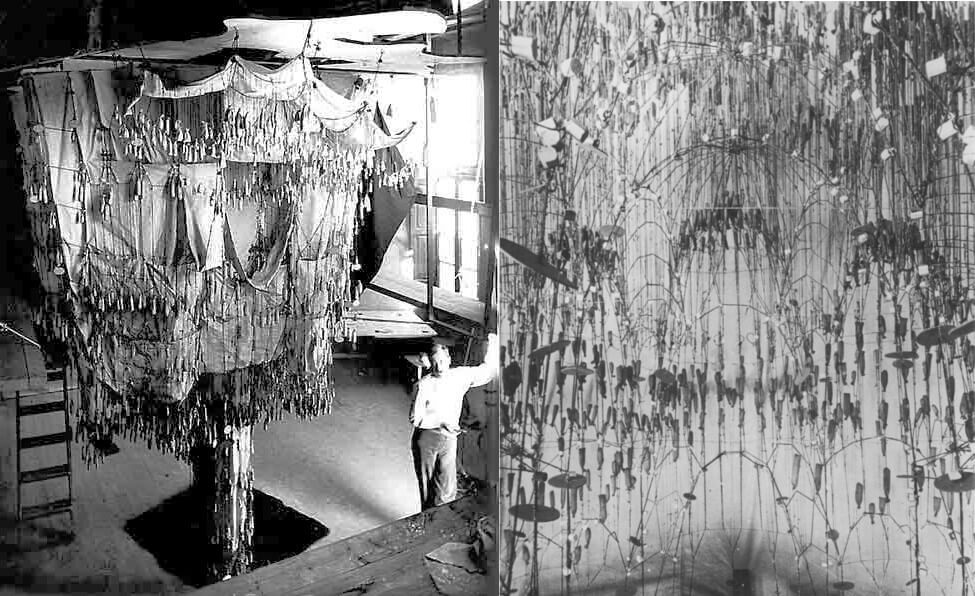
\includegraphics[width=10cm]{Img/GEO/geo-gaudic.jpg}
\centering
\caption{\footnotesize{Maqueta gravitatoria de Gaudí.}}
\label{fig:gaudi}
\end{figure}

Una cadena que cuelga tiene por lo menos cuatro parámetros: su longitud, su peso y los dos puntos a los que está sujetada. Al estar colgando por la acción de la fuerza de gravedad adopta una forma curva, definida por la función explicita de los parámetros de la cadena. A pesar de ser análogo, este es un modelo paramétrico debido a la presencia de parámetros que controlan una forma derivada de una función (calculada por la acción de la gravedad). Así, el diseñador puede modificar  un diseño representado por un modelo visual de forma interactiva y en tiempo real, en este caso mediante arcos catenarios\footnote{Una catenaria es una curva ideal que representa físicamente la curva generada por una cadena, cuerda o cable sin rigidez flexional, suspendida de sus dos extremos y sometida a un campo gravitatorio uniforme.}.

No fue hasta la aparición de las computadoras y el primer programa CAD, \textbf{Sketchpad} \citep{Sutherland:1963:SMG:1461551.1461591} (ver figura \ref{img:sketchpad}) que se facilitó la interacción en tiempo real del diseñador y la computadora \citep{evolved2017}.

\begin{figure}[ht]
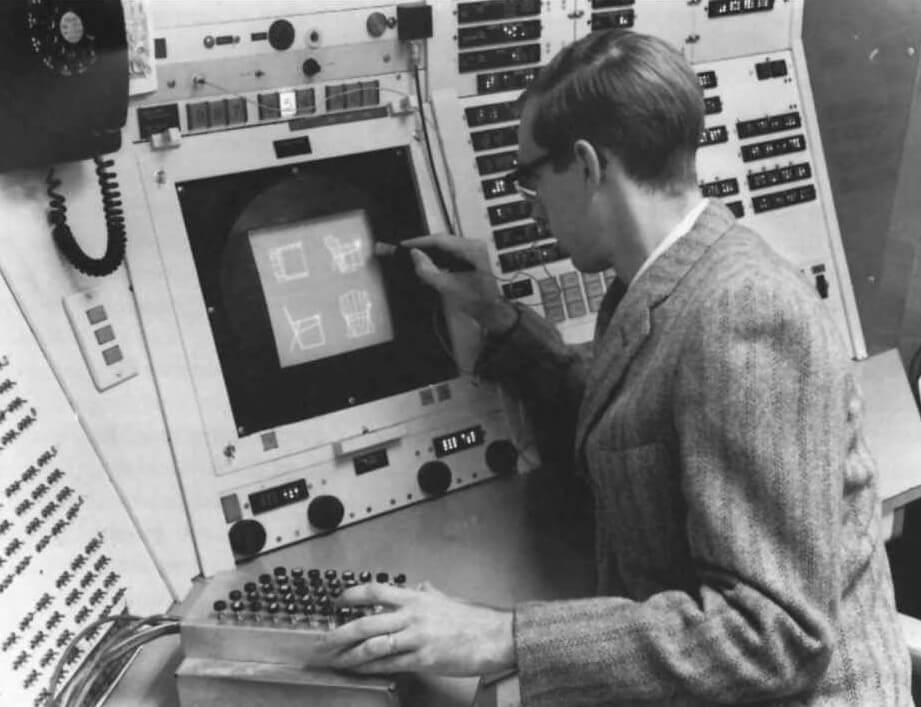
\includegraphics[width=10cm]{Img/GEO/geo-sketchpadc.jpg}
\centering
\caption{\footnotesize{Ivan Sutherland utilizando sketchpad en 1963.
}}
\label{img:sketchpad}
\end{figure}



En este contexto, para comprender el uso de tecnologías CAD es fundamental diferenciar  los conceptos  \textbf{computarización del diseño} y  \textbf{diseño computacional}. El primero indica el uso de la computadora como herramienta de dibujo o representación formal orientado a disciplinas creativas, por ejemplo al realizar arte digital\footnote{El arte digital engloba una serie de disciplinas creativas en las que se utilizan tecnologías digitales en el proceso de producción o en su exhibición.}, mientras que el diseño computacional aborda el diseño con bases en el pensamiento algorítmico, incluyendo el diseño paramétrico y el generativo \citep{Kaled2016}.



\section{Diseño Paramétrico}
\label{cadparam}
El \textbf{Diseño Paramétrico} se entiende en términos generales como un proceso de descripción de una problemática utilizando variables. Actualmente para describir estas variables, los diseñadores introducen valores o algoritmos en un software especializado como \Gls{AutoCAD}\footnote{\url{https://latinoamerica.autodesk.com/products/autocad/overview}}, al modificar las variables se generan una serie de alternativas de soluciones y según el criterio del diseñador, se obtiene la solución final. El diseño paramétrico en su definición contemporánea es únicamente posible creando un modelo paramétrico y se define como un conjunto de ecuaciones que expresan una geometría explícitamente por medio de funciones definidas por parámetros \citep{burry2012new}. En la figura \ref{fig:procesopar} \citep{bohnacker2012generative} se puede analizar el proceso general:

\begin{itemize}
    \item Primero se realiza la abstracción de ideas y los conceptos del diseño. 
    \item A partir de la abstracción se establecen las condiciones geométricas y matemáticas para dar soporte a las ideas iniciales.
    \item Del punto anterior derivan los parámetros y variables necesarios para programar el proceso. 
    \item Finalmente, de la programación se obtiene la representación visual para explorar los resultados. 
\end{itemize}

En todo momento el diseñador puede modificar las condiciones geométricas y matemáticas, los parámetros de la programación y explorar los resultados.

\newline
Mediante el \textbf{diseño iterativo} en inglés \textit{iterative design} \citep{blokdyk2018iterative} se analizan los resultados, se vuelve a trabajar y refinar el modelo diseñado hasta lograr una versión o solución aceptable. 


\begin{figure}[ht]
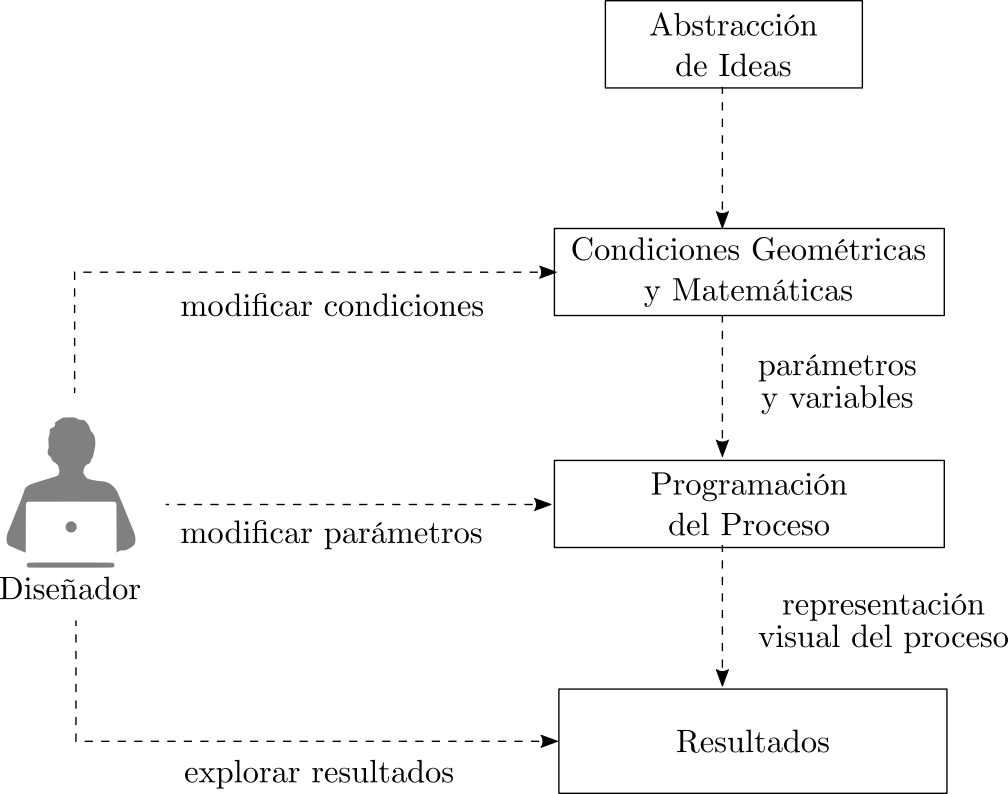
\includegraphics[width=10cm]{Img/CPD/diseno.png}
\centering
\caption{\footnotesize{Proceso general del diseño paramétrico.
}}
\label{fig:procesopar}
\end{figure}

Los modelos paramétricos permiten a los diseñadores alterar y modificar la geometría de manera eficiente sin tener que volver a crear el modelo. De esta manera, la parametrización puede elevar la calidad\footnote{{Capacidad que posee un objeto para satisfacer necesidades.}} y la reutilización de un modelo \citep{Alfaiate2017}. Este enfoque de diseño se lleva a la práctica utilizando  \textbf{paquetes aplicativos} o bien mediante la \textbf{codificación por medio de algoritmos}.

\subsection{Diseño paramétrico mediante paquetes aplicativos}

Los paquetes aplicativos de CAD  son aquellos que se instalan en el ordenador y no requieren del uso de internet, como AutoCAD. En este software, el diseño paramétrico se logra utilizando restricciones aplicadas a la geometría \citep{Autodesk2017} y se clasifican en dos tipos: las \textbf{restricciones geométricas} que controlan las relaciones entre los objetos y las \textbf{restricciones por cota} que controlan los valores de distancia, longitud, ángulo y radio de los objetos. Proporcionan una manera de cumplir con ciertos requisitos que permiten  experimentar con los diseños o hacer modificaciones. Asimismo, las restricciones pueden aumentar su flexibilidad mediante el uso de fórmulas y ecuaciones.\vskip
En el modelo de la figura  \ref{fig:autocad-0} algunas modificaciones en los parámetros pueden hacer cambios automáticamente a otros. Se puede apreciar una restricción mediante la fórmula $d2 = d1*6$ de manera que $d2$ siempre será 6 veces el tamaño de $d1$ (las variables están relacionadas). Por otro lado, el valor del diámetro $dia1$ es independiente a cualquier otro  parámetro \citep{Autodesk2017}. 



\begin{figure}[ht]
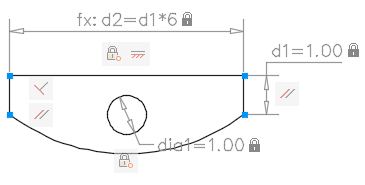
\includegraphics[width=6cm]{Img/CPD/autocad-0.png}
\centering
\caption{\footnotesize{Restricciones en un diseño paramétrico hecho con AutoCAD. }}
\label{fig:autocad-0}
\end{figure}

\subsection{Diseño paramétrico especificado en algoritmos} 
\label{dis:script}
 
Las \textbf{interfaces de secuencias de comandos} en inglés \textit{\gls{scripting}}\footnote{Un script es un programa informático usualmente simple, que por lo general se almacena en un archivo de texto plano. } permiten a los diseñadores/programadores escribir código para automatizar partes del diseño.

El script, con sus parámetros de entrada, funciones explícitas y salidas es una realización arquetípica de la definición matemática de paramétrico \citep{burry2012new}.
Los \textbf{sistemas paramétricos} se basan principalmente en \textbf{principios algorítmicos}, dado que al igual que los algoritmos, toman un valor o un conjunto de valores como entrada, ejecutan una serie de pasos computacionales que transforman la entrada y finalmente producen un valor o un conjunto de valores como salida \citep{Dino2012}. Por lo tanto, las interfaces de scripting disponibles en gran parte de los paquetes CAD están naturalmente predispuestas para generar modelos paramétricos.\vskip
En la figura \ref{fig:script} se muestra un programa para generar una espiral 3D con bloques simples (derecha) mediante expresiones anidadas definidas en código \Gls{AutoLisp} (derecha) \citep{Celani2008}.



\begin{figure}[ht]
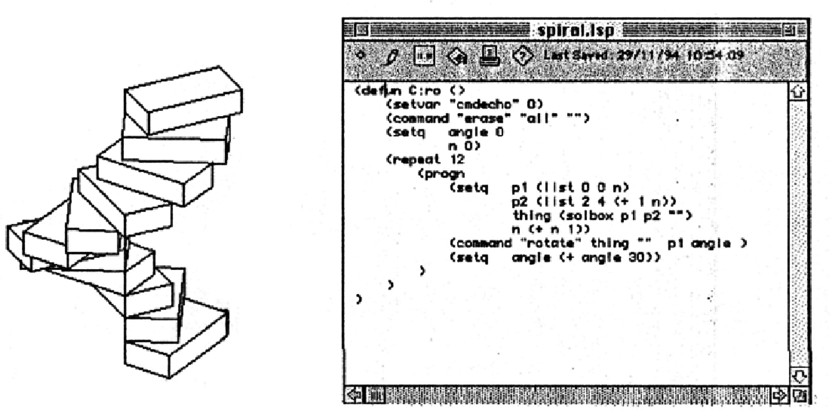
\includegraphics[width=12cm]{Img/CPD/cad-autolisp.jpg}
\centering
\caption{\footnotesize{Programa en código AutoLISP para generar una espiral 3D.}}
\label{fig:script}
\end{figure}

Independientemente de las aplicaciones que se utilicen para el diseño, los modelos resultantes son útiles para realizar estudios que de otra manera serían difíciles, por ejemplo al no contar con el objeto físico. En este aspecto, entra en juego el \textbf{Modelado Geométrico}  \citep{Ramos2011}, haciendo referencia al conjunto de métodos utilizados para definir la forma y otras características de los objetos. Estos métodos son un compendio de las técnicas utilizadas en varias disciplinas, como la Geometría Analítica y Descriptiva, la Topología, la Teoría de Conjuntos, el Análisis Numérico, las Estructuras de Datos, el Cálculo Vectorial y los Métodos Matriciales. Las aplicaciones de estas técnicas abarcan la \textbf{Representación}, \textbf{Visualización} y \textbf{Diseño} de los objetos.




\section{Modelado Sólido}
\label{ref:modelado-solido}
 El \textbf{Modelado Sólido} \citep{Foley-ITC-1990} es una rama del modelado geométrico que  hace hincapié en la aplicabilidad general de los modelos, e insiste en crear solamente modelos ``completos" de los sólidos, es decir, modelos que son adecuados para responder algorítmicamente (sin la ayuda externa del usuario) a cualquier pregunta geométrica que se formule. Se espera que respondan preguntas geométricas típicas que aparecen en las aplicaciones de ingeniería. Por ejemplo:
¿Cuál es el aspecto del objeto?, ¿Cómo puede fabricarse con los procesos de manufacturación disponibles? 
La respuesta podría ser una imagen, un número o una constante booleana. De hecho, incluso podría ser otro modelo sólido \citep{Ramos2011}. 


\vspace{5mm}
Las \textbf{ventajas prácticas del modelado sólido} son:
\begin{itemize}
    \item Agiliza el desarrollo y los detalles del diseño.
    \item Mejora la visualización y la comunicación del diseño.
    \item Elimina los problemas de interferencias del diseño.
    \item Comprueba la funcionalidad y el rendimiento del diseño (sin la necesidad de prototipos físicos).
    \item \textbf{Proporciona de forma automática las características topológicas para la fabricación digital}, necesarias al programar máquinas herramientas de CNC, impresoras 3D, etc.
\end{itemize}


Un sistema de Modelado Sólido maneja dos tipos de información: los \textbf{datos geométricos} y \textbf{los datos topológicos}. Los datos geométricos son aquellos que representan geométricamente los objetos (coordenadas de vértices, ecuaciones de superficies, etc). En cambio, los topológicos se refieren a cómo conectar componentes geométricos para conseguir un modelo \citep{Ramos2011}.

\subsection{Representación geométrica}
\label{repGeo}

Muchos esquemas de representación y particularmente los modelos sólidos utilizan \textbf{poliedros} \citep{cromwell1999polyhedra} con caras, aristas y vértices. Se pueden apreciar en la figura \ref{fig:poli} con 2 ejemplos de poliedros: prisma rectangular (izquierda) y tetraedro (derecha).
A bajo nivel, todos los algoritmos que se utilizan se basan en una única primitiva\footnote{Las formas geométricas se denominan  primitivas por su básica constitución en las partes que la conforman.}: el \textbf{polígono} y los polígonos se dividen en elementos más simples: \textbf{triángulos}.

\begin{figure}[ht]
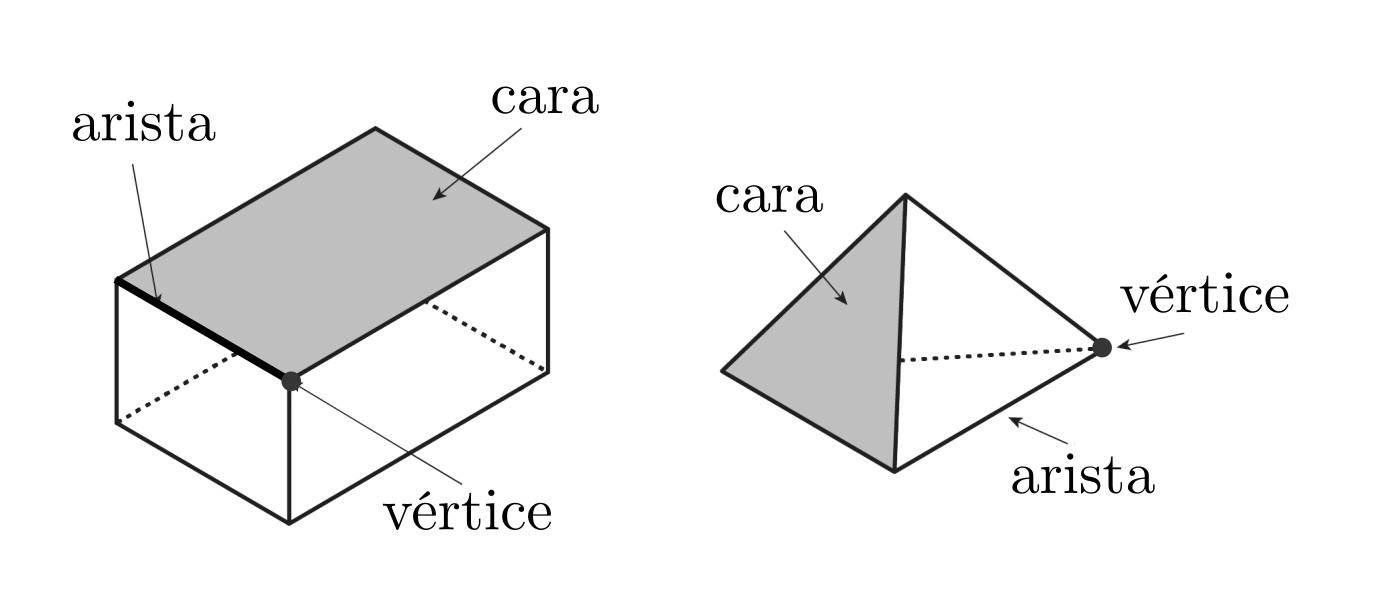
\includegraphics[width=8cm]{Img/GEO/geo-vertex.jpg}
\centering
\caption{\footnotesize{Caras, aristas y vértices en 2 poliedros diferentes.}}
\label{fig:poli}
\end{figure}


\subsubsection{Transformaciones 3D}
En términos matemáticos, es común encontrar la representación de los modelos por medio de \textbf{Matrices} \citep{Gabriela2008} (espacio vectorial 3D), estos deben someterse a ciertas transformaciones antes de que su imagen aparezca en la pantalla de un dispositivo. Las transformaciones geométricas se definen como la relaciones de los puntos entre dos imágenes, son operaciones matriciales sobre los puntos del objeto. Cada  objeto se representa como una matriz constituida por las coordenadas $(x,\ y,\ z)$ de los puntos que lo conforman  \citep{villamarin2015}.

Las transformaciones básicas son:  \textbf{Traslación  3D}, \textbf{Rotación  3D}, \textbf{Escalamiento  3D} y la composición de las mismas para lograr secuencias de transformaciones.
La traslación mueve un objeto con una trayectoria en línea recta de una posición a otra. La rotación mueve un objeto de una posición a otra a lo largo de una trayectoria circular sobre un eje de rotación específico.


\vspace{5mm}
A modo de ejemplo se explica el Escalamiento 3D:

El escalamiento permite cambiar el tamaño de un objeto expandiéndolo o contrayéndolo en sus dimensiones. % \citep{Matias2007}. 
Esto implica el cambio de tamaño de un poliedro, donde cada punto $p = (x,\ y,\ z)$ es transformado por la multiplicación de tres factores de escalamiento: $s_{x}, s_{y}$ y $s_{z}$ a lo largo de los ejes $X,\ Y,\ Z$ respectivamente, de esta forma, las coordenadas del nuevo punto $p^{\prime} = ({x}^{ \prime},\ {y}^{ \prime},\ {z}^{ \prime})$ se obtienen como:
$$
\begin{array}{l@{}l}
{x}^{\prime} = x.s_{x}
\\
{y}^{\prime} = y.s_{y}
\\
{z}^{\prime} = z.s_{z}
\end{array}
$$


Sea $s = (s_{x},\ s_{y},\ s_{z})$ el vector de factores de escalamiento, y $S(s)$ la matriz de
escalamiento, en coordenadas homogéneas \citep{santalo1966geometria} el escalamiento de un punto $p$ en 3D se puede expresar como el producto matricial
$p^{\prime} = p.S(s)$ , es decir (ver ecuación \ref{eq:1}):

\begin{equation}
\begin{array}{rccl}
\left[
\begin{array}{rccl}
{x}^{\prime} & {y}^{\prime} & {z}^{\prime} & 1\\
\end{array}
\right]
\end{array}
=
\begin{array}{rccl}
\left[
\begin{array}{rccl}
x & y & z & 1\newline
\end{array}
\right]
\end{array} 
.
\left[
\begin{array}{rccl}
s_{x} & 0 & 0 & 0\\
0 & s_{y} & 0 & 0\\
0 & 0 & s_{z} & 0\\
0 & 0 & 0 & 1\\
\end{array}
\right]   
\label{eq:1}
\end{equation}
\begin{center}
\footnotesize{Expresión matricial para el escalamiento 3D.}
\end{center}

En la figura \ref{fig:escala} se puede apreciar el escalamiento de un cubo (izquierda) con los factores $s_x=2$, $s_y=2.5$ y $s_z=1.5$. Al aplicar diferentes factores se produce una variación en las proporciones del objeto original dando como resultado el objeto de la derecha \citep{Matias2007}.

\begin{center}
\begin{figure}[ht]
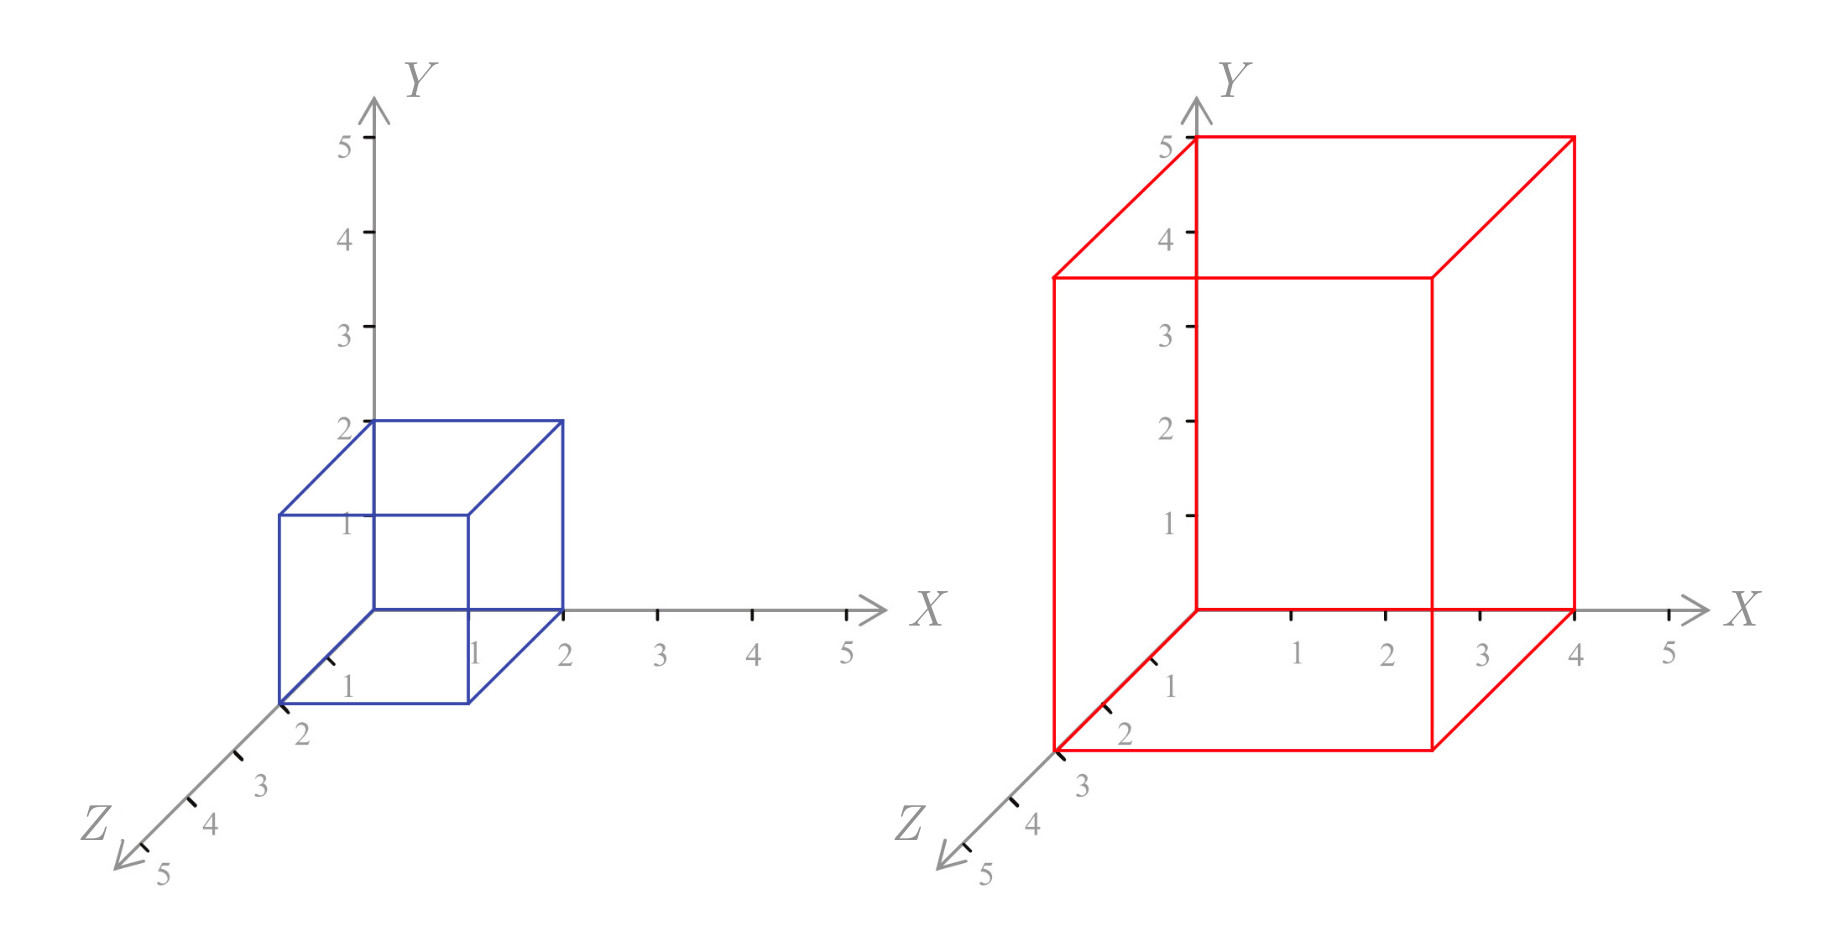
\includegraphics[width=12cm]{Img/GEO/geo-escala0.jpg}
\centering
\caption{\footnotesize{Escalamiento de un cubo.}}
\label{fig:escala}
\end{figure}
\end{center}


El \textbf{visor} o cámara puede ser considerado como un objeto más, respecto a las transformaciones lineales. Sin embargo, el movimiento de los visores tiene sus propias peculiaridades, por lo que conviene estudiar de modo independiente las transformaciones lineales que se aplican a estos objetos. Por ejemplo: El cambio de escala en el visor produce el efecto \gls{zoom} (acercar/alejar) \citep{Ramos2011}.

\subsubsection{Topología de los modelos sólidos}
\newline
Conocer las características topológicas de los poliedros es importante para la construcción de los modelos sólidos y especialmente para su validación. 

Los sólidos están definidos en el espacio Euclídeo $E^3$, ocupando una determinada porción de ese espacio. Por lo tanto, se considera un sólido como un conjunto de $E^3$. Obviamente no todos los subconjuntos del espacio Euclídeo son sólidos (por ejemplo un punto aislado no es un sólido). Para que un sólido abstracto resulte útil como elemento de representación debe poseer las siguientes propiedades: \citep{Torres2014}:

\begin{itemize}
    \item \textbf{Clausura}. 
    Toda operación efectuada entre un sólido o entre diversos solidos debe producir otro sólido.
    \item \textbf{Finitud}. 
    Ocupa una porción finita del espacio en el que el encuentra inmerso.
    \item \textbf{Frontera determinista}. 
    Debe definir de forma no ambigua la región del espacio que se corresponde con su interior y la que corresponde con su exterior.
    
    \item \textbf{Rigidez}. Los sólidos no se modifican al trasladarlos o rotarlos. O lo que es lo mismo, dos sólidos que se diferencian tan solo en una transformación son el mismo sólido.
    \item \textbf{Homogeneidad tridimensional}. Todas las partes del sólido deben tener la misma dimensionalidad, debe ser tridimensional $E^3$ en todos sus puntos. En la figura \ref{fig:geo-noregular} se ilustra un objeto que no posee homogeneidad tridimensional (no sólido), contiene elementos 2D (cara que cuelga) y 1D (arista que cuelga)  \citep{Torres2014}.
\end{itemize}



\begin{figure}[ht]
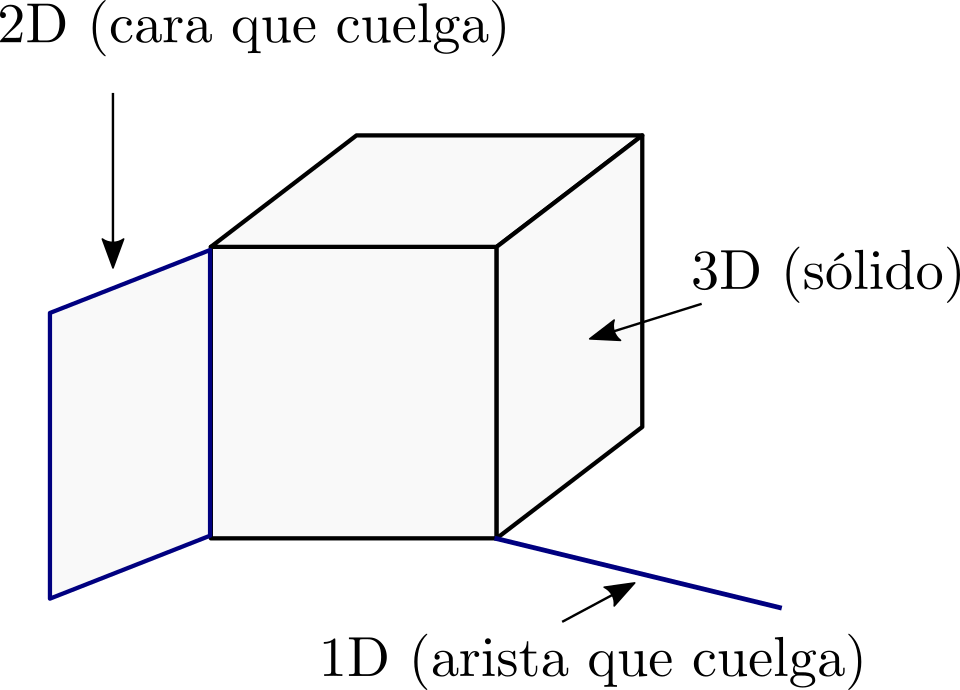
\includegraphics[width=6cm]{Img/GEO/geo-noregular.png}
\centering
\caption{\footnotesize{Objeto sin homogeneidad tridimensional.} }
\label{fig:geo-noregular}
\end{figure}


A continuación se estudia la topología de algunos poliedros que satisfacen las condiciones para el modelado sólido: Los poliedros simples, no simples y los objetos de Euler.\newline

\subsubsection{Poliedros simples y no simples}\newline
    Un \textbf{poliedro simple} es aquél que puede ser transformado de forma continua en una esfera, o sea, es topológicamente equivalente a una esfera.

    La \textbf{Fórmula de Euler} para los poliedros simples
    establece que \textquote{\textit{para un poliedro simple se cumple que el número de vértices $V$, menos el número de aristas $A$, más el número de caras $C$}} \cite{Ramos2011} es igual a 2, es decir (ver \ref{eq:2}):

    \begin{equation}
    V - A  +  C = 2
    \label{eq:2}
    \end{equation}
    
    Los poliedros regulares forman un subconjunto de los poliedros simples, cuya característica principal es que todas sus caras (polígonos) son iguales, según la fórmula anterior se puede demostrar que sólo existen 5 poliedros regulares: tetraedro, hexaedro o cubo, octaedro, dodecaedro e icosaedro.
    
    
Los \textbf{poliedros no simples} son los equivalentes topológicos de cualquier objeto sólido con huecos, por lo que son muy útiles en el Modelado Sólido \citep{Ramos2011}. 

    
    Para clasificar los poliedros se recurre al concepto de \textbf{número de conectividad}  $(n)$. Si la superficie de un poliedro se puede dividir en dos regiones separadas mediante un camino cerrado trazado a lo largo de sus aristas, se dice que tiene conectividad $n = 0$. La esfera es un cuerpo que siempre cumple con esa condición, por ende, cualquier poliedro de conectividad $0$ (simple) puede ser transformado en una esfera. Este fenómeno se aprecia con el poliedro simple regular (icosaedro) ilustrado a la izquierda de la figura \ref{fig:polino}. 
    Por otro lado, el objeto de la derecha cuenta con caminos cerrados que no dividen a su superficie en dos partes separadas (contiene un hueco). A estos poliedros se les asigna un número de conectividad mayor que $0$ y por ende, al contener huecos se los denomina \textbf{no simples}.
    
    
    \begin{figure}[ht]
    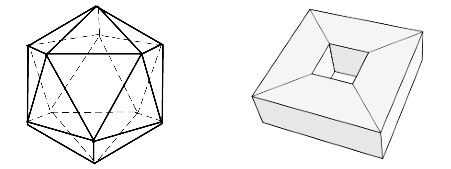
\includegraphics[width=8cm]{Img/GEO/geo-simple-nosimple.png}
    \centering
    \caption{\footnotesize{Poliedro simple y poliedro no simple.}}
    \label{fig:polino}
    \end{figure}
    
    Si bien los poliedros simples y no simples son sólidos, la fórmula de Euler establece condiciones necesarias, pero no suficientes para que un objeto sea un poliedro. Se pueden construir objetos que satisfagan la fórmula, pero que no acoten un volumen, sin más que añadir una o más caras o aristas colgantes. \textbf{Se requieren de otras restricciones para garantizar que un objeto sea un sólido}.

\subsubsection{ Objetos de Euler }
A $g$ se conoce como \textbf{orden o grado del objeto} y también como \textbf{orden de la superficie}. Así, una esfera equivale a $g = 0 $, un toro, topológicamente hablando, puede considerarse como una esfera con 1 asa ($g = 1$) y así sucesivamente según la cantidad de huecos que tenga el objeto. En la figura \ref{fig:asas} se muestran 3 objetos diferentes representados  como \textbf{esferas con asas} ($g = 0$, $g = 1$ y $g = 2$) respectivamente  \citep{Annenberg}.
 
   \begin{figure}[ht]
    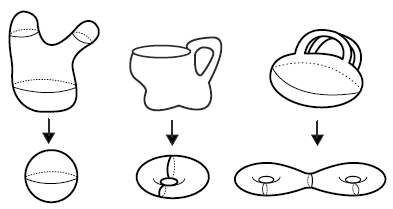
\includegraphics[width=10cm]{Img/GEO/geo-asas.png}
    \centering
    \caption{\footnotesize{Objetos diferentes que se representan como esferas con $g$ asas.}}
    \label{fig:asas}
    \end{figure}
 
 Los objetos cerrados tridimensionales de orden $g \geq 0 $ que verifican ciertos requisitos de construcción se denominan \textbf{objetos de Euler}. Estos requisitos son:
\begin{itemize}
\item Todas sus caras (curvas o planas) han de ser discos topológicos\footnote{Una región, plana o no, que pueda ser transformada en un cuadrado se llama disco topológico.}, es decir que no tienen huecos ni puntos aislados en ellas. 
\item Cada arista une sólo dos caras y todas finalizan en un vértice en
cada extremo.
\item Como mínimo tres aristas se unen en un vértice. 
\end{itemize}

En todos los objetos de Euler se cumple que (ver ecuación \ref{eq:3}):


\begin{equation}
V - A + C  = 2(S-P)
\label{eq:3}
\end{equation}

\begin{description}
%\item $A$: Aristas
%\item $C$: Caras
%\item $V$: Vértices
\item $S$: número de superficies inconexas del objeto.
\item $P$: total de pasajes (túneles) en el objeto.
\end{description}

Como el número de pasajes en un objeto es igual al total de ``asas” o agujeros que posea, ocurre que en la ecuación anterior $P$ es igual al orden del objeto $(P = g)$.\vskip
El significado de $S$ se puede visualizar en la figura \ref{fig:euler} que muestra tres objetos eulerianos, con una, dos y tres superficies inconexas. $S = 1$, $S = 2$ y $S = 3$ respectivamente \citep{Ramos2011}.

\begin{figure}[ht]
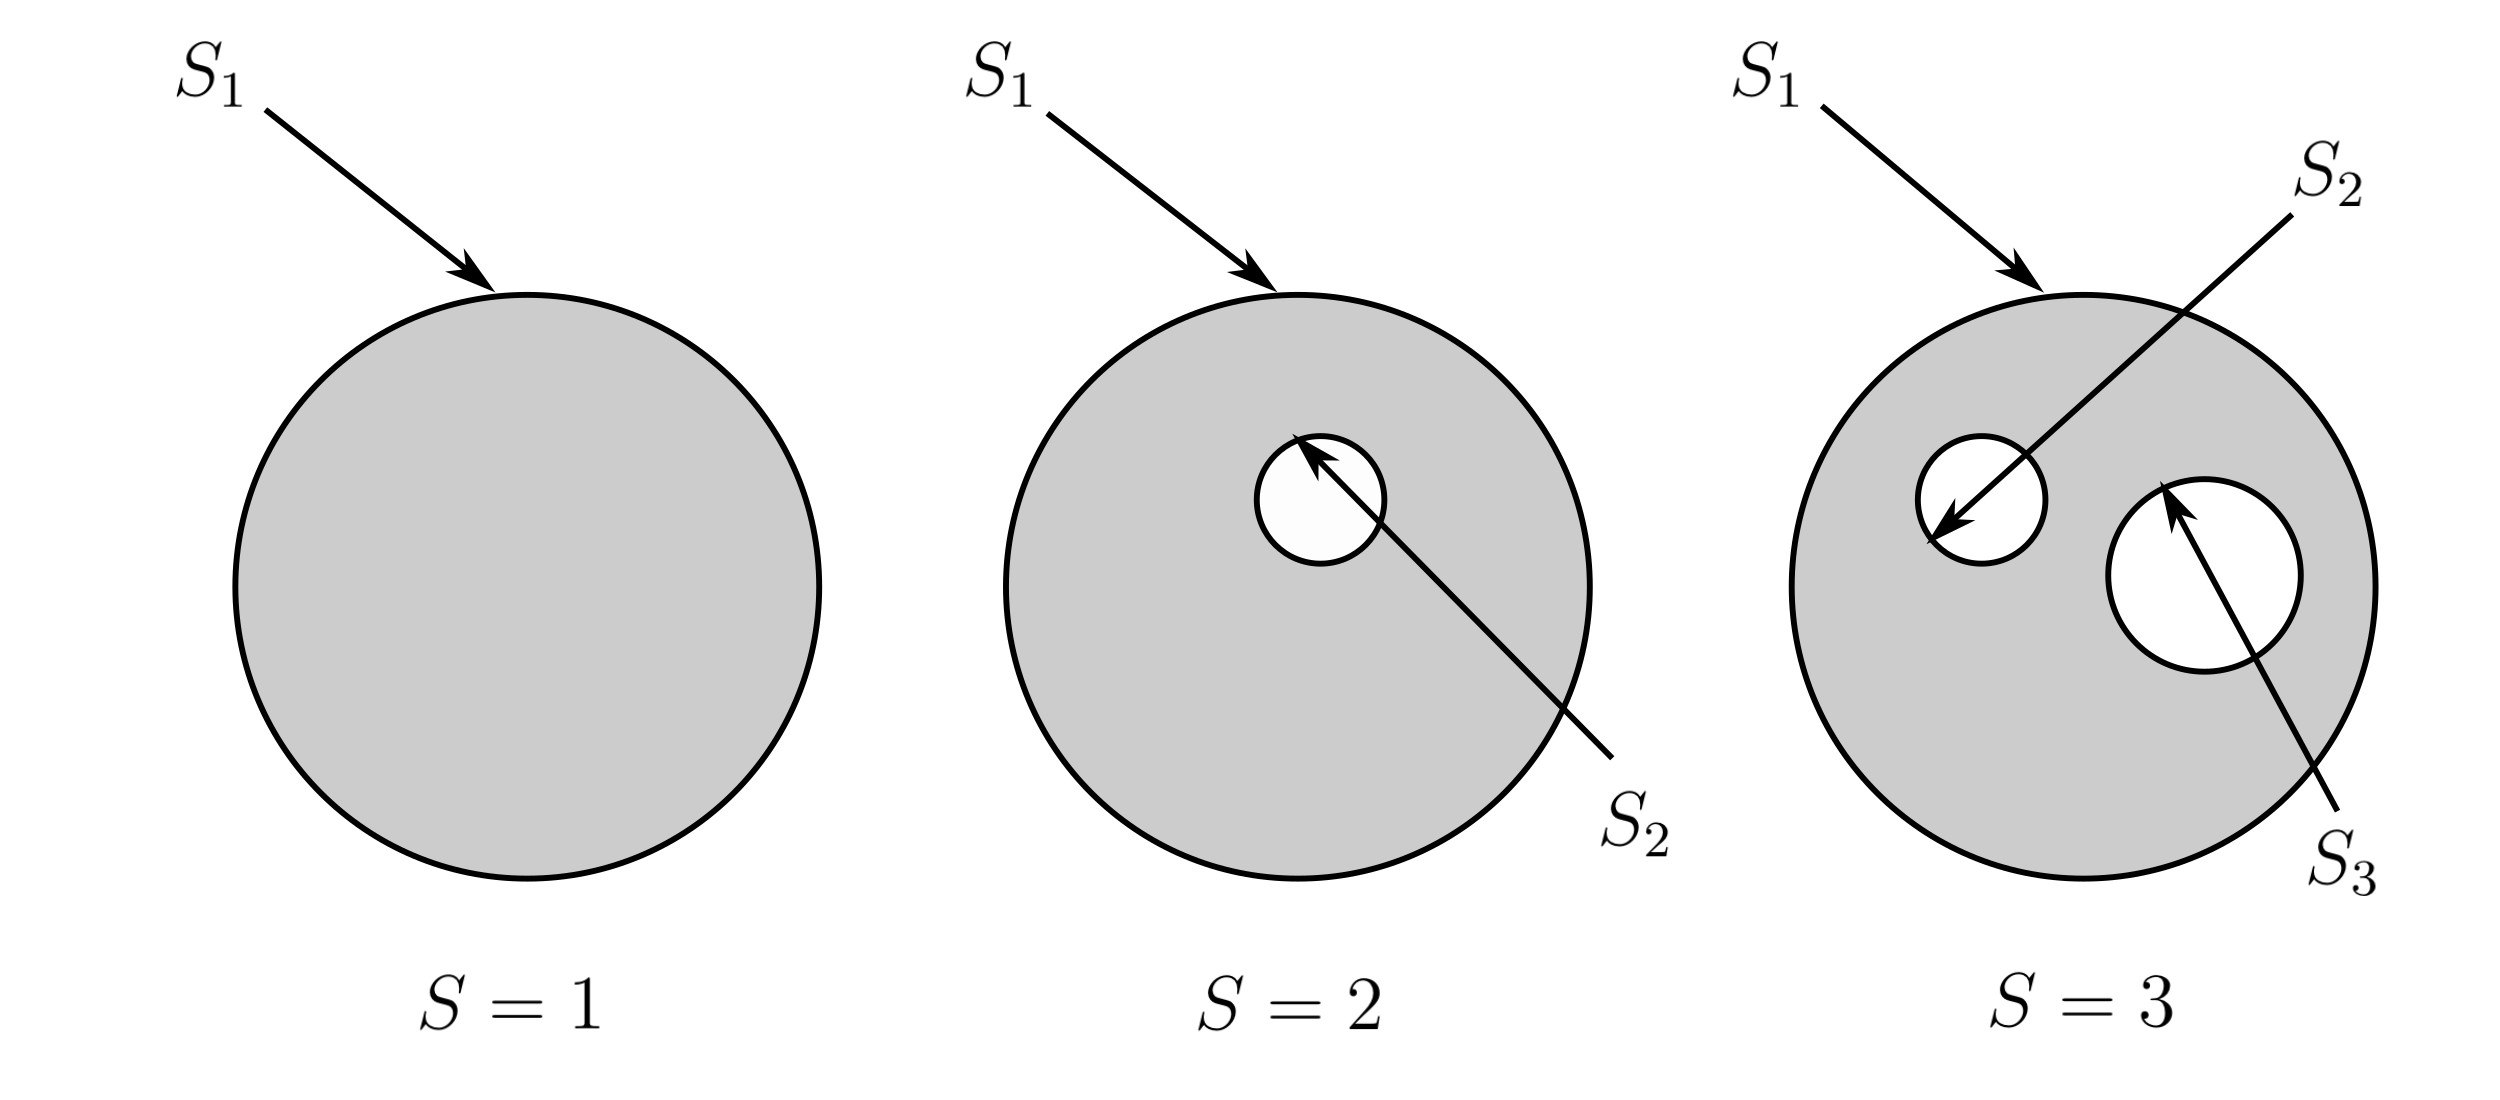
\includegraphics[width=11cm]{Img/GEO/geo-euler0.jpg}
\centering
\caption{\footnotesize{Objetos de Euler con diferentes valores de $S$ (número de superficies inconexas)}}
\label{fig:euler}
\end{figure}

La figura \ref{fig:euler1} ilustra tres objetos eulerianos, si bien estos cuentan con diferentes número de vértices $V$, aristas $A$ y caras $C$, cuando $S = 1$ y $P = 0$ (no poseen huecos) la \ref{eq:3} se reduce a la ecuación de Euler para poliedros simples \ref{eq:2}. Se verifica que en los tres casos se cumple la igualdad, por ende, estos objetos se representan como poliedros simples \citep{Ramos2011}.


\begin{figure}[ht]
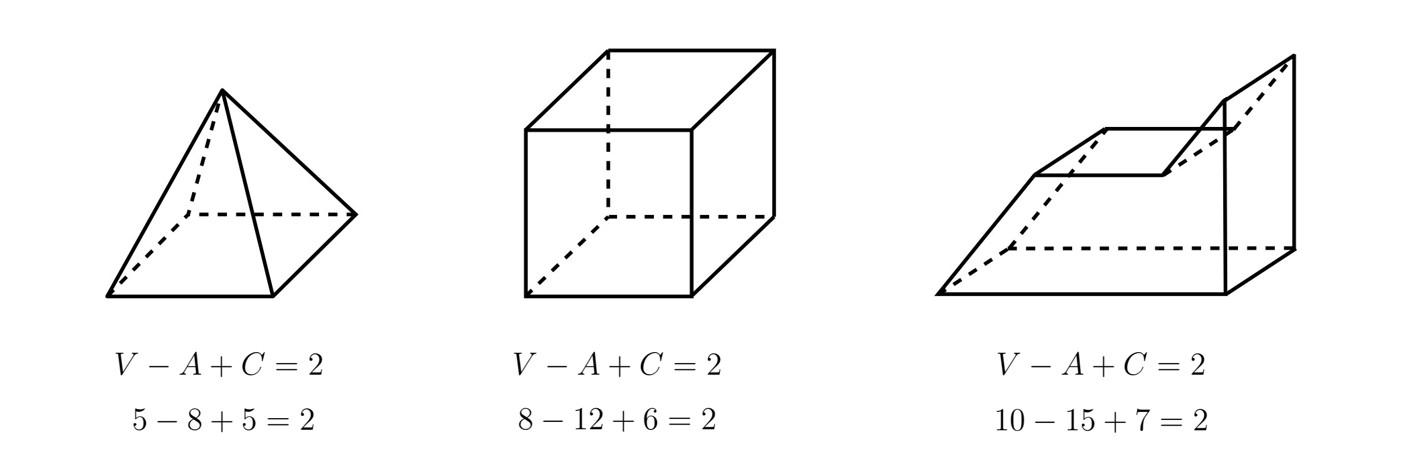
\includegraphics[width=14cm]{Img/GEO/geo-euler1.jpg}
\centering
\caption{\footnotesize{Ejemplos de objetos de Euler con diferentes números de vértices $V$, aristas $A$ y caras $C$.}}
\label{fig:euler1}
\end{figure}


En la figura \ref{fig:euler2} se muestran dos objetos con diferentes $P$. 
El objeto de la izquierda, aunque posee una cavidad, esta no llega a atravesar el modelo $P=0$. Se trata de un objeto sólido topológicamente equivalente a una esfera, es decir, de grado $g = 0$.\newline
Por otro lado, el objeto de la derecha (ver figura \ref{fig:euler2}) es de grado $g = 1$ (posee un túnel que lo atraviesa) $P=1$. Es un sólido topológicamente equivalente a un toro \cite{Ramos2011}.\newline


\begin{figure}[ht]
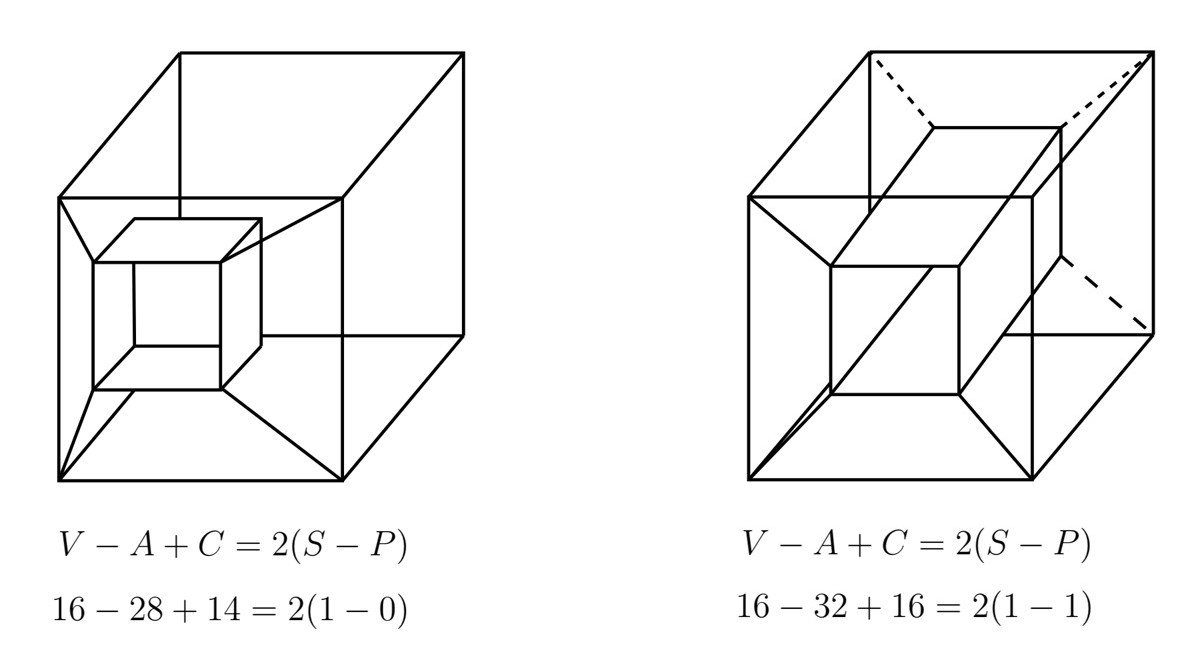
\includegraphics[width=10cm]{Img/GEO/geo-euler2.jpg}
\centering
\caption{\footnotesize{Objetos eulerianos de $g= 0$ y $g=1$, respectivamente. }}
\label{fig:euler2}
\end{figure}


\subsubsection{Representación por atlas}
Uno de los puntos clave en el modelado con poliedros es cómo se registra su información topológica, es decir, las relaciones entre los vértices, aristas y caras que los definen.
La forma más simple y directa para representar los poliedros consiste en describir cada cara por separado, señalando explícitamente cómo han de unirse. Este método de representación se conoce como \textbf{atlas}. 
La figura \ref{fig:atlascubo} muestra el atlas de un cubo, el valor del centro indica el número de cara y los números cercanos al borde indican el número de arista correspondiente a cada cara 
\citep{Ramos2011}.

\begin{figure}[h]
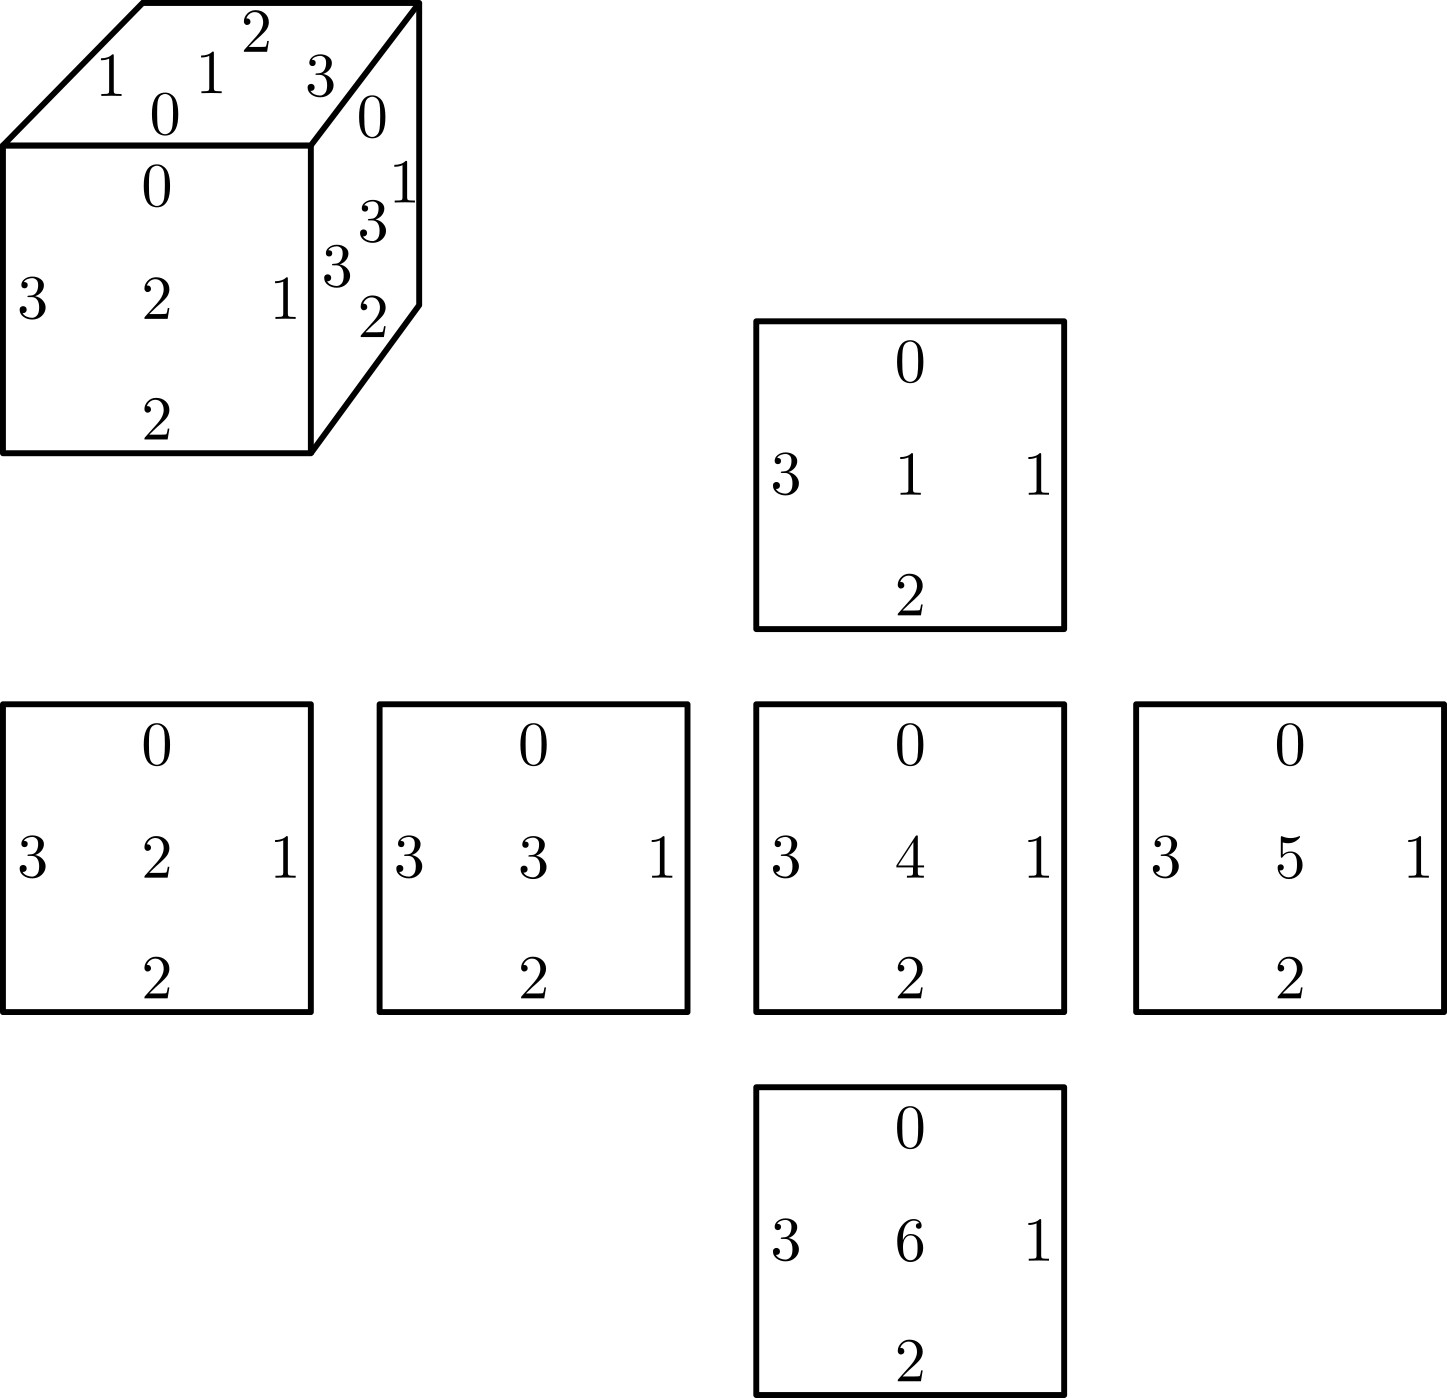
\includegraphics[width=7cm]{Img/GEO/geo-atlas0.jpg}
\centering
\caption{\footnotesize{Atlas de un cubo. }}
\label{fig:atlascubo}
\end{figure}

Cada eje se etiqueta con un par de números indicando la cara y el número de la arista de la cara. Así el par $(1,\ 0)$ se interpreta como la arista $0$ de la cara $1$. Cada unión de dos aristas se especifica por dos pares de números, identificando las aristas que se unen. De esta forma, el atlas se puede representar como una matriz (ver \ref{eq:atlas}):


\begin{equation}
\begin{array}{c@{}c@{}c@{}c}
 \begin{array}{cc}
         [(1,0) & (2,0)]
  \end{array} & \begin{array}{cc}
         [(1,1) & (5,0)]
  \end{array} & \begin{array}{cc}
         [(1,2) & (4,0)]
  \end{array} &
  \begin{array}{cc}
         [(1,3) & (3,0)] 
  \end{array}
  \\
  \begin{array}{cc}
         [(2,1) & (3,3)]
  \end{array} & \begin{array}{cc}
         [(2,3) & (6,2)]
  \end{array} & \begin{array}{cc}
         [(2,3) & (5,1)] 
  \end{array} &
  \begin{array}{cc}
         [(3,1) & (4,3)]
  \end{array}
  \\
  \begin{array}{cc}
         [(3,2) & (6,3)]
  \end{array} & \begin{array}{cc}
         [(4,1) & (5,3)]
  \end{array} & \begin{array}{cc}
         [(4,2) & (6,0)] 
  \end{array} &
  \begin{array}{cc}
         [(5,2) & (6,1)] 
  \end{array}

\end{array}
\label{eq:atlas}
\end{equation}  

\begin{center}
\footnotesize{Representación matricial del atlas}
\end{center}

Además de especificar qué aristas están unidas, se debe decir cómo unirlas. La figura \ref{fig:atlas0} muestra dos formas diferentes de unir un par de aristas. La primera, mostrada a la izquierda, es la unión con \textbf{orientación conservadora}, se obtiene como resultado un cilindro. La segunda (derecha) tiene \textbf{orientación inversora}, se obtiene una cinta de moebius \citep{Ramos2011}. Para unir esas dos aristas hay que hacer coincidir los números de cada una de ellas. Si se hace mediante la orientación conservadora se obtiene un cilindro y con la orientación inversora una \textbf{cinta de Moebius}\footnote{La cinta de Möbius o Moebius es una superficie con una sola cara y un solo borde. Tiene la propiedad matemática de ser un objeto no orientable.}.

\begin{figure}[h]
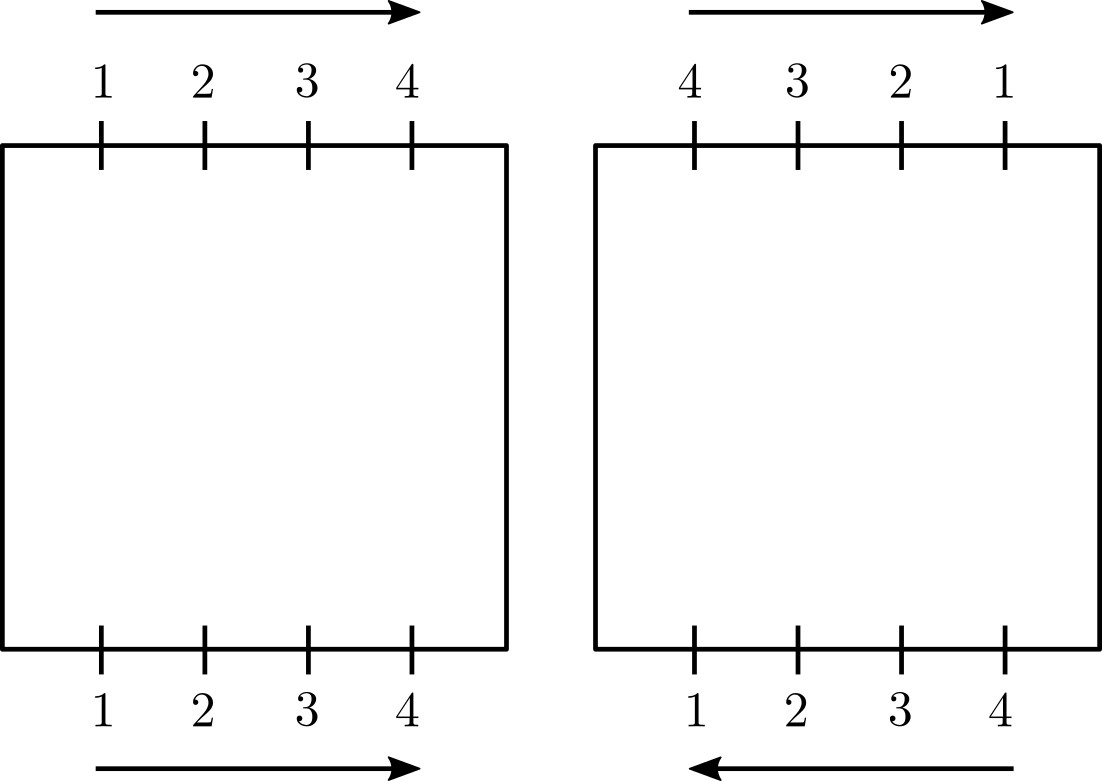
\includegraphics[width=6cm]{Img/GEO/geo-atlas1.jpg}
\centering
\caption{\footnotesize{Orientación conservadora y Orientación inversora.}}
\label{fig:atlas0}
\end{figure}

Para especificar en el atlas de qué forma se van a unir las aristas, se utiliza la \textbf{paridad de transición} que es número $\pm 1$ (+ 1 si es conservadora, -1 si es inversora), unido al par de aristas. La figura \ref{fig:atlas1} presenta tres ejemplos de esta notación: Paridad de transición de una esfera (izquierda), de un toro (centro) y a la derecha de una Botella de Klein (se puede observar la paridad de transición $-1$) \citep{Ramos2011}.

\begin{figure}[h]
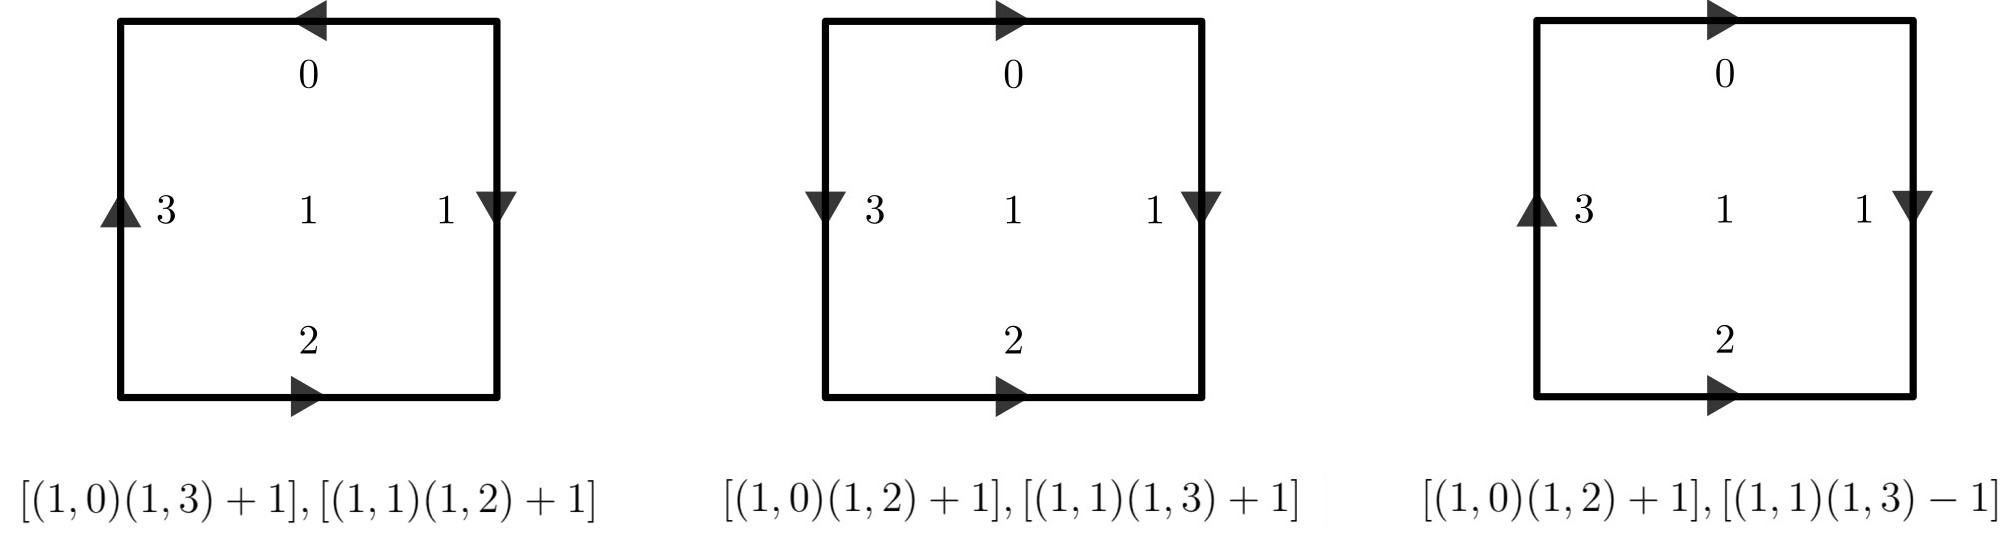
\includegraphics[width=15cm]{Img/GEO/atlas3.jpg}
\centering
\caption{\footnotesize{Paridad de transición de una Esfera, un Toro y una Botella de Klein.}}
\label{fig:atlas1}
\end{figure}

\vspace{5mm}
Si se utilizan uniones no conservadoras en un atlas se consiguen algunas curiosidades matemáticas llamadas \textbf{superficies no orientables}, como la \textbf{cinta de Moebius} y la \textbf{botella de Klein}\footnote{En topología, una botella de Klein es una superficie no orientable abierta cuya característica de Euler es igual a $0$; no tiene interior ni exterior.} (ver figura \ref{fig:atlas2}). La cinta de Moebius posee una curiosa particularidad. Si se recorre la cinta comenzando en un punto cualquiera, y se da una vuelta completa, como se trata de una cinta bidimensional, cuando se llegue al punto de partida se observará que la derecha e izquierda están intercambiadas. 
Si se parte de una cinta de Moebius y se cierra aplicando una orientación conservadora, se obtiene una botella de Klein (no orientable), que no se puede construir en un espacio tridimensional sin que se auto interseque.
Este tipo de superficies se llaman \textbf{no orientables} y se producen al efectuar uniones no conservadoras entre sus aristas. Por el contrario, si en la superficie nunca se intercambian la izquierda y derecha, entonces se dice que la superficie es \textbf{orientable} \citep{Ramos2011}.

\begin{figure}[h]
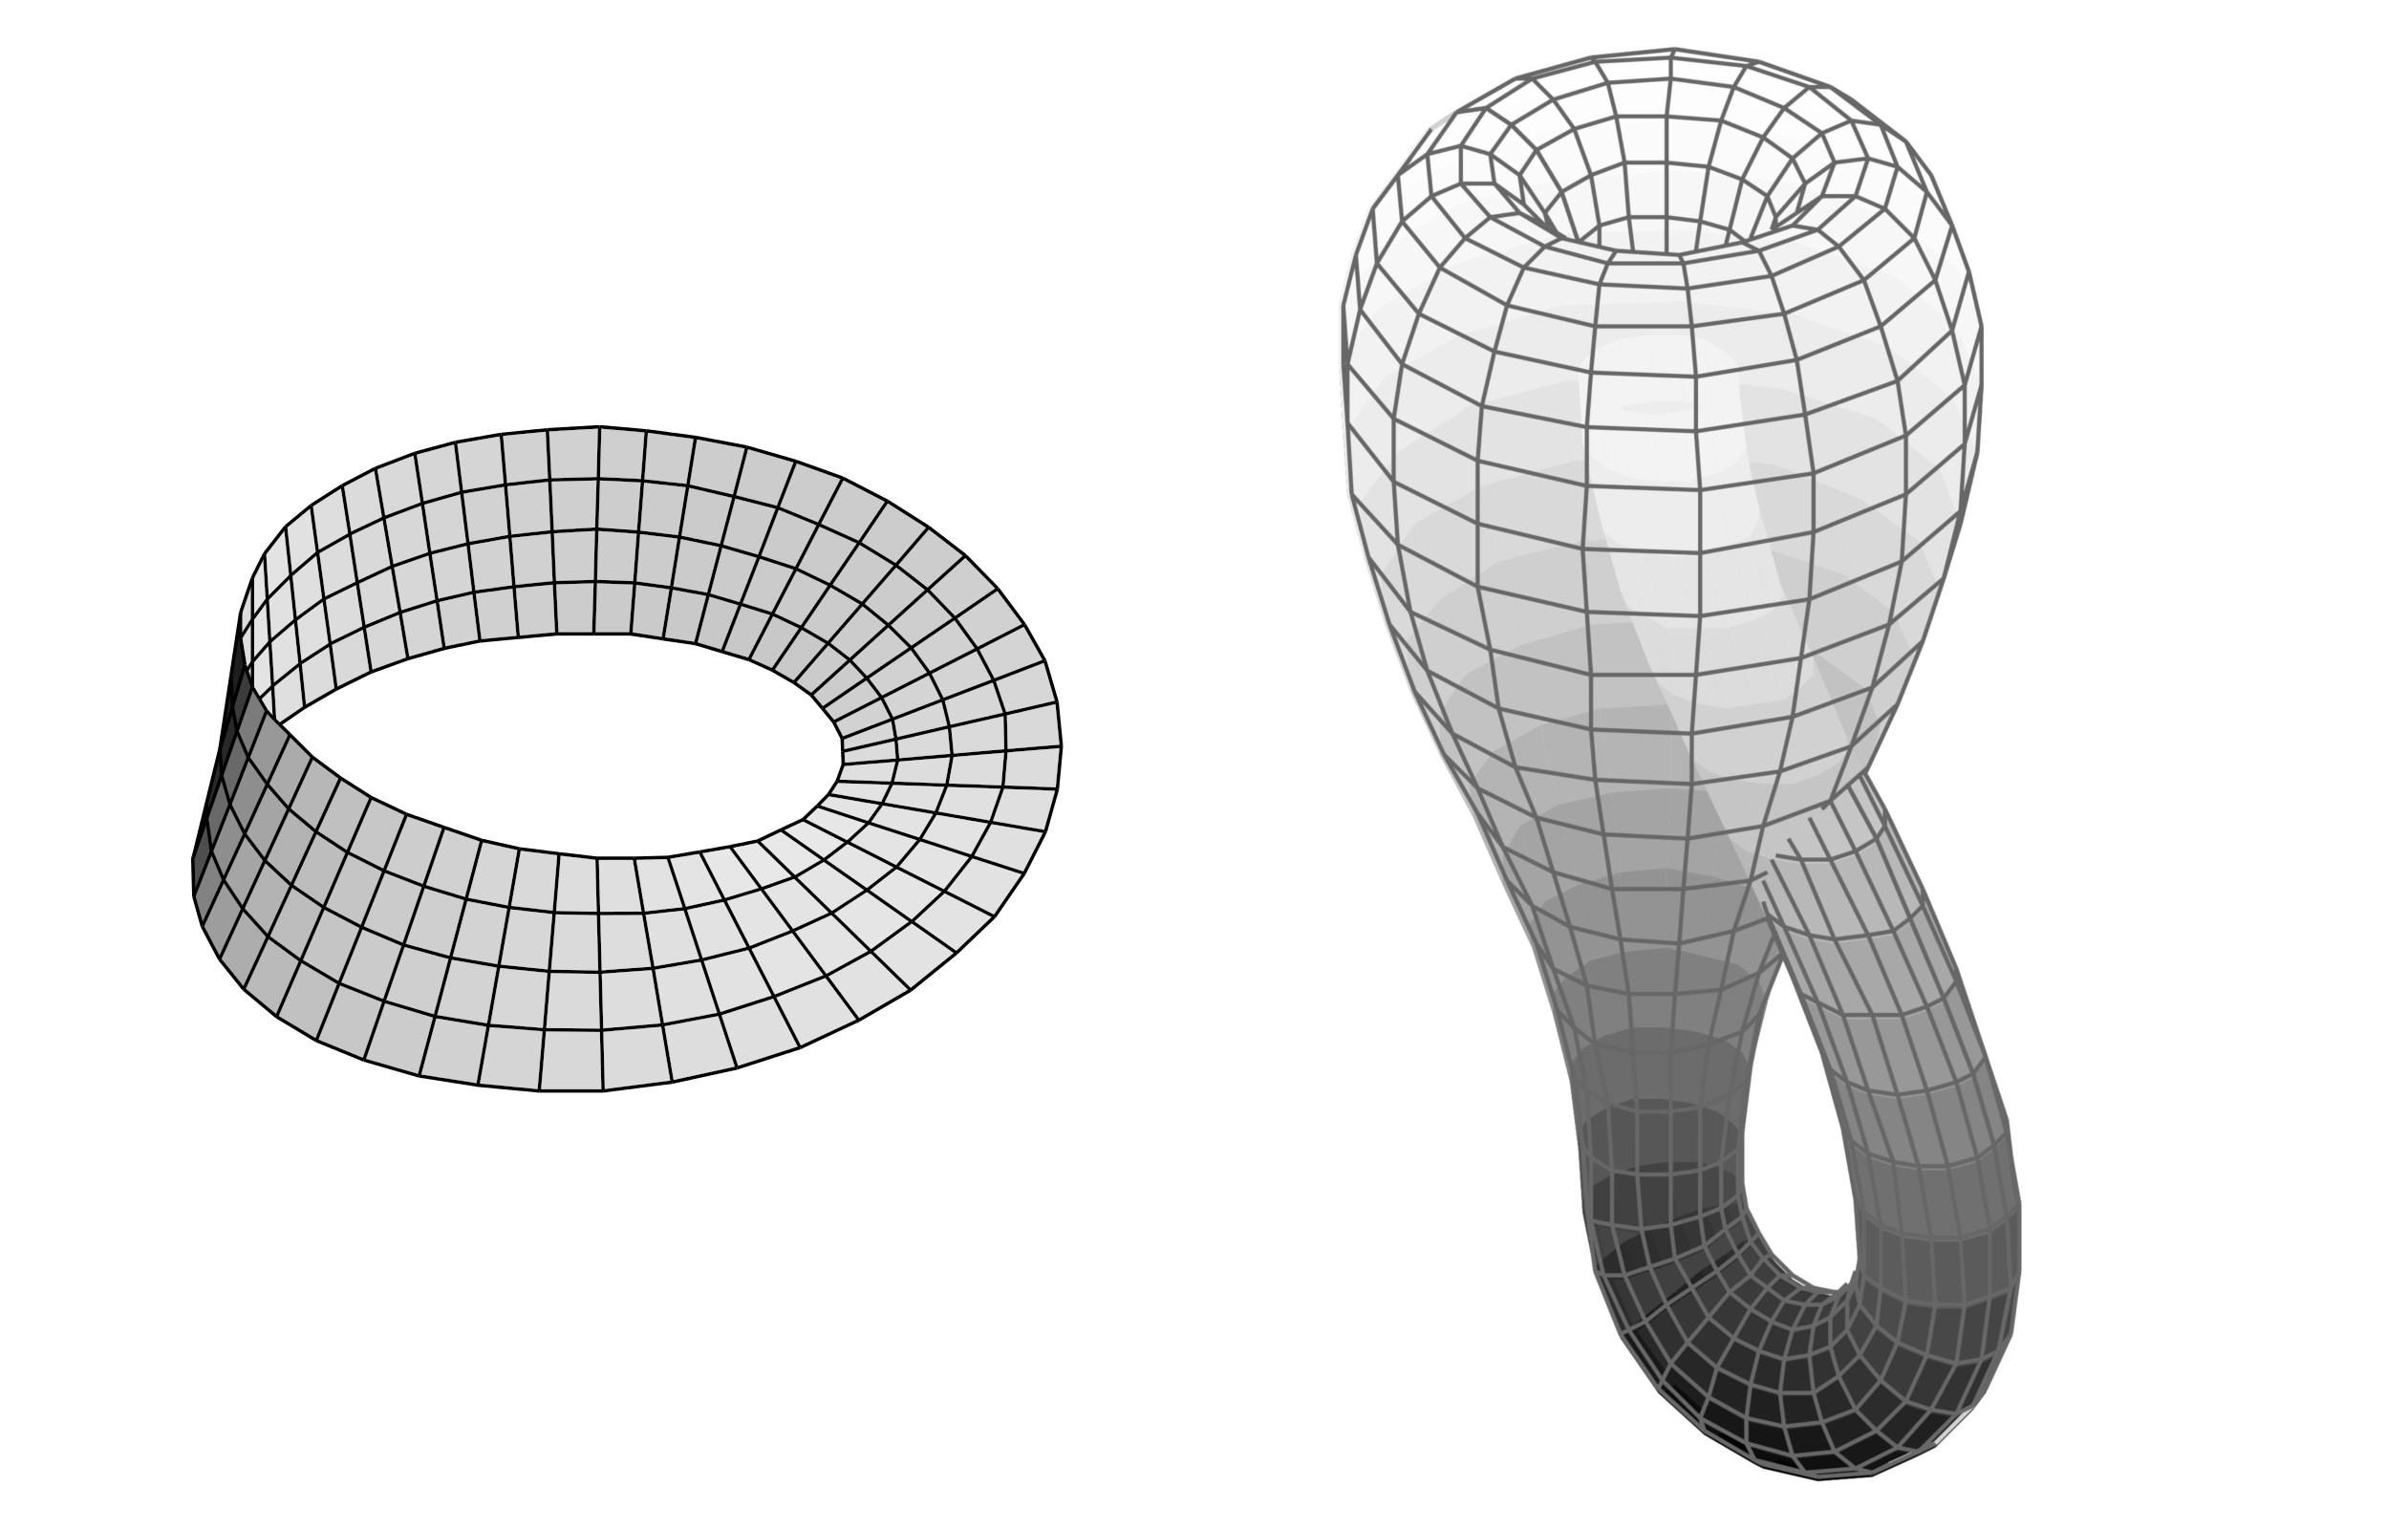
\includegraphics[width=10cm]{Img/GEO/geo-mobius.jpg}
\centering
\caption{\footnotesize{Superficies no orientables. Cinta de Moebius y Botella de Klein.}}
\label{fig:atlas2}
\end{figure}

\textquote{\textit{%Habíamos visto que 
Para que cualquier superficie cerrada tridimensional sea consistente, debe ser topológicamente equivalente a una esfera con ``$g$'' asas. Ahora se añade otra condición más: \textbf{debe ser orientable}}} \citep{Ramos2011}.\newline



\subsubsection{Representación mediante operadores Booleanos. }

Para construir objetos sólidos complejos se pueden utilizar operaciones entre conjuntos, tales como unión $(\cup)$, intersección $(\cap)$ y diferencia ($-$). A estos operadores se les conoce en modelado como \textbf{Operadores Booleanos} \citep{Ramos2011}. Al aplicarlos sobre objetos simples se pueden construir modelos más complejos. Es fundamental que los modelos obtenidos sean íntegros (topológicamente válidos), y que además sean \textbf{dimensionalmente homogéneos}, es decir, que su dimensión sea igual a la de los objetos que se combinan. En la figura \ref{fig:booleano1} se pueden apreciar los resultados de las operaciones booleanas entre los objetos A(esfera) y  B(cubo). $A \cup B$,  $A \cap B$, $A - B$  y  $B - A$  respectivamente \citep{Zhou2018}.

\begin{figure}[ht]
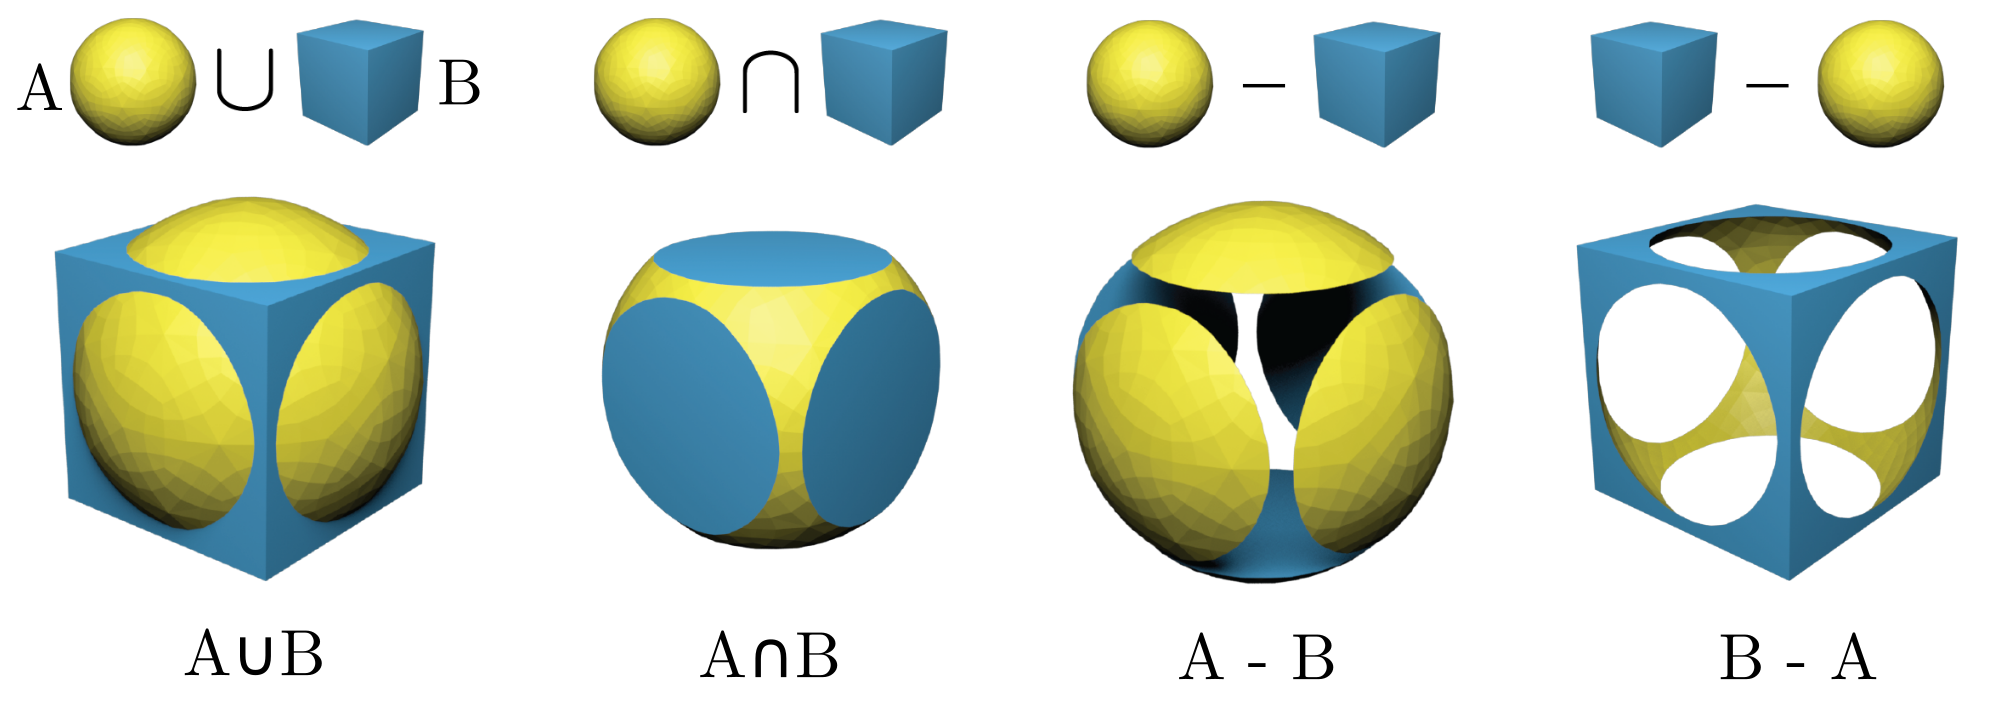
\includegraphics[width=10cm]{Img/GEO/boolean55.png}
\centering
\caption{\footnotesize{Operaciones booleanas entre una esfera y un cubo.}}
\label{fig:booleano1}
\end{figure}

\vspace{5mm}

La aplicación de una operación booleana ordinaria a objetos sólidos no necesariamente produce otro objeto sólido. 
Para evitar esta situación se utiliza el conjunto de \textbf{operadores regularizados} \citep{Ramos2011}, que preservan la homogeneidad dimensional. Se representan por $\cup^*$, $\cap^*$ y $-^*$ y se definen de manera que las operaciones con sólidos siempre generen sólidos.
En la figura \ref{solucion-solido} se muestra un ejemplo donde la intersección $A (\cap) B$ entre dos objetos válidos 3D obtiene como resultado un objeto con una cara que cuelga 2D (no sólido). La solución es efectuar una serie de operaciones matemáticas $i(A (\cap) B)$ de manera que se eliminen los componentes 2D, 1D. Entonces, la intersección ordinaria se reemplaza por la intersección regularizada ($ A \cap^* B$) \citep{Torres2014} asegurando que siempre se generen objetos sólidos.
 

\begin{figure}[ht]
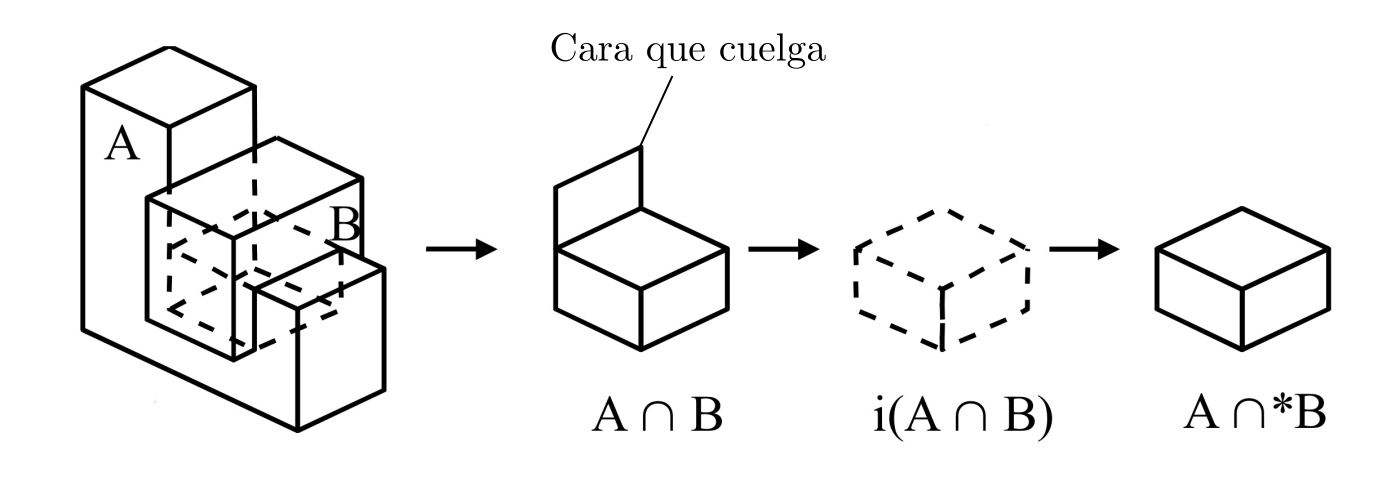
\includegraphics[width=11cm]{Img/GEO/geo-booleano2.png}
\centering
\caption{\footnotesize{Intersección no regularizada ($\cap$) y regularizada ($\cap^*$) de dos sólidos.}}
\label{solucion-solido}
\end{figure}


\subsection{Visualización}
\label{visGeo}

Un elemento indispensable para visualizar modelos 3D en una pantalla es la \textbf{Síntesis de imágenes}, definida como el  \textquote{\textit{campo de la informática gráfica que se dedica principalmente al estudio y desarrollo de procesos para sintetizar imágenes raster}} \cite{Ramos2011}. 
Las computadoras deben realizar un conjunto de operaciones elementales  para conseguir pasar de la \textbf{representación de un modelo geométrico} tridimensional a su imagen plana en pantalla (2D), pero que para la impresión del observador parezca estar contemplando un sistema de visualización en el mundo real en 3D. \vskip
Esquemáticamente, el objetivo principal de un sistema gráfico\footnote{Sistema gráfico se refiere al conjunto de programas y herramientas auxiliares que permiten la síntesis de imágenes raster, a partir de un modelo vectorial 3D.} se resume en la figura \ref{fig:grafica3}: la visualización o \textbf{rendering} se produce en función de las condiciones establecidas por el observador, cámara o visor $f(visor)$ \citep{Ramos2011}. 
Es necesario el visor para generar una imagen bidimensional discreta (raster) a partir de un espacio vectorial 3D, lo que implica no poder mostrar simultáneamente en  pantalla toda la información del modelo sino solamente lo que alcanza a ver el observador.


\begin{figure}[ht]
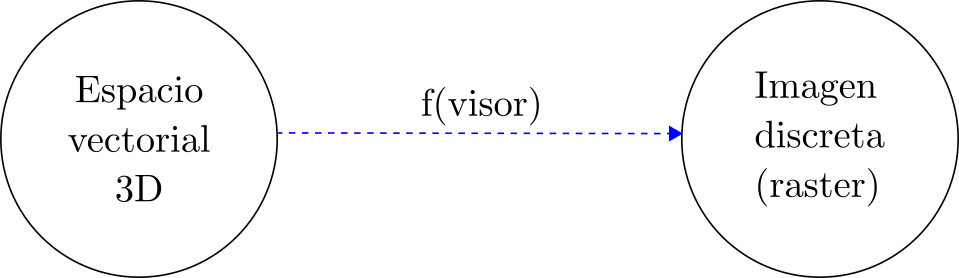
\includegraphics[width=8cm]{Img/CPD/grafica3.png}
\centering
\caption{\footnotesize{Esquema de visualización.}}
\label{fig:grafica3}
\end{figure}


La visualización se logra mediante una secuencia de operaciones conocida como \textit{viewing pipeline} \citep{marsh2005applied} ilustrada en la figura \ref{fig:view0}. En primer lugar, se aplica una proyección que mapea el objeto 3D a un nuevo objeto ``plano'' en un \textbf{plano de visión} en inglés \textit{Viewplain}.
Luego, se define un sistema de coordenadas en el viewplane especificando un punto como origen, y dos vectores perpendiculares que dan las direcciones de los ejes de coordenadas. Se aplica una asignación de coordenadas del viewplane para expresar el objeto ``plano'' en términos del sistema de coordenadas del plano bidimensional elegido. Finalmente, el objeto ``plano'' se asigna a la pantalla del dispositivo por medio de una transformación de coordenadas bidimensional \citep{marsh2005applied}. 

\begin{figure}[ht]
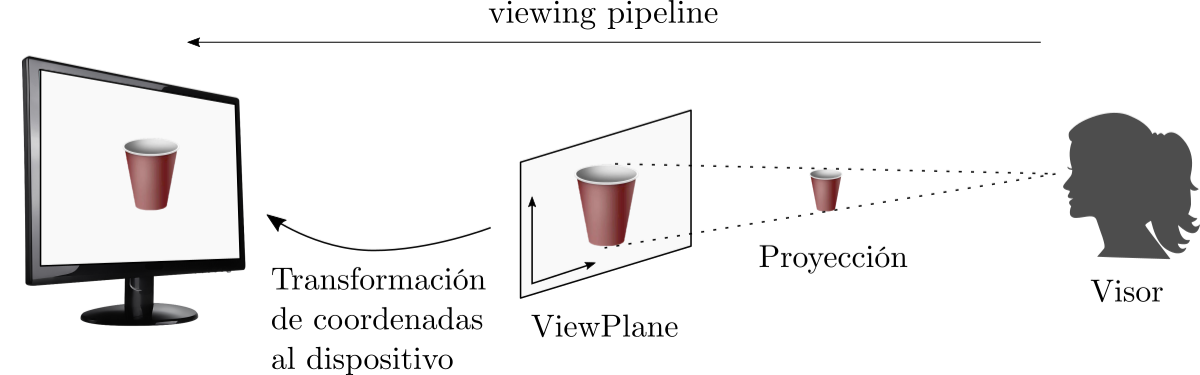
\includegraphics[width=13cm]{Img/GEO/geo-view001.png}
\centering
\caption{\footnotesize{Secuencia de operaciones para la visualización (\textit{viewing pipeline}). }}
\label{fig:view0}
\end{figure}


Básicamente hay dos métodos para proyectar objetos tridimensionales sobre una superficie bidimensional:  \textbf{proyección en perspectiva} y \textbf{proyección en paralelo}. 

Sea $n$ el vector plano de un viewplane, y sea $V$ (punto de visión o cámara) un punto que no está sobre el viewplane. La proyección en perspectiva de $V$ sobre $n$ es la transformación que mapea cualquier punto $P$ del objeto, distinto de $V$, en el punto $P^{\prime}$ que es la intersección de la línea $\overline{VP}$ y el plano $n$, como se ilustra en figura \ref{geo-view1} (a). La proyección se efectúa mediante líneas que convergen en una posición determinada.
Si $V$ es un punto en el infinito, la proyección es paralela, todos los puntos del objeto se proyectan sobre la superficie bidimensional mediante líneas paralelas (ver figura \ref{geo-view1} (b)) \citep{marsh2005applied}.

\begin{figure}[h]
    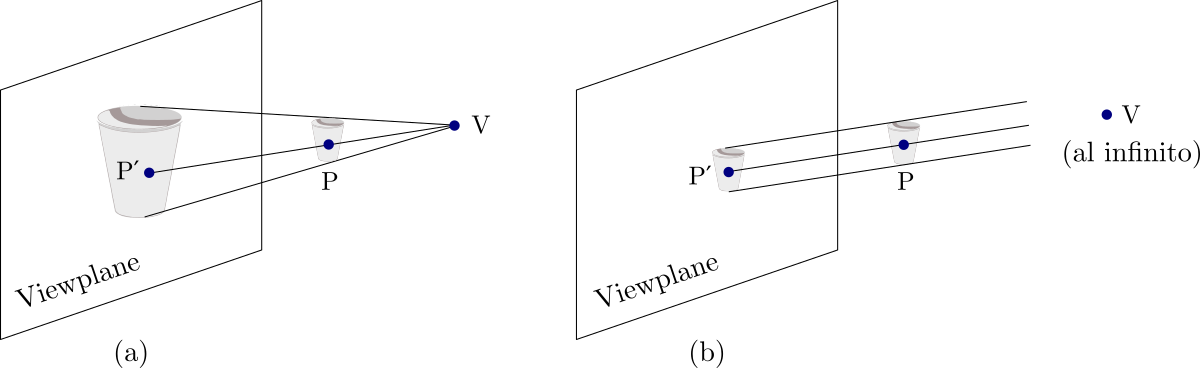
\includegraphics[width=14cm]{Img/GEO/geo-view11.png}
    \centering
    \caption{\footnotesize{Proyección en perspectiva y Proyección en paralelo.}}
    \label{geo-view1}
\end{figure}

La proyección desde el punto de visión $V$ al viewplane $n$ es una transformación tridimensional dada por la siguiente matriz \citep{marsh2005applied} (ver ecuación \ref{eq:4}):

\begin{equation}
M = n^TV - (n  · V)I_4
\label{eq:4}
\end{equation}

Siendo $I_4$ una matriz identidad de 4x4.

\vspace{5mm}

Las tecnologías de visualización implementan estos conceptos de diferentes maneras dependiendo del contexto en que se utilizan, por ejemplo, en \Gls{OpenGL}\footnote{\url{https://www.opengl.org/}} se implementa la visualización mediante las matrices Modelo, Vista y Proyección en inglés \textit{model-view-projection matrix} \citep{kessenich2016opengl}.

En el diseño CAD es fundamental que los modelos estén bien definidos (consistentes) y la visualización es auxiliar (aunque necesaria), por lo que no tiene demasiada importancia la resolución\footnote{La resolución de una imagen indica la cantidad de detalles que puede observarse en esta. } de las imágenes, al menos en las primeras fases de diseño.\newline




\subsection{Diseño de Objetos} 
\label{sectionDisenoObjetos}
\label{disGeo}

Los modelos sólidos se pueden diseñar mediante el \textbf{modelado poligonal} \citep{russo2010polygonal} que consta en la manipulación de vértices, aristas o caras de los poliedros. Este enfoque es muy  flexible porque los ordenadores pueden renderizar los modelos muy rápido, sin embargo, al contener polígonos planos se dificulta la cobertura geométrica al construir modelos de geometría compleja, por ejemplo: para generar superficies curvas precisas se necesitan grandes cantidades de polígonos. Para solventar ese problema se utilizan otras técnicas de modelado, incluyendo:

\subsubsection{Modelado Booleano (CSG) }
\label{mod:booleano}
Al conjunto de procesos que permiten el diseño de sólidos complejos mediante la combinación booleana de objetos simples (primitivas) se conoce como \textbf{modelado booleano}, o también  \textbf{Geometría Constructiva de Sólidos} en inglés \textit{Constructive Solid Geometry} (\Gls{CSG}) \citep{foley1996computer}.\newline
En el modelado booleano, luego de escalar, trasladar y rotar convenientemente las primitivas, se aplican los operadores booleanos regularizados  ($\cup^*$, $\cap^*$ y $-^*$) para combinarlas. Un sólido construido mediante un modelador booleano (CSG) queda descrito mediante un árbol binario en el que:

\begin{itemize}
\item El nodo raíz es el sólido resultante.
\item Los nodos internos son los operadores booleanos.
\item Los nodos hoja son las primitivas.
\end{itemize}

En los nodos terminales del árbol no sólo se representan las primitivas, sino que también se indican las transformaciones lineales que se han de efectuar sobre ellas. En el árbol, tanto las operaciones como los nodos hoja deberán encontrarse ordenadas, debido a que las operaciones booleanas no son, en general, conmutativas. El proceso de seguimiento (recorrido) del árbol se hará partiendo de los nodos terminales.



En el ejemplo de la figura \ref{fig:bool} se puede ver la descripción de un modelo booleano  llamado $R_3$ como un árbol CSG utilizando las operaciones booleanas: unión ($\cup$), intersección ($\cap$) y diferencia ($-$) \citep{Wassermann_2016}.

\begin{figure}[ht]
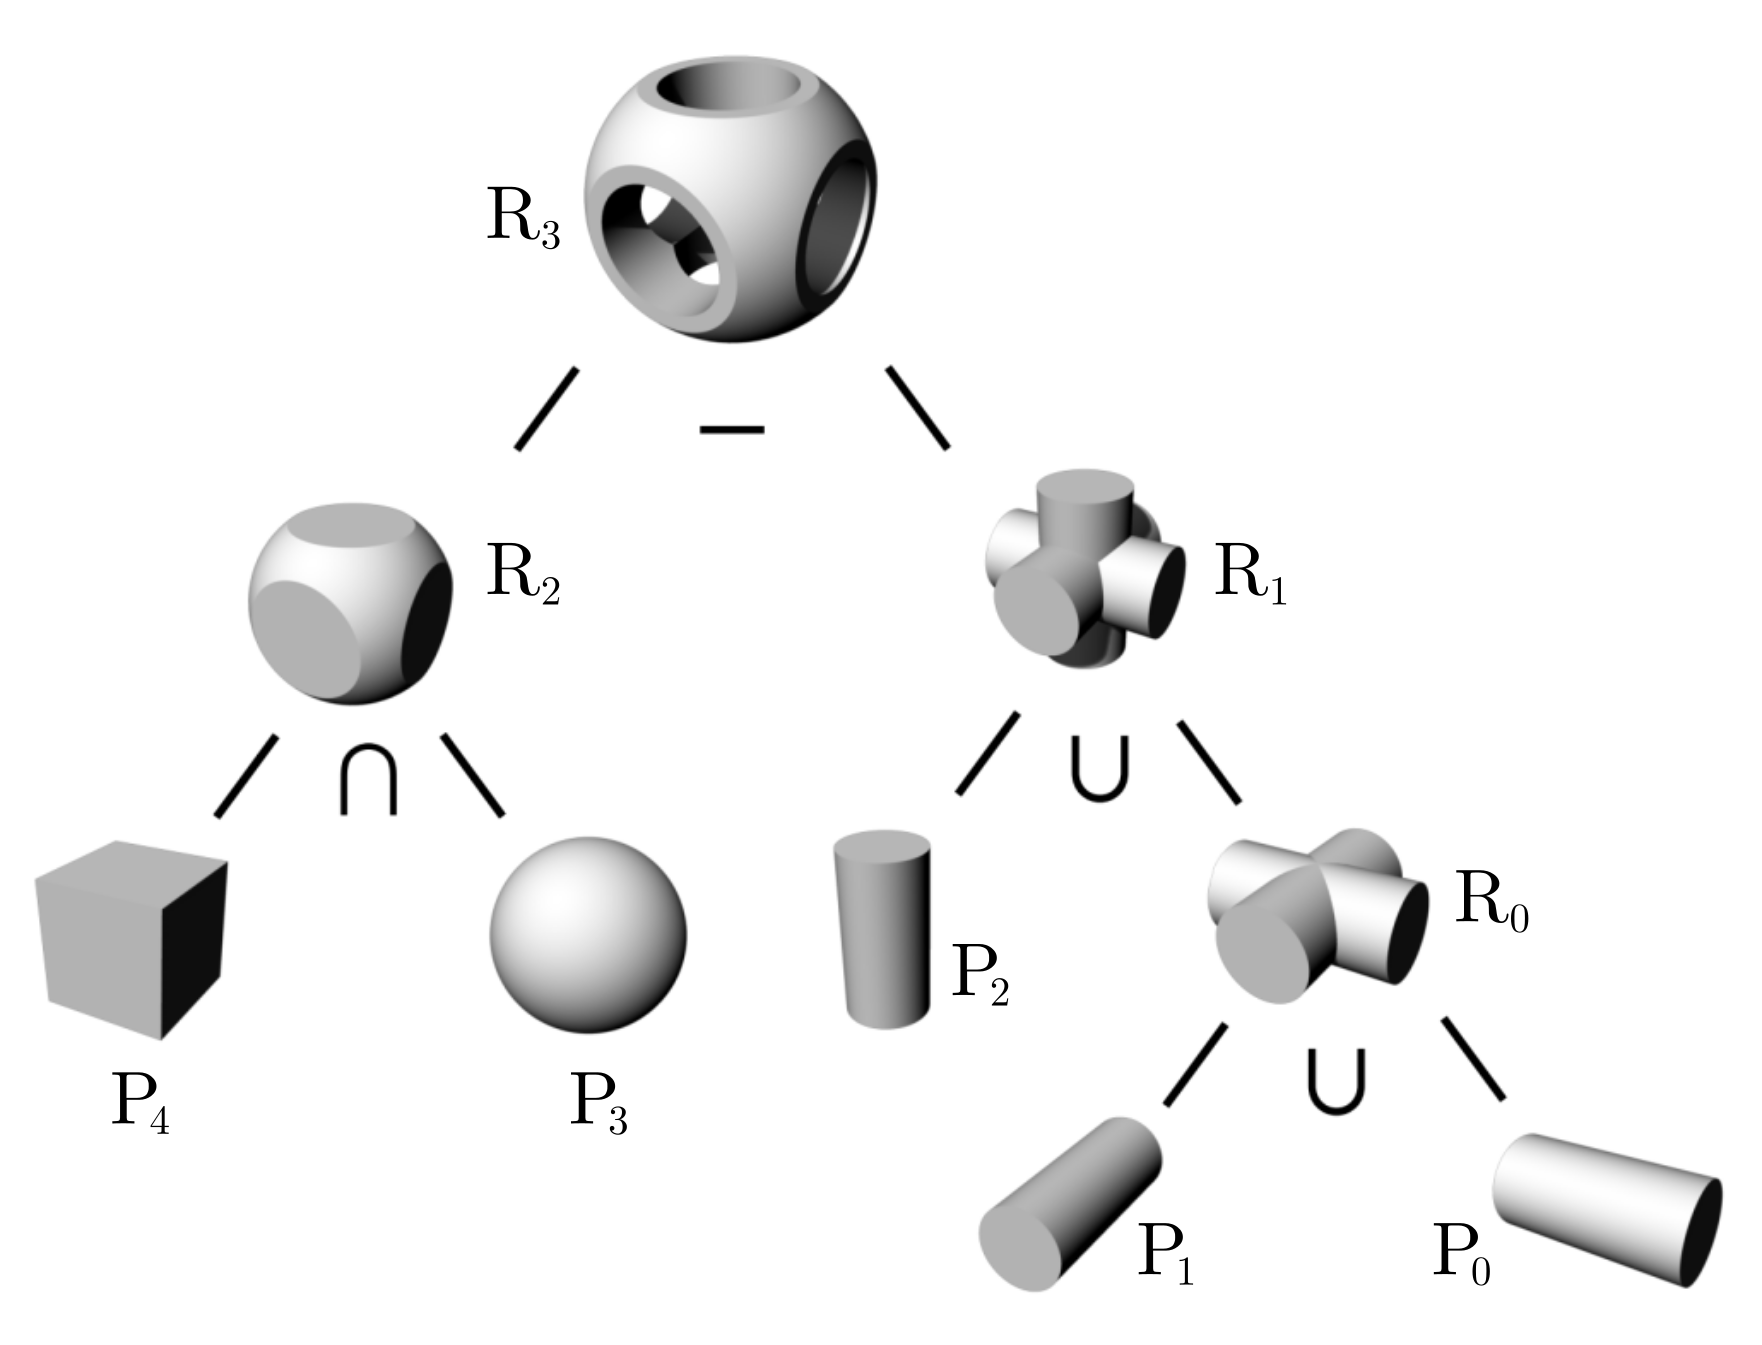
\includegraphics[width=10cm]{Img/GEO/geo-booleano6.png}
\centering
\caption{\footnotesize{Árbol CSG utilizando las   operaciones booleanas: unión ($\cup$), intersección ($\cap$) y diferencia ($-$). %En la derecha se observa que $R_0$ es la unión de los cilindros $P_0$ y $P_1$ mediante la ecuación ($R_0 = P_0\cdot T_0 \cup P_1\cdot T_1$), luego se efectúa la unión entre $R_0$ y el cilindro $P_2$ dando como resultado $R_1$ mediante ($R_1 = R_0 \cup P_2\cdot T_2$). Por su parte en la izquierda $R_2$ es la intersección entre la esfera $P_3$ y el cubo $P_4$ $R_2 = P_3\cdot T_3 \cap P_4\cdot T_4$. Finalmente el nodo raíz resultante $R_3$ es la diferencia entre $R_2$ y $R_1$ mediante ($R_3 = R_2 - R_1$). También se aprecia un transformación de escala en la figura resultante, aumentando su tamaño, esto se debe a la aplicación de las matrices de transformación $T$ en cada operación \citep{Wassermann_2016}.
}}
\label{fig:bool}
\end{figure}


Partiendo de las primitivas $P_0$ (cilindro), $P_1$ (cilindro), $P_2$ (cilindro), $P_3$ (esfera) y $P_4$ (cubo) se obtiene el objeto final ($R_3$) después de tres niveles de operaciones booleanas.\vskip
En primer lugar se efectúa la unión de $P_0$ y $P_1$, después de haber transformado y posicionado adecuadamente las primitivas en el espacio, mediante las matrices netas $T_0$ y $T_1$ (ver ecuación \ref{eq:5}).

\begin{equation}
R_0 = P_0\cdot T_0 \cup P_1\cdot T_1
\label{eq:5}
\end{equation}

A continuación el resultado intermedio $R_0$ se suma con la primitiva $P_2$ (cilindro), después de haber sido escalada y posicionada por $T_2$ (ver ecuación \ref{eq:6}).

\begin{equation}
R_1 = R_0 \cup P_2\cdot T_2
\label{eq:6}
\end{equation}

Para producir el resultado $R_2$ se realiza la intersección entre $P_3$ y $P_4$, después de haber transformado y posicionado adecuadamente las primitivas en el espacio, mediante las matrices netas $T_3$ y $T_4$ (ver ecuación \ref{eq:8}).

\begin{equation}
R_2 = P_3\cdot T_3 \cap P_4\cdot T_4
\label{eq:8}
\end{equation}

Finalmente, a $R_2$ se le resta $R_1$, obteniendo así el objeto raíz del árbol $R_3$ (ver ecuación \ref{eq:9}).


\begin{equation}
R_3 = R_2 - R_1 = (P_3\cdot T_3 \cap P_4\cdot T_4) - ((P_0\cdot T_0 \cup P_1\cdot T_1) \cup (P_2\cdot T_2))
\label{eq:9}
\end{equation}

En el ejemplo se puede apreciar que las transformaciones han incrementado el tamaño del sólido resultante $R_3$. Por lo general, el escalado de las primitivas no es uniforme, es decir, los factores de escala $s_x$, $s_y$, y $s_z$ son diferentes. De este modo, una sola primitiva puede proporcionar una gran variedad de copias diferentes simplemente usando transformaciones. \vskip
Es importante indicar que el modelado booleano es un proceso descriptivo, es decir, sólo se limita a especificar qué primitivas se utilizan y cómo se combinan. De manera que sólo se dispone de la información geométrica y topológica de las primitivas pero no la de los objetos resultantes. Para poder combinar las primitivas en un esquema de modelado, éstas han de ser definidas previamente. Una forma frecuente de crearlas es estableciendo los parámetros de las ecuaciones que las definen. 


%\clearpage
\subsubsection{Diseño de nuevas primitivas}
La figura \ref{fig:csg3} muestra dos primitivas con los parámetros de control que cada una requiere (excluidos los de posición y orientación). A la izquierda un cono con 2 parámetros: altura ($H$) y radio ($R$). A la derecha un cono truncado con 3 parámetros: altura ($H$), radio superior ($R1$) y radio inferior ($R2$). La primitiva de la izquierda en 3D solo puede generar conos. La primitiva de la  derecha por su parte puede generar cilindros, conos y conos truncados. 
\citep{Ramos2011}. 
Cuanto más flexible es esta definición, mayor es la capacidad para modelar los diferentes objetos y por consecuencia mayores son las posibilidades de modelado. Se llama dominio o \textbf{poder expresivo} de un modelador, a la capacidad que posee para modelar los diferentes objetos. %Cuanto mayor sea el poder expresivo de un modelador, mayores son las posibilidades de modelado. 

\begin{figure}[ht]
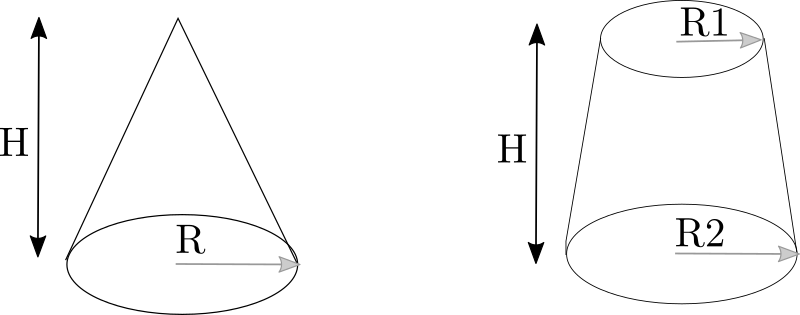
\includegraphics[width=6cm]{Img/GEO/geo-cono.png}
\centering
\caption{\footnotesize{Primitivas con sus parámetros de control.}}
\label{fig:csg3}
\end{figure}


%Un sistema de modelado permite al usuario definir sus propias primitivas y así aumentar el dominio y la potencia del modelador. 
%En la generación de nuevas ejemplares, 
El sistema de modelado define un conjunto objetos sólidos que son relevantes para un área de aplicación determinada. Estos suelen parametrizarse no sólo en función de las transformaciones, sino también con base a otras propiedades. Por ejemplo, objetos como engranajes o tuercas son tediosos de definir utilizando combinaciones booleanas de objetos más sencillos pero pueden ser formulados fácilmente con parámetros de alto nivel como diámetro, espesor, número de dientes, etc. (Ver figura \ref{fig:csg4}). El cambio en los parámetros genera objetos con diferentes características, por ejemplo: el engranaje de la derecha no posee ningún orificio, producto del cambio de valor $Radio \ de \ orificio = 0$.


\newline


\begin{figure}[h]
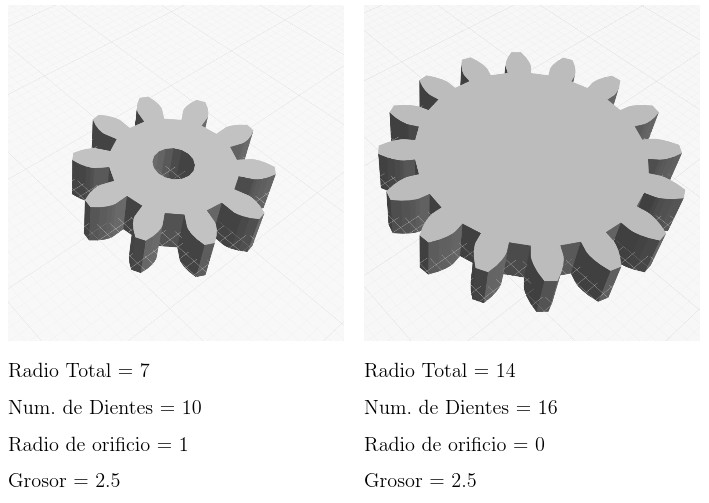
\includegraphics[width=12cm]{Img/Modelos/engranaje.jpg}
\centering
\caption{\footnotesize{Dos engranajes generados a partir de la misma primitiva.}}
\label{fig:csg4}
\end{figure}

La única forma de modelar un nuevo tipo de objeto es describiendo el mecanismo que lo define, es decir, es necesario escribir las rutinas o programas que lo dibujan o determinan sus propiedades.





\section{Sistemas CAD}
Para comprender el estado actual del CAD primero se deben estudiar algunas aplicaciones disponibles. 
Las soluciones presentadas incluyen herramientas basadas en el escritorio y basadas en la web. A continuación se describen las características más relevantes para este trabajo: Permitir el diseño paramétrico, contar con interfaz de \textit{scripting} y proveer mecanismos para generar modelos sólidos.


\subsubsection{Blender} 
\textbf{\Gls{Blender}} \citep{BlenderFoundation} es una una suite de creación 3D FLOSS compatible con la totalidad del trabajo en 3D: modelado, rigging, animación, simulación, renderizado, composición y tracking de movimiento, incluso edición de video y creación de videojuegos. Está principalmente orientada a producciones artísticas, sin embargo, dispone de herramientas y primitivas para generar sólidos orientados a la fabricación digital. También permite el uso de modificadores que son operaciones automáticas que afectan a un objeto de una manera no destructiva\footnote{ No destructivo se refiere a hecho de realizar cambios sin sobrescribir los datos del modelo original, de manera que se puedan revertir.}. Con los modificadores, se pueden realizar tareas que manualmente serían demasiado tediosas. Entre muchos otros, se encuentra el modificador booleano que valga la redundancia se utiliza para  operaciones booleanas entre objetos. Otra capacidad de  Blender es el acceso a su \Gls{API}\footnote{\url{https://docs.blender.org/api/current/}} mediante \textit{scripting}, utilizando el lenguaje de programación python\footnote{\url{https://www.python.org/}}.\\
En la figura \ref{fig:blenda} se puede ver la interfaz de Blender y la aplicación de intersecciones mediante el modificador booleano, también se aprecia el código en python para realizar la misma operación mediante su API \citep{blenderBoolean}.


\begin{figure}[h]
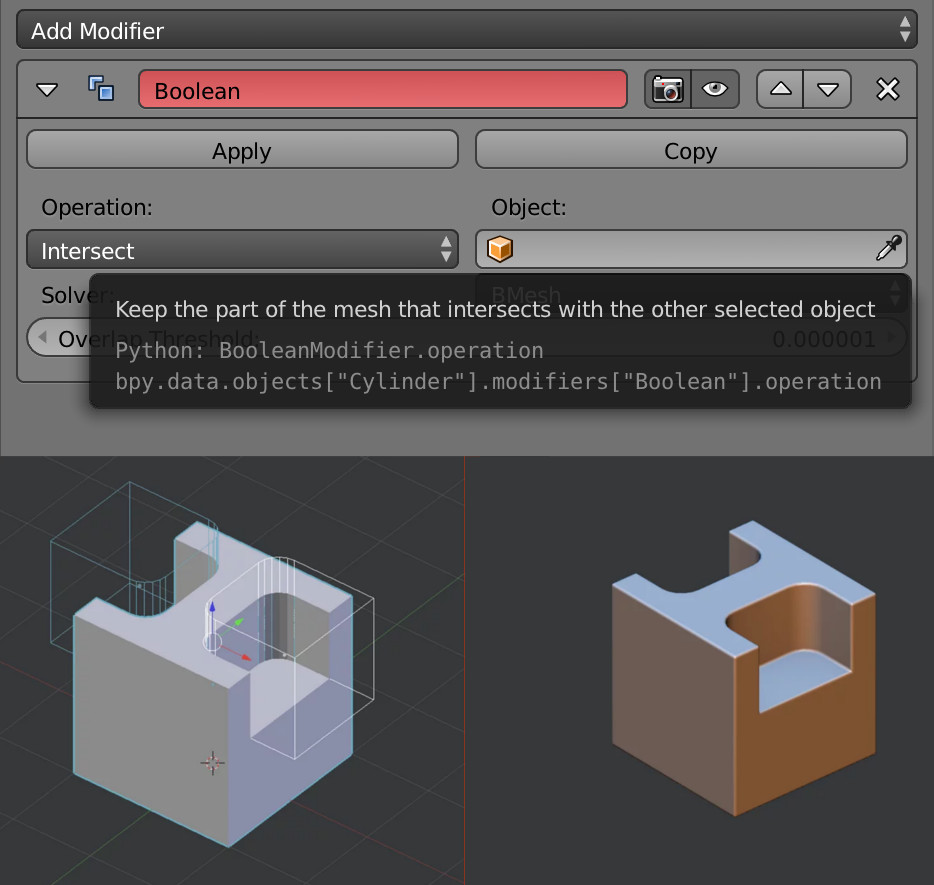
\includegraphics[width=8cm]{Img/Modelos/modelado22.jpg}
\centering
\caption{\footnotesize{Modificador booleano de Blender}. }
\label{fig:blenda}
\end{figure}


\subsubsection{Grasshopper} 
En la última década se ha visto la aparición de un nuevo tipo de interfaz visual para \textit{scripting}. Este tipo de programación visual implica representar programas no como texto, sino como diagramas. Un ejemplo de estas aplicaciones es \textbf{\Gls{Grasshopper}} \citep{BobMcNeel}, un editor de algoritmos gráficos estrechamente integrado con las herramientas de modelado 3D de \Gls{Rhino}\footnote{\url{https://www.rhino3d.com/}}. Se basa principalmente en nodos que mapean el flujo de relaciones desde parámetros, a través de funciones definidas por el usuario, concluyendo normalmente con la generación de geometrías. Las modificaciones en los parámetros o las relaciones del modelo hacen que los cambios se propaguen a través de las funciones explícitas para volver a dibujar la geometría automáticamente. Esta es otra forma de crear modelos paramétricos.

En la figura \ref{fig:grass} se muestra un programa en Grasshopper en forma de diagrama y las relaciones entre los nodos (derecha). A la izquierda se aprecia el modelo resultante en e visor 3D de Rhinoceros \citep{DanielParametric}.

\begin{figure}[h]
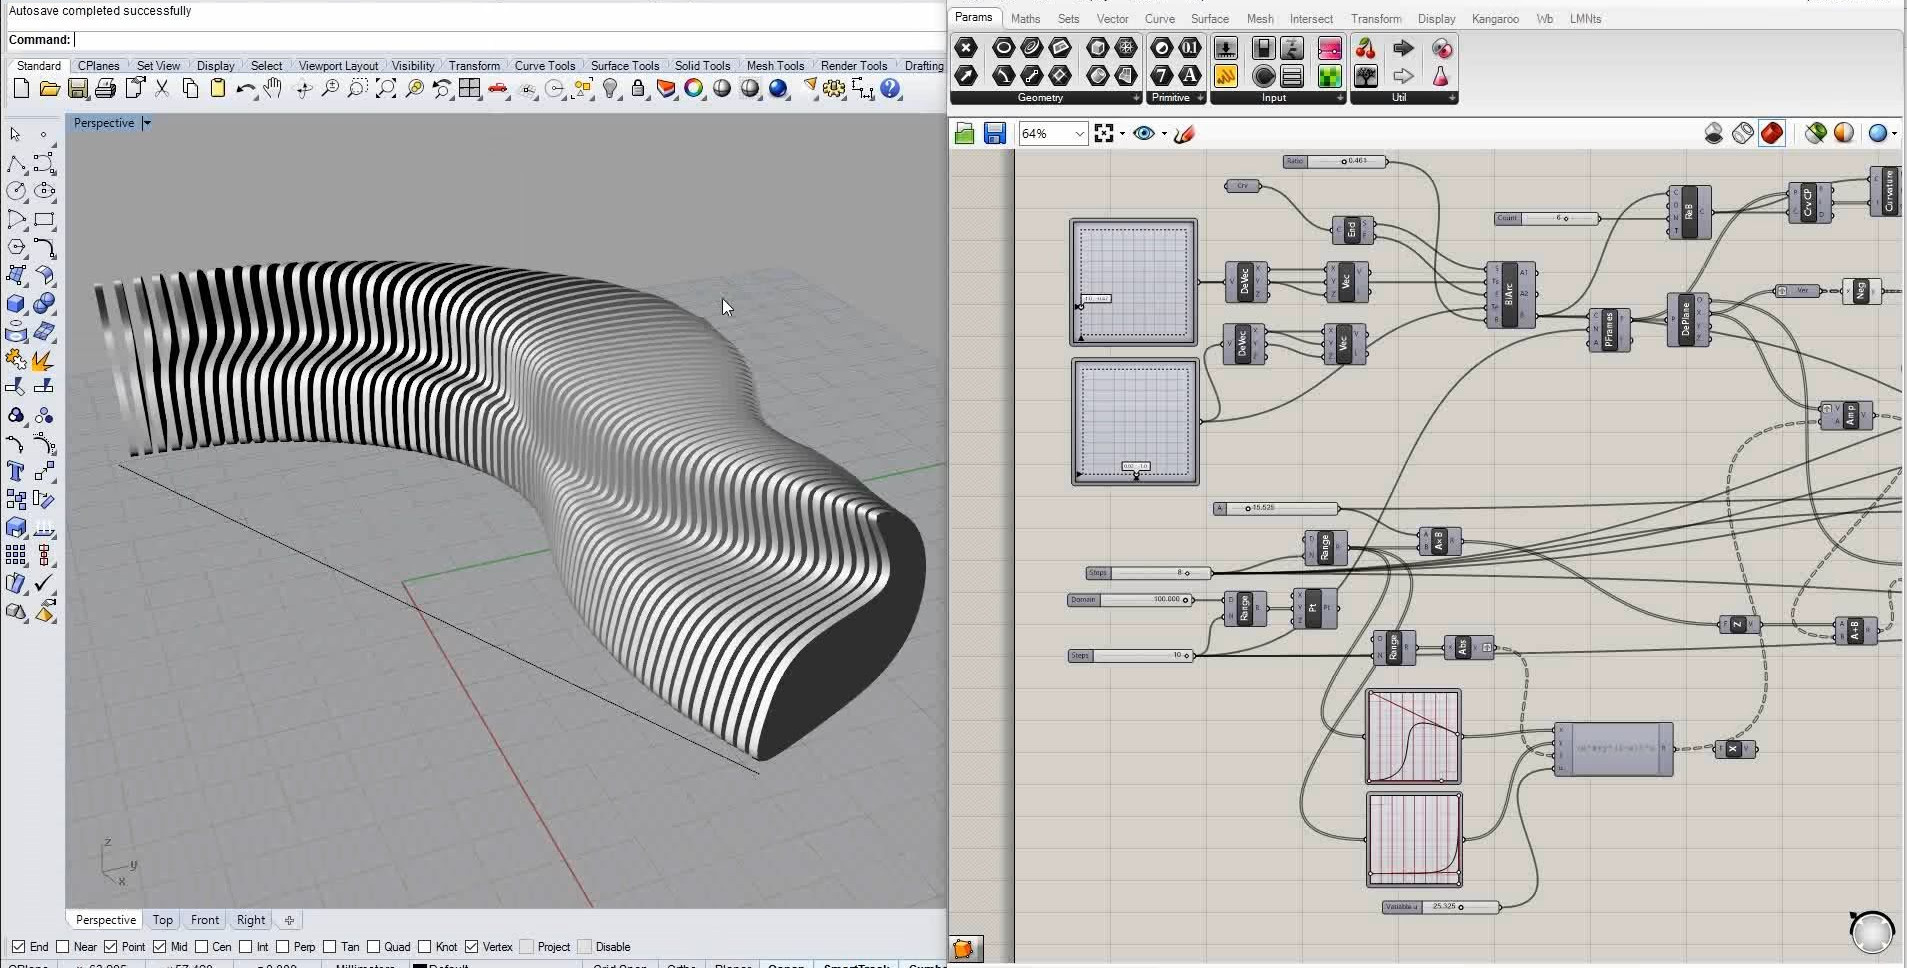
\includegraphics[width=14cm]{Img/CPD/cpd-grass.jpg}
\centering
\caption{\footnotesize{Programa en Grasshopper.}}
\label{fig:grass}
\end{figure}


\subsubsection{OpenJSCAD} 
\textbf{\Gls{OpenJSCAD}}\footnote{\url{http://openjscad.org/}} está inspirado en \Gls{OpenSCAD}\footnote{\url{http://openscad.org/}} y esencialmente proporciona un enfoque a programadores para desarrollar modelos mediante una interfaz web. El diseño paramétrico se realiza mediante scripts en código \Gls{JavaScript} \citep{flanagan2007javascript}, utilizando  funciones \textbf{CSG} y otras un tanto especiales, proporcionadas por el mismo entorno.
Permite incorporar parámetros en la interfaz gráfica, posibilitando al usuario cambiar los  valores de forma interactiva. Utiliza otras librerías como base para cumplir con sus funcionalidades. Para modelado booleano requiere de \textbf{\Gls{CSG.js}}\footnote{\url{https://github.com/jscad/csg.js}} y para la visualización de los modelos 3D  utiliza \textbf{\gls{lightgl.js}}\footnote{\url{https://github.com/evanw/lightgl.js/}} que facilita el desarrollo de aplicaciones WebGL, re-implementando la matriz modelo-vista/proyección\footnote{\url{http://www.opengl-tutorial.org/es/beginners-tutorials/tutorial-3-matrices/}} (analizada en   la sección \ref{visGeo}) de OpenGL\footnote{\url{https://www.opengl.org/}}. 

En la figura \ref{fig:openjscad} se puede ver a la izquierda el modelo 3D de un engranaje y los campos con sus parámetros. A la derecha se sitúa el editor de texto con el programa correspondiente escrito en JavaScript \citep{openJSCADorg}.

\begin{figure}[h]
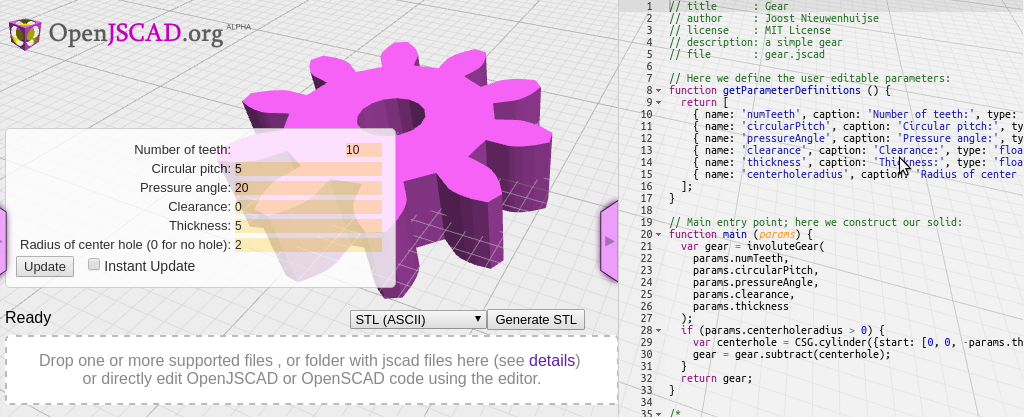
\includegraphics[width=14cm]{Img/openjscad-params.png}
\centering
\caption{\footnotesize{
Interfaz de OpenJSCAD.
}}
\label{fig:openjscad}
\end{figure}



\subsubsection{OnShape} 
\textbf{\Gls{OnShape}}\footnote{\url{https://www.onshape.com/}} (ver figura \ref{fig:onshape}) \citep{OnshapePlanes} es una aplicación CAD basada en la nube que puede ser accedida desde cualquier navegador o mediante una aplicación para móviles. Su dominio esta fuertemente orientado al \textbf{diseño mecánico} \citep{lardies2012criterios} con características similares a programas como \Gls{SolidWorks}\footnote{\url{https://www.solidworks.com/es}}. 
Cuenta con un sistema de control de versiones\footnote{Se llama control de versiones a la gestión de los diversos cambios que se realizan sobre los elementos de algún producto o una configuración del mismo} para los documentos del proyecto (dibujos, modelos 3D y documentos) y soporta la colaboración en tiempo real. La aproximación de modelado es de manipulación directa, sin embargo, incluye un lenguaje de \textit{scripting} que se denomina \Gls{FeatureScript}\footnote{\url{https://cad.onshape.com/FsDoc/}} y permite la definición de la geometría, relaciones y parámetros para la construcción de modelos 3D Paramétricos \citep{Alfaiate2017}.

\begin{figure}[h]
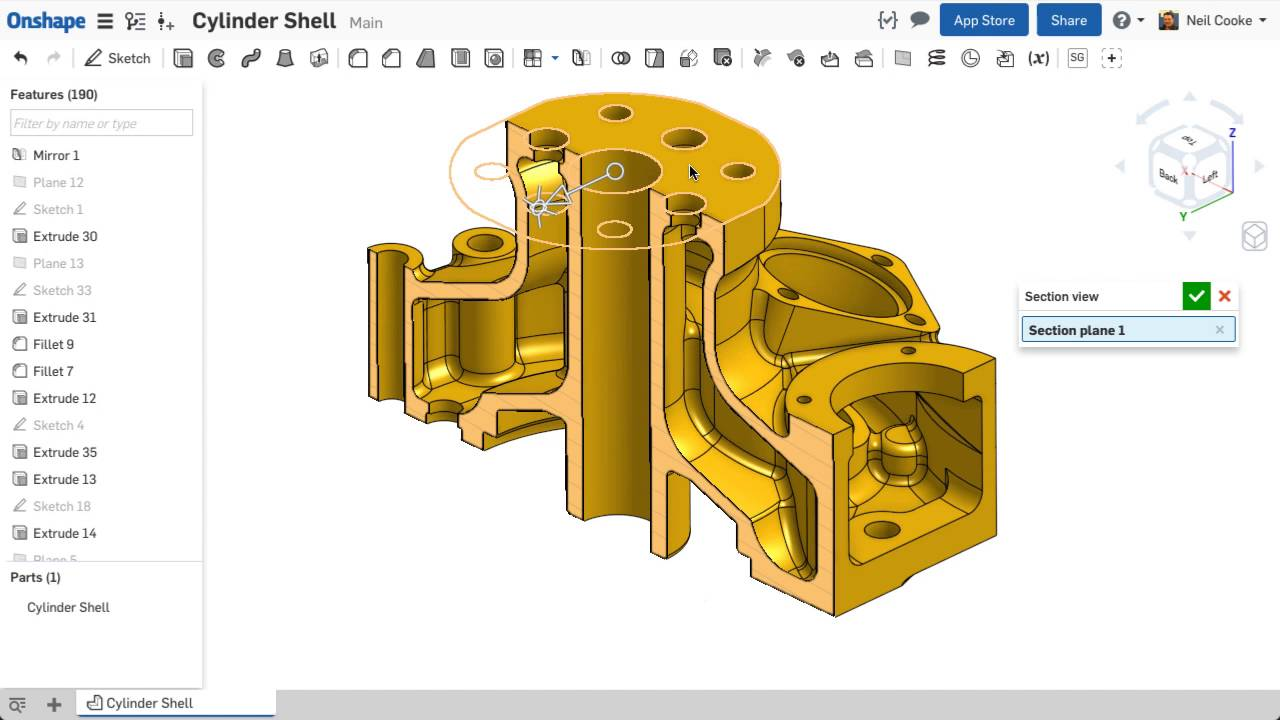
\includegraphics[width=14cm]{Img/onshape.jpg}
\centering
\caption{\footnotesize{Interfaz de OnShape.}}
\label{fig:onshape}
\end{figure}

\cleardoublepage
\chapter{{Desarrollo Colaborativo de Productos CAD con Lean UX}}
\label{chap:cap3}

En este capítulo se explican los conceptos que involucran el desarrollo de los sistemas colaborativos y distribuidos para CAD y la metodología \textit{Lean UX} como una herramienta de soporte para desarrollar un software con tales características. Finalmente se describen algunos ejemplos de aplicaciones CAD colaborativas y distribuidas disponibles en la web.\vskip 0mm

\section{Introducción}
La complejidad creciente de los productos hace necesaria 
la colaboración entre diferentes personas, habitualmente se generalizan  en ``cliente'' y ``diseñador'' a las partes que interactúan, pero no necesariamente son una única persona por cada parte, 
sino equipos conformados por múltiples roles. Sus diferentes habilidades pueden abarcar el modelado 3D, la producción física con diferentes tecnologías (impresión 3D, corte a láser, control numérico, etc.), el marketing, etc. \vskip  

Tradicionalmente, la interacción se producía entregando los planos a  ``contratistas'' para que construyan las distintas partes que integran un proyecto, los contactos se producían de forma presencial y obligaban a frecuentes viajes para mantener el proyecto bajo control \citep{Ruiz}. Esta modalidad de trabajo se caracteriza por utilizar un \textbf{modelo en cascada}, que ordena rigurosamente las etapas del ciclo de vida de un proyecto, de tal forma que el inicio de cada etapa debe esperar a la finalización de la  anterior \citep{de2001metodologia}. Este modelo tiene la ventaja de ser sencillo de comprender e implementar, ya que se sabe de antemano que esperar del proyecto, con una estimación precisa del costo y  duración.
Sin embargo, una vez que un producto se encuentra en la etapa de prueba o revisión, es muy difícil realizar algún cambio por algo que no fue definido adecuadamente. De modo que el riesgo y la incertidumbre son elevados en los proyectos donde los requerimientos cambian constantemente. Por otro lado, no se distingue en involucrar al usuario final o cliente durante el proceso, si se solicita algún cambio no previsto, el proyecto se puede retrasar y salirse del presupuesto.\vskip
El avance de las tecnologías web ha democratizado la participación en los procesos de diseño en muchos niveles. Los teléfonos inteligentes son un ejemplo de la tecnología al servicio de las personas, porque ofrecen oportunidades para la co-creación mediante sus aplicaciones \citep{Huerta2013}. En consecuencia, el rol del contratista tradicional ha cambiado y esto implica que realice su trabajo en estrecha relación con otros actores, en colaboración y  sin necesidad del contacto presencial. En este nuevo escenario, la aparición de conceptos como \textbf{Desarrollo Colaborativo de Productos} en inglés \textit{Collaborative Product Development} (CPD) \citep{Elfving2007} impulsan la participación de ingenieros, diseñadores industriales, arquitectos, programadores, artistas e incluso personas sin formación específica en procesos conocidos como \textbf{co-diseño} o \textbf{diseño colaborativo}.

\section{Co-diseño}
 Se entiende como \textbf{co-diseño} al  proceso de colaboración creativa entre diseñadores y otras personas, las cuáles no poseen una formación previa en diseño, con el propósito de resolver problemas  \citep{PerezGarcia2014}.  
 En esta definición se plantean dos elementos fundamentales que dan soporte al paradigma colaborativo:
\begin{enumerate}
    \item \textbf{Nuevos perfiles}: Al grupo habitual de trabajo se suman la iniciativa y la creatividad de otros perfiles que antes aportaban ideas generalmente como agentes externos: el investigador y el usuario final. Estos perfiles tienden a mezclarse: El usuario pasa a jugar un rol de ``experto en su experiencia'' y puede aportar elementos de valor en la generación de conceptos e ideas en la etapa inicial del proyecto. El investigador, a partir de la experiencia del usuario, puede  recoger todos los datos y, a la vez, desempeñar un papel fundamental en formalizar las ideas. Lógicamente, una misma persona puede cumplir más de un rol y el diseñador debe cambiar al incluir nuevos ``socios creativos'' en un entorno que tradicionalmente le pertenecía.\vskip
\item \textbf{Objetivo en común}: La idea del \textbf{objetivo compartido} se plantea como una de las principales diferencias con respecto a los métodos tradicionales. Los métodos de diseño generalmente se planteaban para ser llevados a cabo solamente por expertos que realizaban tareas individuales y no era necesario compartir la visión del objetivo general del proceso. En cambio, en un proyecto colaborativo este punto es fundamental: Para que el equipo funcione correctamente necesita tener la visión del objetivo en común \citep{Huerta2013}.

\end{enumerate}


En la figura \ref{fig:codesign} se pueden apreciar las diferencias entre un esquema de \textbf{diseño tradicional vs co-diseño} \citep{Sanders2008}. En el esquema de la izquierda (tradicional) los roles trabajan por separado, el investigador aporta conocimientos para realizar la lista de requerimientos de diseño, la interacción del diseñador (contratista) con el usuario es a través de dicha lista. De esa manera el diseñador trabaja en base a los requerimientos y una vez finalizado todo el trabajo recién se efectúa la entrega. \vskip
Por otra parte, en el esquema de la derecha (co-diseño) el usuario participa durante todo el proceso de diseño a través de la  interacción directa con todo el equipo, en este ejemplo, el contratista cumple el rol de diseñador e investigador. La  interacción se realiza mediante las herramientas inherentes a cada proyecto, que pueden ser diagramas, referencias, artefactos, métodos y/o técnicas. En lugar de establecer los requerimientos, se plantean las necesidades de diseño y las entregas del trabajo se realizan progresivamente mediante la revisión continua del producto por parte de todos los participantes. 


\begin{figure}[h]
\centering
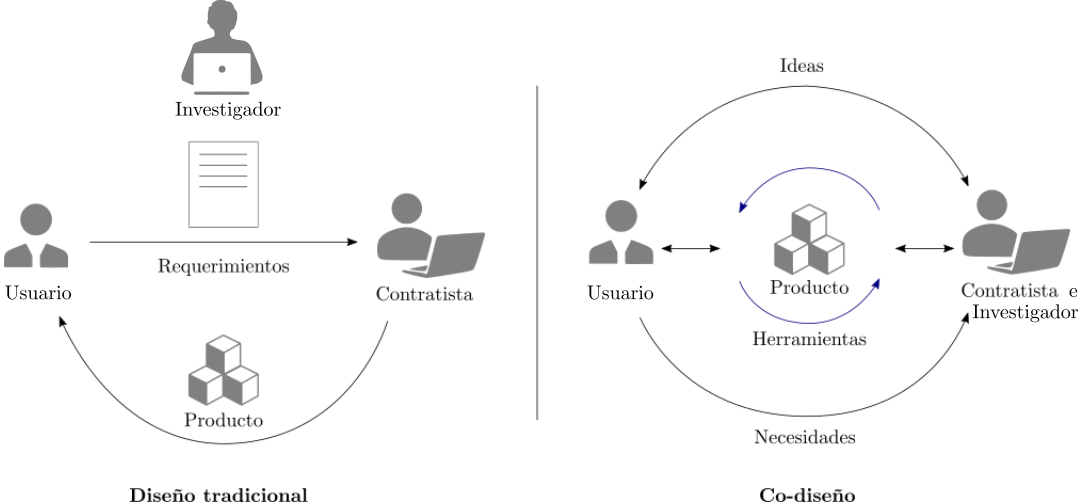
\includegraphics[width=16cm]{Img/INTRO/intro-codesign0.png}
\caption{\footnotesize{Diseño tradicional vs co-diseño.}}
\label{fig:codesign}
\end{figure}


La diversidad de profesiones en el co-diseño trae como consecuencia que los actores difieran tanto en la forma de interpretar el diseño como en la forma de comunicarlo. Generalmente la comunicación está cargada de jerga propia de cada especialidad y por lo tanto, es difícil de comprender para los demás participantes. Aun así, si se comprendieran las palabras, el significado de las mismas puede diferir según la disciplina. Un ejemplo de palabra con muchos significados es \textit{``concepto''}, la figura \ref{fig:concept} muestra cómo los actores de diferentes especialidades interpretan de diferente manera la misma palabra en el ambito de la industria automotriz: 
a) Para un diseñador son los dibujos rápidos, bosquejos o \textit{sketches}. b) Un fabricante de prototipos lo materializa en modelos de arcilla u otro material que permita visualizar rápidamente los detalles del producto, incluso en escala real. c) Para un publicista es la representación digital o render del producto final. d) Un ingeniero mecánico lo entiende en los documentos técnicos, planos y especificaciones. \citep{Kleinsmann2006} \\

En consecuencia, si no se crea un entendimiento compartido sobre el contenido del diseño, se dificulta la colaboración. 

\begin{figure}[ht]
\centering
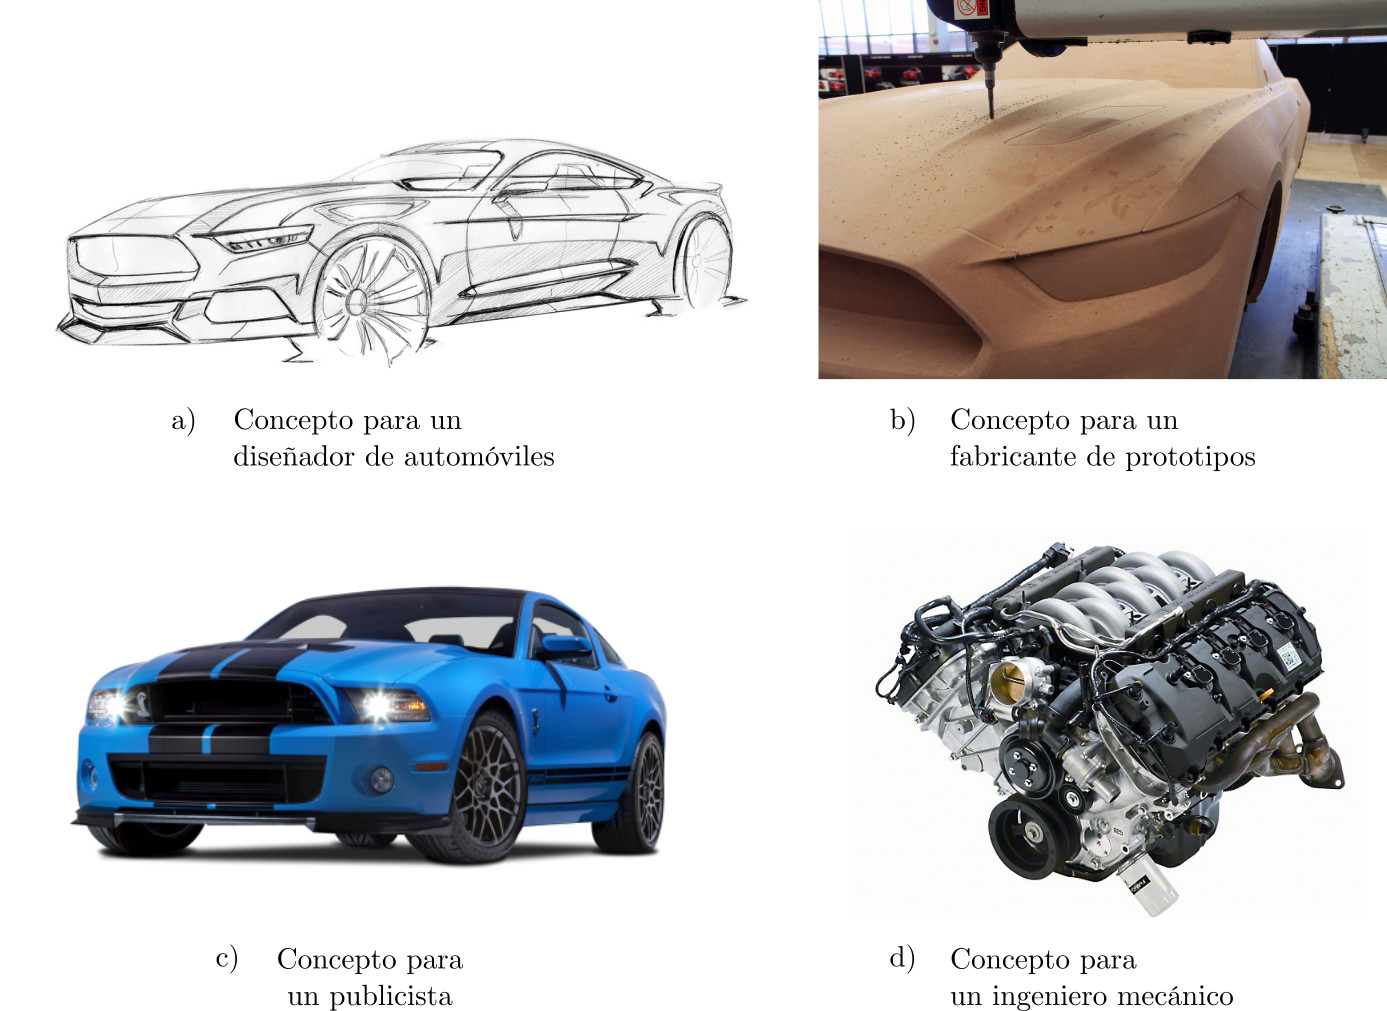
\includegraphics[width=14cm]{Img/INTRO/intro-codesign1.jpg}
\caption{\footnotesize{Interpretación de la palabra ``concepto" según especialistas de la industria automotriz.}}
\label{fig:concept}
\end{figure}

\subsubsection{Diseño Iterativo}
\label{iterativo}

La etapa de \textbf{revisión de los diseños} es fundamental porque permite evaluar la capacidad de los resultados para cumplir los requisitos del cliente, identificar cualquier problema y proponer soluciones \citep{Pereiro2005}. 

Lo más habitual es registrar los resultados de las revisiones en actas de reunión o bien en algún formato que se haya establecido  específicamente para el control. 
Estas tareas parecieran ser anticuadas en términos administrativos, si no se considera que diseñar un objeto tangible implica tener un entendimiento completo de todo lo que se debe hacer antes de iniciar la producción física, porque esta generalmente es compleja comparada con la producción de bienes intangibles. Por lo que la necesidad de la revisión constante y la tendencia creciente a requerimientos que pueden cambiar, ponen en evidencia las limitaciones del modelo en cascada. Como solución surgieron los \textbf{modelos iterativos} que promueven una iteración continua sobre el producto y pruebas a lo largo de todo el proyecto  \citep{laurel2003design}.

El \textbf{diseño iterativo} en inglés \textit{Iterative Design} es una metodología de diseño basada en un proceso cíclico de creación de prototipos\footnote{Un prototipo es un ejemplar o primer molde en que se fabrica una figura u otra cosa.} y pruebas, para analizar y refinar un trabajo que se encuentra en progreso. La interacción con el diseño se utiliza como una herramienta de investigación para recolectar información y desarrollar el proyecto, implementando iteraciones o versiones sucesivas. La prueba, el análisis, el refinamiento y la repetición son necesarios porque la experiencia del usuario no se puede predecir por completo. Las decisiones se basan en la experimentación  con el prototipo, de esta manera el proyecto se desarrolla a través de un continuo diálogo entre los diseñadores, el diseño y el usuario. 

\vskip
En un nivel superficial, el diseño iterativo  difiere del modelo de cascada de una sola manera: en lugar de especificar todo el sistema completo antes de desarrollarlo, se diseña y construye completamente una parte del mismo, y luego se utiliza esa parte y las unidades completadas previamente como base para más diseños y más producción futura. En otras palabras, \textbf{iterar es diseñar} y, específicamente, es comprender el diseño en el momento que se construye el diseño \citep{Chronicles2009}.\vskip




En este punto es necesario hacer una aclaración respecto a otro concepto con el que se suele confundir: \textbf{el diseño incremental} que tiene como objetivo un crecimiento progresivo de la funcionalidad. Es decir, el producto va evolucionando con cada una de las entregas hasta que se adapta a lo requerido por el cliente. Alistair Cockburn describe al enfoque iterativo como ``aprender al completar'' y lo distingue del diseño incremental en el sentido que éste consiste en agregar nuevos elementos, incluso de forma iterativa, mientras que iterar trata sobre volver a trabajar y refinar \citep{cockburn2002agile}. En ocasiones el concepto de iteración se puede perder al reemplazarlo por incrementos, lo que provoca que el proyecto tenga las mismas consecuencias que los en cascada. Jeff Patton, utilizando visualmente el cuadro de la Mona Lisa (ver figura \ref{fig: incremental}) para explicar la diferencia entre los dos métodos \citep{Patton2007}. En el incremental (arriba) se agregan nuevos elementos a partir de una idea completa preconcebida del producto. En el iterativo (abajo) se parte de una idea vaga, ejemplo: ``Una mujer en un ambiente campestre''. De forma iterativa se comienza a trabajar sobre una versión mínima del producto, refinando en cada ciclo hasta llegar a la solución.
Lo más destacado del método iterativo es el siguiente principio subyacente: Hasta que se no se haya construido realmente lo que se está diseñando, no se podrá comprender en su totalidad.

\begin{figure}[ht]
\centering
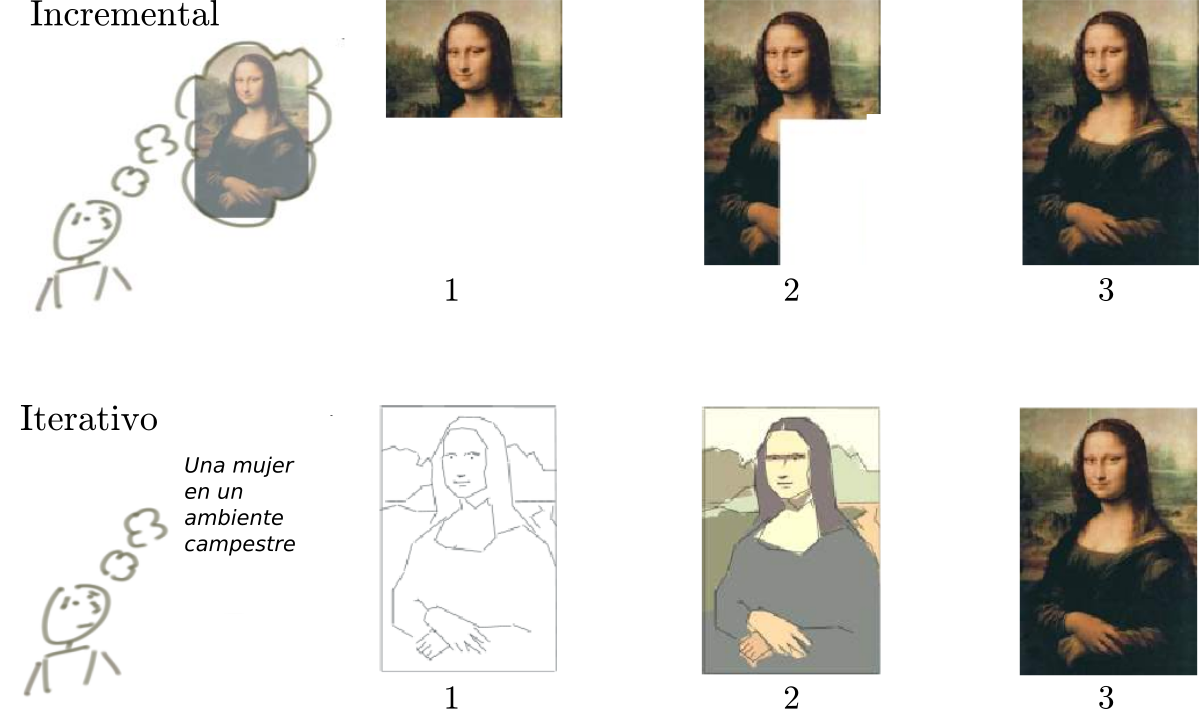
\includegraphics[width=12cm]{Img/CPD/mona.png}
\caption{\footnotesize{Diseño incremental vs iterativo.  }}
\label{fig: incremental}
\end{figure}


El concepto de iterativo se ha extendido con éxito a otras áreas como las metodologías \textit{\Gls{Agile}}  \citep{cockburn2002agile}.  
Por ejemplo, el marco de desarrollo \textit{\Gls{SCRUM}}\citep{Schwaber95scrumdevelopment} introduce el concepto de \textit{\Gls{sprint}}\footnote{Un Sprint, es un intervalo prefijado durante el cual se crea un incremento de producto ``Hecho o Terminado'' utilizable, potencialmente entregable} para referirse a la iteración.



\vskip


\subsubsection{Riesgo de la metodología en cascada frente a las iterativas}

{En este contexto, el riesgo se refiere a los factores que contribuyen al éxito o fracaso de un proyecto}. 
Todos los proyectos tienen algún riesgo, independientemente de su enfoque. En algunas situaciones, los factores inesperados que impactan positivamente el proyecto también son riesgos, pero se consideran  oportunidades.
Una regla que se aplica siempre es que \textbf{los riesgos negativos deben detectarse y mitigarse} \citep{layton2015scrum}. 

En la metodología en cascada existen una serie de factores negativos, propios de su estructura secuencial.
Un caso se puede analizar en la parte superior de la figura \ref{fig:water0} un modelo en cascada con las etapas \textit{definir, construir, testear y lanzar} para el desarrollo de un producto. Testear (probar) el producto justo antes del lanzamiento significa que si se presentan problemas en esa instancia se pone en riesgo todo el proyecto, la curva de riesgo incrementa notablemente justo al final de proyecto, en el lanzamiento. Por otro lado, en la parte inferior (ver figura \ref{fig:water0})  
se aprecia un modelo iterativo (Agile) con las mismas etapas definidas en todas las iteraciones. Si una decisión técnica, un requisito o incluso un producto completo no es factible, el equipo descubre esto en poco tiempo, por ende se cuenta con más tiempo para realizar correcciones. Si la corrección no es posible, de todas maneras el riesgo por el proyecto fallido es menor que con el enfoque en cascada \citep{Kukhnavets2016}.\vskip

\begin{figure}[ht]
\centering
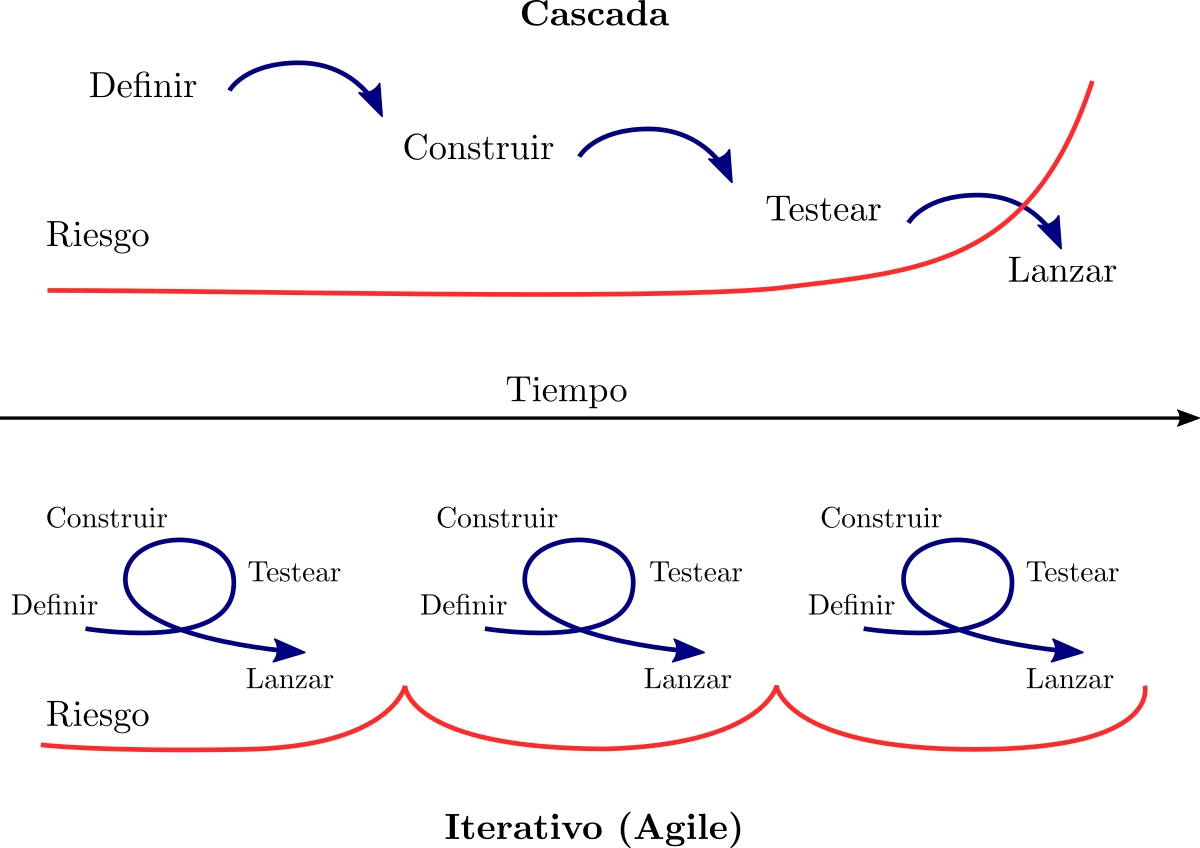
\includegraphics[width=13cm]{Img/CPD/cpd-water1.png}
\caption{\footnotesize{Riesgo de un proyecto en cascada vs iterativo (Agile).}}
\label{fig:water0}
\end{figure}
\vskip




Son evidentes las ventajas de la iteración y esto ha promovido que los nuevos productos se lancen a un ritmo creciente. Adicionalmente, tanto el hardware como el software evolucionaron para admitir la comunicación y el acceso multiusuario a los datos de diseño, la forma de acceso varía desde archivos compartidos hasta accesos compartidos mediante \textbf{Sistemas de Gestión de Bases de Datos} en inglés \textit{Data Base Management System} (\Gls{DBMS}) \citep{silberschatz2006fundamentos}. \vskip

Las aplicaciones CAD colaborativas se pueden identificar mediante una matriz (ver figura  \ref{fig:tablacad}) según su forma de uso en el tiempo y espacio \citep{Maher1997}. A continuación se analiza las diferentes configuraciones de la matriz.

\begin{enumerate}
    \item En el \textbf{mismo sitio y al mismo tiempo} es posible con una interfaz para un solo usuario, los diseñadores pueden compartir la misma computadora si necesitan colaborar.
    \item En el \textbf{mismo sitio pero en tiempos diferentes} es posible gracias a la gestión de datos técnicos, de manera que estén disponibles para la misma persona u otros miembros del equipo luego de que el diseño se completa.
    \item Al \textbf{mismo tiempo en sitios diferentes} se denomina 
    \textbf{CAD colaborativo} o bien \textbf{Co-Diseño}, diferentes diseñadores pueden ver y modificar el diseño en diferentes ubicaciones, viendo la misma imagen en la pantalla y comunicándose entre sí.
    \item En \textbf{sitios diferentes en tiempos diferentes} por consecuencia de la distribución de datos del diseño a través de una red (\textbf{CAD distribuido}), permitiendo a los actores acceder a los diseños independientemente de su ubicación y disponibilidad.
\end{enumerate}


La colaboración implica que el soporte informático (sistemas CAD) debe proporcionar flexibilidad en la comunicación de datos e ideas, considerando que el diseño colaborativo involucra muchos tipos de conocimiento de diferentes dominios. A continuación se analiza la forma en que los sistemas soportan estos paradigmas.


\vskip
\section{Sistemas CAD colaborativos}
\label{section:colabo}

\begin{figure}[ht]
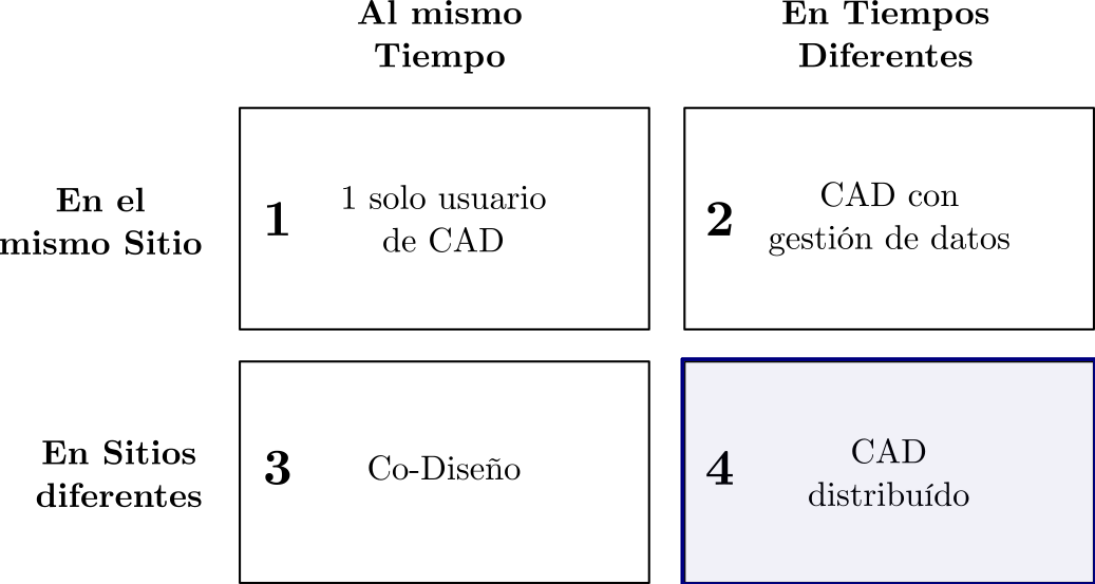
\includegraphics[width=10cm]{Img/CPD/cad-time.png}
\centering
\caption{\footnotesize{El uso del CAD en el espacio y tiempo}}
\label{fig:tablacad}
\end{figure}

El contenido compartido en los ambientes de \textbf{diseño colaborativo y distribuido} por lo general implica el uso de \textbf{modelos 3D} como medio de comunicación entre los participantes con el fin de visualizar ideas abstractas y se usan iterativamente durante todo el proceso de diseño \citep{Tek-JinNam2009}. Los participantes requieren diferentes vistas del diseño, pueden tener intereses diferentes respecto %desarrollo de 
a las soluciones y su representación asociada. De manera que, se necesitan múltiples niveles de abstracción en términos de soporte informático para gestionar la diversidad de conocimiento. %Además, para permitir la participación


\subsection{Soporte informático a la colaboración }
La colaboración se puede lograr mediante un \textbf{Espacio de Trabajo Compartido} en inglés \textit{\Gls{Shared Workspace}}  (ver figura \ref{fig:sistemashared}). 
Este proporciona una comunicación visual y funciona como un medio en el que un actor puede comprender el modelo/diseño de otro sin necesidad de tener el mismo vocabulario \citep{Maher2006}. 
Un espacio de trabajo compartido CAD se puede dividir en dos significados: El espacio de trabajo con el que los participantes humanos visualizan el diseño e interactúan y la representación compartida del problema de diseño que utiliza la propia computadora para la persistencia y la comunicación entre procesos. Por ende se consideran dos categorías de representaciones en el espacio de trabajo: \textbf{{Representación visual}} compartida y \textbf{Representación subyacente} compartida. Esto proviene de los requisitos de los sistemas multiusuario, en el que los usuarios puedan ver el trabajo de los demás. La parte visual es proporcionada por los modelos 3D y además con la posibilidad que el sistema mantenga una o más representaciones de la solución de diseño (versiones). Cualquier otro conocimiento de dominio relevante es proporcionado por el contenido subyacente, por ejemplo: referencias, documentación técnica, archivos extra para interactuar con otros sistemas, etc.

\begin{figure}[ht]
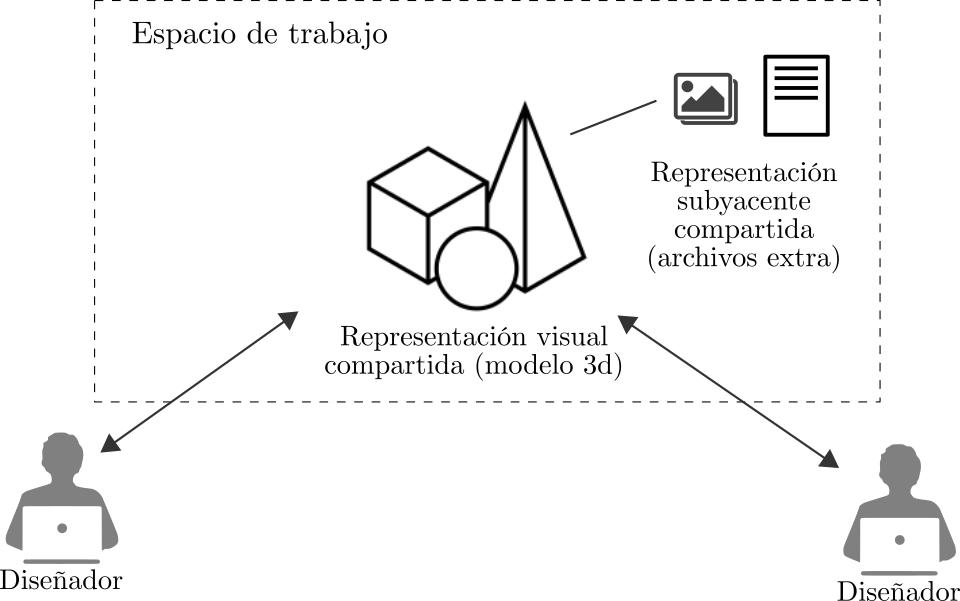
\includegraphics[width=10cm]{Img/CPD/cad-shared.png}
\centering
\caption{\footnotesize{Representaciones en un espacio de trabajo compartido.}}
\label{fig:sistemashared}
\end{figure}

Aparte de la implementación de un espacio compartido, resolver problemas como el modelado no es una tarea trivial para los sistemas y se necesita de una infraestructura y componentes con determinadas características. A continuación se explican los sistemas de modelado sólido.

\subsection{Sistemas de Modelado Sólido }

En la creación de un sistema de modelado de sólidos o ``modelador sólido'' se deben considerar las condiciones geométricas y topológicas explicadas en la sección \ref{ref:modelado-solido}. Mäntylä expone que la idea fundamental es separar el modelo geométrico de la aplicación y desarrollar técnicas de modelado que sean independientes de los objetos \citep{Mantyla:1988:ISM:60949}. Los pasos a dar se ilustran en la figura \ref{fig:sistema-solido} y pueden resumir de la siguiente manera:


\begin{itemize}
\item Inicialmente, 
los objetos son descritos por el usuario mediante un \textbf{lenguaje de descripción}, basados en los conceptos de modelado (poligonal, booleano, etc) aplicados al sistema. 
Se introducen utilizando \textit{scripting}, con lenguajes como OpenSCAD o \Gls{python}\footnote{\url{http://python.org}}, o bien mediante una \textbf{interfaz de usuario} para interactuar gráficamente. Un mismo sistema puede incluir varios lenguajes de descripción, atendiendo a diferentes usuarios y aplicaciones.

\item Una vez introducidos, los objetos son traducidos para crear la \textbf{representación interna} almacenada por el modelador. 
La relación entre el lenguaje de descripción y la representación interna no necesariamente debe de ser directa: las representaciones internas pueden emplear conceptos de modelado distintos a la descripción original. La transformación del lenguaje de descripción a la representación interna es necesaria para poder encontrar las respuestas a las preguntas geométricas. De hecho, para que un sistema de modelado sea eficiente, debe soportar múltiples representaciones internas de los objetos, por ejemplo con diferentes tecnologías para geometrías como \Gls{CGCAL}\footnote{\url{https://www.cgal.org/}} u \Gls{Open-Cascade}\footnote{\url{https://www.opencascade.com/content/latest-release}}. Por lo tanto, se deben incluir algoritmos de conversión que puedan modificar una representación en otra.

 \item Para comunicarse con otros sistemas de modelado  (importación/exportación) el modelador debe proveer interfaces de comunicación. 
 Estas interfaces son utilizadas para recibir o transmitir modelos hacia o desde otros sistemas de modelado. Necesariamente debe manejar información geométrica utilizando formatos existentes como por ejemplo \Gls{STEP} acrónimo de \textit{Standard for the Exchange of Product Data} \citep{Wilson1998} o \Gls{STL} acrónimo  de \textit{Stereolithography} \citep{grimm2004user}.

\item Finalmente, el modelador también debe incluir facilidades para almacenar las descripción de objetos y demás datos, en bases de datos permanentes. 
\end{itemize}

\begin{figure}[ht]
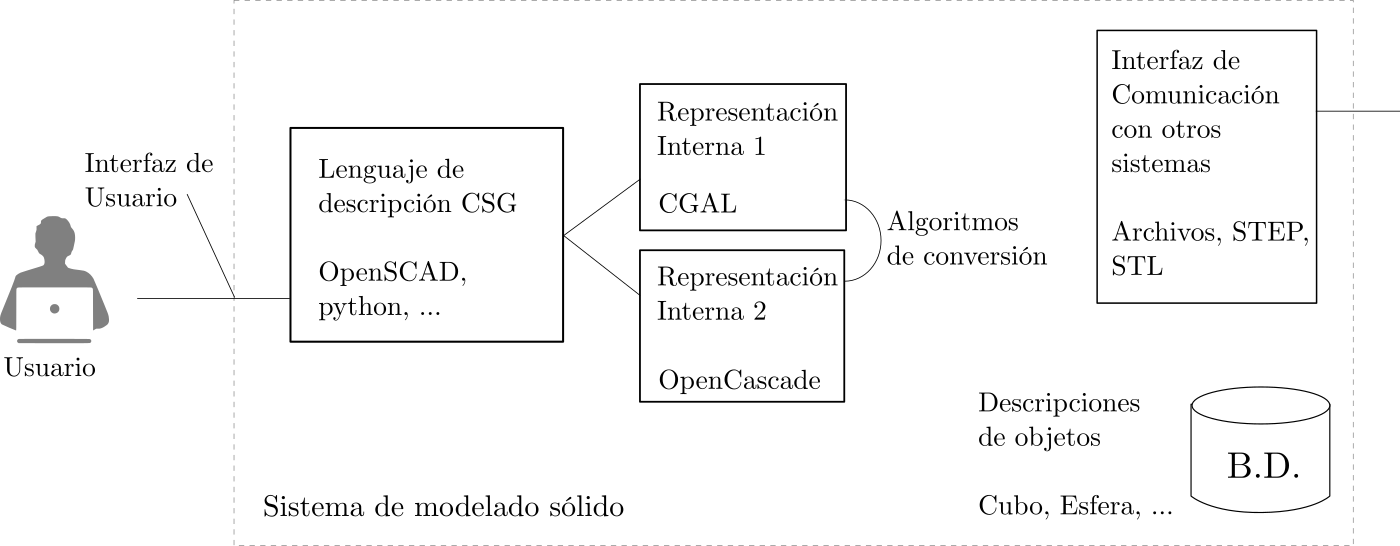
\includegraphics[width=14cm]{Img/GEO/sistema-solido.png}
\centering
\caption{ \footnotesize{Sistema de Modelado Sólido. 

%El usuario (izquierda) ingresa las descripciones de los objetos a través de la interfaz de usuario mediante un lenguaje de \textit{scripting} (OpenSCAD, python, etc). Luego, el lenguaje de descripción es traducido a la representación interna (GCAL, OpenCascade, etc) para encontrar las respuestas a las preguntas geométricas (centro). Si existen varias representaciones internas se utilizan los algoritmos de conversión. En la derecha se puede apreciar la Interfaz de Comunicación con otros sistemas y la Base de Datos permanente con las descripciones de los objetos (primitivas). \citep{Ramos2011}

}}
\label{fig:sistema-solido}
\end{figure}

En estos sistemas se pueden distinguir tres niveles de abstracción:

\begin{enumerate}
\item \textbf{Interfaz de usuario.} Mediante el lenguaje de descripción, el usuario utiliza las operaciones disponibles en cualquier aplicación CAD (crear, modificar, guardar, borrar y analizar diseños).
\item \textbf{Infraestructura matemática y algorítmica.}  Implementa las operaciones que proporciona el nivel anterior (por ejemplo, los algoritmos CSG para trabajar con objetos mediante operaciones booleanas).
\item \textbf{Primitivas.} A nivel de sistema, son operaciones aritméticas y lógicas que describen los objetos primitivos. Se encuentran disponibles de forma permanente en bases de datos para que puedan ser utilizadas por el nivel anterior.
\end{enumerate}

Dentro de la complejidad de un modelador es indispensable que los datos de los productos sean accesibles y carezcan de errores.
Para lograrlo se utilizan los sistemas de  \textbf{Gestión de Datos del Producto} en inglés \textit{Product Data Management} (\Gls{PDM}) \citep{Ruiz} los cuáles se explican a continuación.



\subsection{Gestión de Datos del Producto (PDM)}
\label{sec:pdm}
Max Ungerer define que \textquote{\textit{un sistema PDM es ``algo'' que maneja datos sobre productos}}. En el núcleo central de la información está la identificación del producto y se representa conceptualmente como un elemento o ítem dentro del sistema \citep{Ungerer2002}. \vskip


Para garantizar la colaboración distribuida, los PDM tradicionales tienen los mismos problemas que las aplicaciones de escritorio:

\begin{enumerate}
    \item {Es difícil proporcionar acceso a los usuarios desde diferentes ubicaciones}, especialmente aquellos que se encuentran en diferentes redes. En cada implementación del PDM, las configuraciones de red deben ser homogéneas. 
    \item {Las aplicaciones cliente\footnote{El cliente es una aplicación informática  que consume un servicio remoto} son dependientes de la plataforma}, todos los usuarios deben usar la misma plataforma informática o bien se debe proporcionar una aplicación específica para cada plataforma de usuario. Actualmente, es casi imposible este mandato por la diversidad de sistemas y dispositivos. 
    \item {Las tareas de ampliación y actualización no son sencillas}, cuando se requieren nuevas funciones, los usuarios deben volver a instalar o actualizar la aplicación completamente. 
\end{enumerate}

En consecuencia, es lógico utilizar un \textbf{PDM basado en la web} en inglés \textit{Web based Product Data Management} (\Gls{WPDM}) \citep{Huang2004} porque pueden ofrecer soluciones centradas en la lógica de negocio de las empresas y proporcionar una comunicación global sin mucho esfuerzo, brindando funciones independientes de las redes y la plataforma. Esto se traduce en una reducción del costo general para la implementación. Un WPDM eficiente requiere:
\begin{itemize}
    \item Ser totalmente escalable para proporcionar flexibilidad, porque cada organización tiene diferentes prioridades y diferentes flujos de trabajo.
   \item Ser sencillo de usar por todos los participantes.
    \item Tener una arquitectura abierta para que se permite añadir, modernizar y cambiar sus componentes sin depender de un proveedor.
    \item Estar disponible en una amplia variedad de plataformas y proveer funciones en redes heterogéneas.
\end{itemize}

La mayoría de los sistemas WPDM que se han implementado con éxito hacen uso de \textbf{Servicios Web} en inglés  \textit{\Gls{Web Services}} \citep{richardson2008restful}.


\subsection{Intercambio de datos CAD}
En el pasado, el proceso de intercambio de datos estaba relacionado con los planos y los documentos técnicos, actualmente se requieren archivos digitales  compartidos entre múltiples aplicaciones.
Los esfuerzos hacia la integración del CAD generaron 
el desarrollo de varios formatos estándares para el \textbf{Intercambio de Datos de CAD} en inglés \textit{CAD Data Exchange} \citep{Randjelovic2007}, así como muchos ``no estándares". Los formatos han variado desde archivos para datos de dibujo técnico como DXF\footnote{\url{https://es.wikipedia.org/wiki/DXF}} hasta representaciones de modelos 3D como STEP \citep{Wilson1998}. 

En lo ámbitos de fabricación digital el \textit{CAD Data Exchange} es la norma, a pesar de que cada sistema tiene su propio formatos de datos. Así, la misma  información puede ser ingresada varias veces en diferente sistemas, provocando redundancia.   
Además, el uso de modelos 3D de geometría compleja puede provocar errores en los datos de diseño, con  representaciones incorrectas y falta de entendimiento entre los actores. Respecto a esta problemática, desde el año 1999 el Instituto Nacional de Estándares de EE.UU.  (NIST)\footnote{\url{https://www.nist.gov/}} estima que la incompatibilidad de datos se traduce en costos que alcanzan los 90 millones de dólares por año  \citep{Tassey1999}. \vskip

En conclusión, el \textit{CAD Data Exchange} es fundamental en el contexto actual del modelado geométrico, ya que es el mecanismo principal para lograr interoperabilidad la entre las diferentes plataformas.

\subsubsection{Data Exchange Geométrico}


El enfoque establecido para el intercambio de datos se denomina \textbf{Data Exchange de la geometría} o \textbf{\Gls{DE} geométrico} \citep{Spitz:2004:IFG:1217875.1217904}, en este la representación del objeto se transfiere de un sistema origen a un sistema de destino. En las aplicaciones comerciales se implementan a través de los \textbf{formatos neutrales} que pueden ser generados y leídos en la mayoría de los sistema CAD. Algunos ejemplos de ellos son STEP y STL, acrónimo  de \textit{STereoLithography} \citep{grimm2004user}. 
\vskip
STEP interpreta un producto como uno o varios documentos. Utiliza \textbf{grupos de conceptos} para organizar los elementos de manera lógica y así generar una estructura clara y comprensible para todas las plataformas. Su estructura depende de la dirección que tome el sistema PDM, sus protocolos de aplicación y su alcance. \vskip 

Por su parte, los archivos STL describen la geometría de un objeto 3D mediante triángulos, sin considerar la representación de color, textura u otros atributos. Se pueden especificar tanto en \Gls{ASCII} como en binario y se caracterizan por ser ampliamente utilizados para fabricación digital. 
\vskip 


El uso del DE geométrico con formatos neutrales o nativos es bastante confiable, aunque muchas veces es posible obtener resultados de modelos no sólidos debido a la perdida de información de sus estructuras.
No obstante, su principal inconveniente no es la inconsistencia geométrica, sino el hecho de que no es compatible con el paradigma de diseño más común de la actualidad: el diseño \textbf{basado en características} en inglés \textit{Feature Based} (\Gls{FB}), también llamado \textbf{diseño paramétrico} o \textbf{diseño basado en la historia} como se explica en la sección \ref{cadparam}.
Por esa razón es imposible realizar modificaciones de los modelos en el lado del sistema destino. Esta situación se puede ver ilustrada en el ejemplo de la figura \ref{fig:de0}. El usuario en el sistema origen (izquierda) puede visualizar y modificar el modelo para compartir con el sistema destino mediante un archivo en formato STEP que incluye los datos geométricos. Por otra parte el usuario en el sistema destino (derecha) puede visualizar el modelo pero no modificarlo, puesto que solamente tiene acceso a los datos geométricos, pero no a los parámetros necesarios para alterar la representación. 

\begin{figure}[ht]
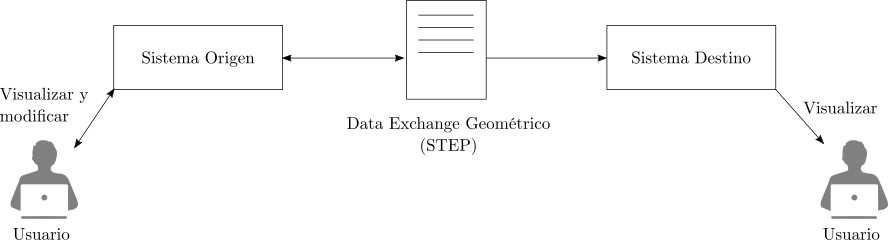
\includegraphics[width=14cm]{Img/WEB/de0.png}
\centering
\caption{\footnotesize{Esquema de Data Exchange Geométrico. 
}}
\label{fig:de0}
\end{figure}

De esta limitación surge el  \textbf{Intercambio de Datos Basado en Características} en inglés \textit{Feature Based Data Exchange} (\Gls{FBDE}) \citep{Spitz:2004:IFG:1217875.1217904}.

\subsubsection{Data Exchange basado en características (FBDE)}
\label{FBDE}

En el FBDE, dado un grafo o estructura  basada en el historial paramétrico de un modelo (características) en un sistema origen, el objetivo es construir un grafo en un sistema destino con una geometría similar, conservando al mismo tiempo la mayor información paramétrica posible. En muchos casos, la geometría puede no ser idéntica debido a diferentes políticas de tolerancia entre los sistemas CAD. Siempre que la aproximación esté controlada es totalmente aceptable en la práctica. \vskip
El FBDE conserva la inteligencia del diseño, permitiendo que se realicen modificaciones en el lado del sistema destino (ver figura  \ref{fig:de1}). El usuario en el sistema origen (izquierda) puede visualizar y modificar el modelo. La compartición del modelo se realiza mediante un formato o tipo de fichero que contiene los datos geométricos y también expone las características del modelo mediante los parámetros. En el sistema destino (derecha) se puede visualizar y manipular el modelo debido a que posee los datos geométricos y paramétricos para modificar la representación. 

\begin{figure}[ht]
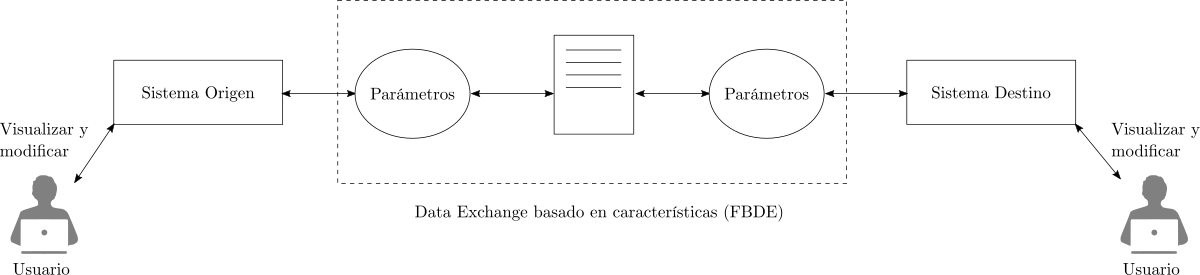
\includegraphics[width=16cm]{Img/WEB/de1.png}
\centering
\caption{\footnotesize{Esquema de Data Exchange basado en características (FBDE). }}
\label{fig:de1}
\end{figure}

Adicionalmente, el sistema debe contar con mecanismos para evitar o reparar problemas de inconsistencias geométricas en los archivos de intercambio.\vskip
El modelo se suele representar como un árbol o lista de operaciones, comúnmente llamado \textbf{árbol de historia}. Las operaciones crean una nueva geometría o modifican una existente. Esta estructura se puede considerar una extensión de la geometría constructiva de sólidos (CSG) explicada en la sección \ref{mod:booleano}. El punto principal de este paradigma es que las operaciones son siempre de naturaleza paramétrica. 

En la figura \ref{fig:de2} se ilustra un ejemplo con las diferentes versiones de un modelo mecánico (derecha) y su representación como árbol de historia (FBDE) (izquierda). Las versiones se producen a partir de las operaciones o modificaciones de los parámetros, desde un \textbf{modelo original} hasta un \textbf{modelo objetivo}. En cada nivel del árbol se pueden ver las operaciones realizadas.  Partiendo del modelo original, para obtener la \textit{Versión \#1} se modifica el parámetro \textit{cilindros\_B = 0} a \textit{cilindros\_B = 8} de manera que se agregan 8 cilindros. Esta operación genera una separación entre la pieza y los cilindros, produciendo un objeto ``no sólido''. La \textit{Versión \#2} soluciona este problema, convirtiendo al objeto nuevamente en sólido con la modificación de la variable \textit{cilindros\_A = 8} y su correspondiente incorporación de 8 cilindros de base. Finalmente a la \textit{Versión \#2} se aplica un operador booleano de  intersección entre el modelo y un cilindro, generando un orificio en el modelo objetivo 
\citep{Kwon2015}.

\begin{figure}[ht]
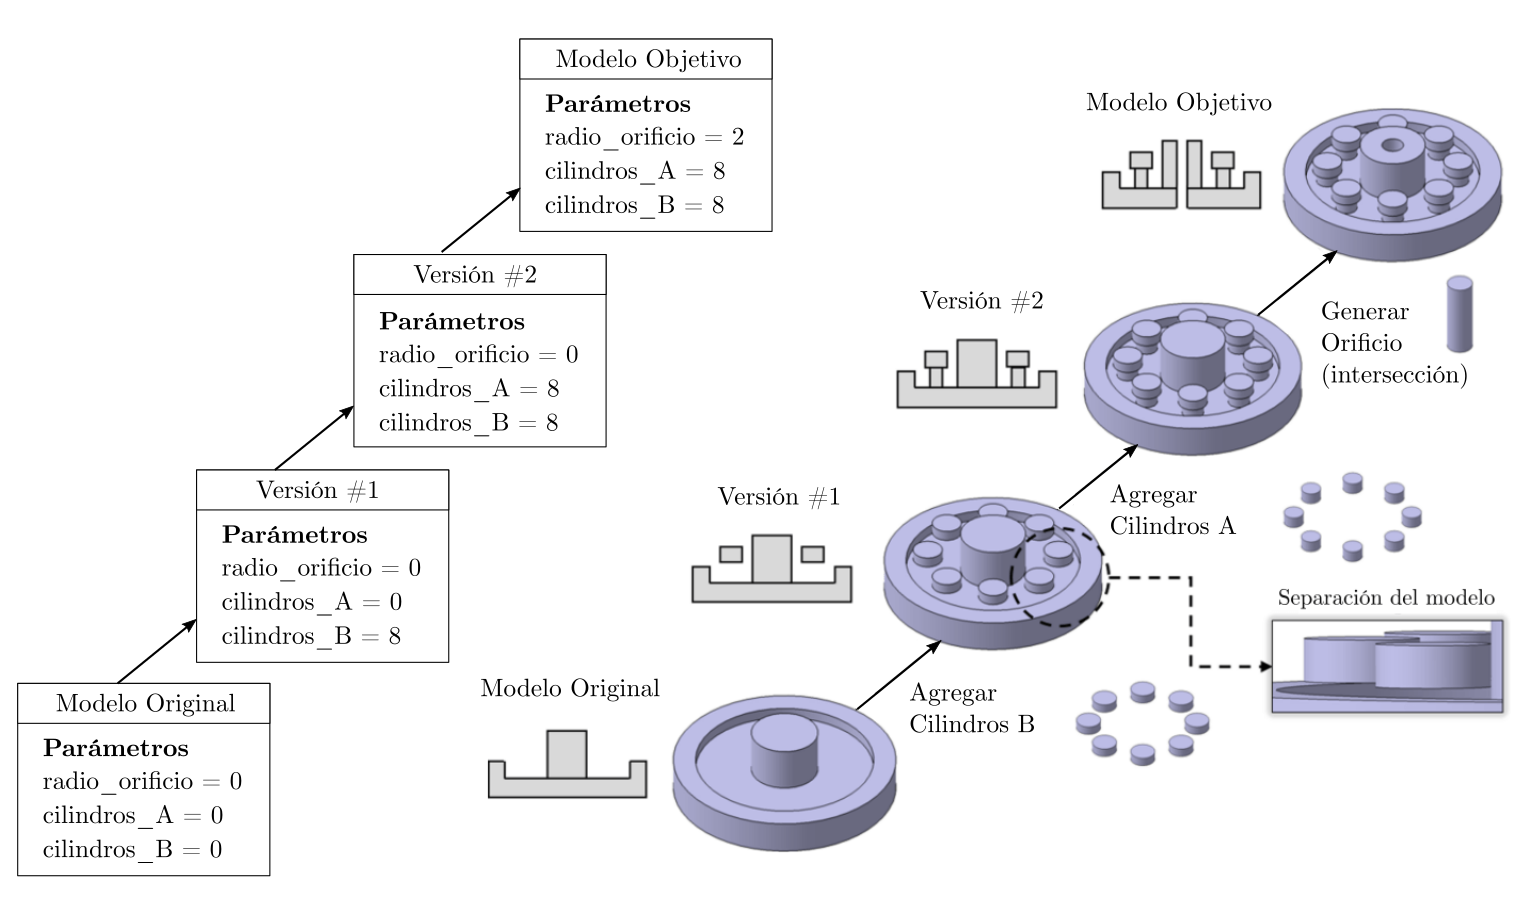
\includegraphics[width=16cm]{Img/WEB/de-fin.png}
\centering
\caption{\footnotesize{ Modelo mecánico y su representación como árbol de historia (FBDE). }}
\label{fig:de2}
\end{figure}



Por lo anteriormente expuesto, es deseable un sistema de \textbf{CAD distribuido} que permita el \textbf{co-diseño} de productos orientados a la \textbf{fabricación digital}, este debe tener capacidades para la  gestión de datos de productos basados en la web \textbf{(WPDM)} y soporte al intercambio de datos basados en características \textbf{(FBDE)}.

Para que el desarrollo del sistema esté en sintonía con los principios colaborativos planteados, se pueden utilizar metodologías o enfoques orientados a la experiencia de usuario (UX) como \textit{Lean UX}.  

%\clearpage
\section{Lean UX}
\label{section:pmv}
Los equipos de desarrollo de software son un ejemplo de eficiencia en la colaboración, utilizan técnicas de desarrollo ágil \citep{cockburn2002agile}, reduciendo drásticamente el tiempo que requiere modificar una aplicación, realizan cambios en el código y 
lo llevan a producción\footnote{Producción es la instancia del software cuando se encuentra a disposición de los usuarios finales.} a una velocidad similar a la de guardar un archivo en un ordenador. Además,  utilizan mecanismos para iterar incorporando lo que han aprendido y tal vez, sin advertirlo, aumentan las expectativas de los usuarios.  \Gls{GitHub}\footnote{\url{https://github.com/}} es un caso de éxito como plataforma de trabajo colaborativo, convirtiéndose en la herramienta de gestión de código más utilizada en la actualidad \citep{GitHub2018}.
En este nuevo contexto, las prácticas de analizar todo el proyecto al inicio quedaron obsoletas. \vskip
\textit{Lean User Experience} (Lean UX) \citep{Gothelf2013} 
es una metodología que utiliza las herramientas disponibles y las combina de forma diferente para adecuarlas a esta nueva realidad. Jeff Gothelf y Josh Seiden la describen como \textquote{\textit{una nueva etapa evolutiva en el diseño de productos}}. 
Se considera profundamente colaborativa y multidisciplinaria, en gran medida porque permite implementar técnicas para construir una comprensión compartida del proyecto, logra un ambiente propicio para el \textit{\gls{feedback}} con los usuarios finales, replantea las conversaciones de diseño en términos objetivos y cambia la forma en que se comunica el diseño del producto: en lugar de hablar de funciones y documentos, se habla de lo que efectivamente funciona y de lo que no.


\vspace{5mm}

Los \textbf{3 pilares principales de Lean UX} son:
\begin{enumerate}
    \item \textbf{Design Thinking o Pensamiento de Diseño} \vskip
    
    El \textit{Design Thinking} \citep{Brown2009} logra obtener soluciones involucrando a los usuarios para convertirlos en actores activos en todo el proceso de la construcción del producto. 
    Es una manera de trabajar que alienta la colaboración del  equipo, independientemente del rol que cada actor desempeñe. Centra su eficacia en entender y dar solución a las necesidades reales de los usuarios.

    \item \textbf{Metodologías de desarrollo ágil de software}.\vskip
    Los desarrolladores de software las han usado durante mucho tiempo.
    No obstante, estas  constituyen un reto para los diseñadores. \textit{Lean UX} aplica los 4 principios básicos del desarrollo ágil al diseño de productos \citep{Gothelf2013} :
        
        \begin{enumerate}
        \item
        \textbf{Los individuos y las interacciones son más importantes que los procesos y las herramientas}: 
        Para generar rápido las mejores soluciones, se debe implicar a todo el equipo. 
        La comunicación fluida  debe primar por encima de las restricciones propias de las herramientas.
        \item
        \textbf{El software funcional es más importante que la documentación exhaustiva}: 
        Un software que funcione es más importante que preocuparse por una documentación exhaustiva. De esta manera, se puede encontrar de antemano la solución que mejor se adapte a las necesidades.
        \item
        \textbf{La colaboración con los clientes es más importante que la negociación de contratos con ellos}: 
        Si el equipo colabora con los usuarios/clientes, hay un entendimiento común sobre los problemas y las posibles soluciones. Cualquier decisión se debe tomar por consenso, esto se traduce en iteraciones más rápidas y una verdadera implicación de todos los actores con la ventaja de trabajar siempre con soluciones validadas. 
        \item
        \textbf{La respuesta a los cambios es más importante que la planificación}: 
        Se asume que el equipo no encontrará la solución la primera vez, por lo que el objetivo consiste en averiguar en que se ha fallado. Luego se pueden ajustar las propuestas y volver a probarlas iterativamente. 
        \end{enumerate}

\item \textbf{Método Lean Startup}\vskip 

Los proyectos han estado enmarcados, tradicionalmente, por los requerimientos y las entregas. A los equipos se les suministraban requerimientos para que produjeran entregas.
No se inicia a partir de requerimientos, sino de  suposiciones. A partir de ellas, se crean y prueban \textbf{hipótesis} o \textquote{una manera de expresar las suposiciones que se tienen del proyecto de una forma comprobable} \citep{Gothelf2013}. 

\textit{Lean Startup} \citep{ries2012metodo} utiliza un ciclo de \textit{feedback} denominado \textbf{``construir-medir-aprender''} que minimiza el riesgo de los proyectos y  consigue que el equipo pueda desarrollar software y aprenda de él en muy poco tiempo (ver figura \ref{fig:ciclolean}). Consiste en poner en marcha (construir) las ideas que se suponen van a tener éxito, medir y recabar los datos para confirmar o desmentir las hipótesis que se plantearon al principio y aprender del fracaso o el éxito resultante. En el centro de la figura se aprecia la interacción entre las ideas, el producto construido (\Gls{PMV}) y los datos recabados \citep{Borodin2018}.

\begin{figure}[h]
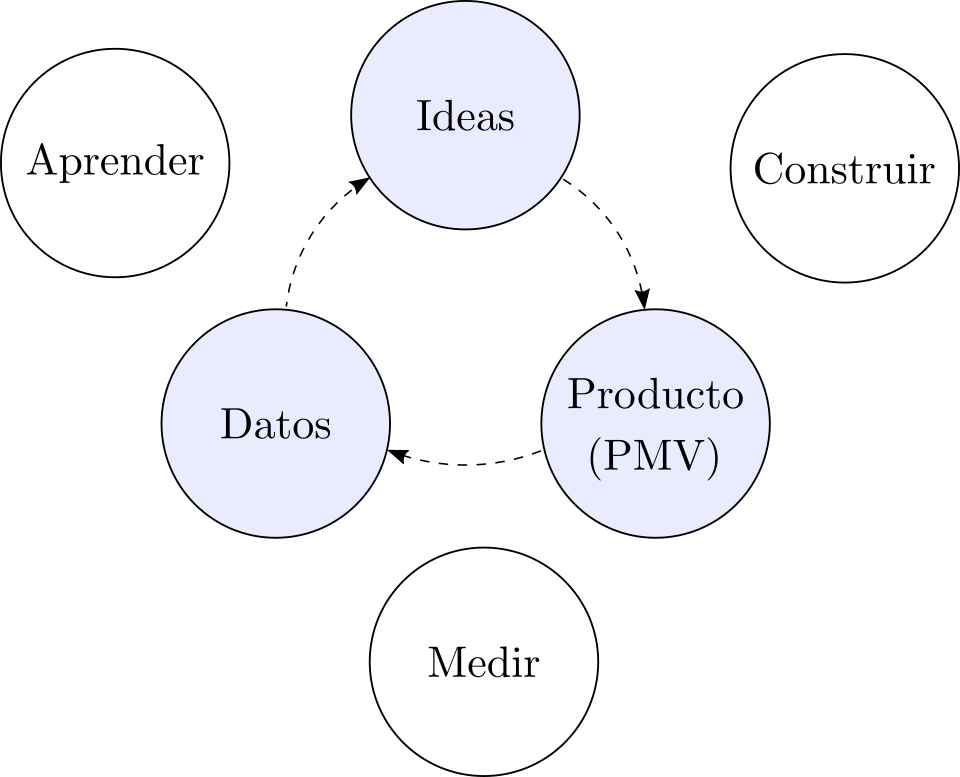
\includegraphics[width=7cm]{Img/Desarrollo/lean1.png}
\centering
\caption{\footnotesize{Ciclo Construir-Medir-Aprender.}}
\label{fig:ciclolean}
\end{figure}


De esta manera, los equipos pueden desarrollar de inmediato los denominados \textbf{Productos Mínimos Viables} (PMV) en inglés \textit{Minimum Viable Products} (MVP) \citep{olsen2015lean}. El ciclo se desarrolla de la siguiente manera:


    \begin{itemize}
    \item En primer lugar, se construye un PMV, es decir, \textbf{el desarrollo más pequeño que pueda construirse para probar cada hipótesis}. Se debe tener en cuenta que tanto el PMV inicial como las siguientes iteraciones deben tener valor por sí mismas. Es decir, se debe obtener un \textit{feedback} del usuario final. Para esto, el producto debe tener el mismo tratamiento utilizado en el diseño iterativo. Para un mejor entendimiento de este punto, se puede analizar la figura \ref{fig: incremental} explicada en la sección \ref{iterativo}.
    

    \item El siguiente paso es entregar el PMV a los usuarios y realizar experimentos que puedan ser medidos para obtener datos.
    \item Después, se utiliza lo aprendido con ellos para evaluar las hipótesis y hacer las modificaciones pertinentes.
    \item Y finalmente se itera, se comienza todo el proceso nuevamente. 
    \end{itemize} 


\end{enumerate}

%\clearpage
\subsubsection{Proceso Lean UX}
El objetivo final es trasladar todos los valores heredados de los 3 pilares al trabajo de experiencia de usuario mediante un conjunto de pasos definidos, métodos y herramientas que se analizan a continuación.

\begin{figure}[h]
    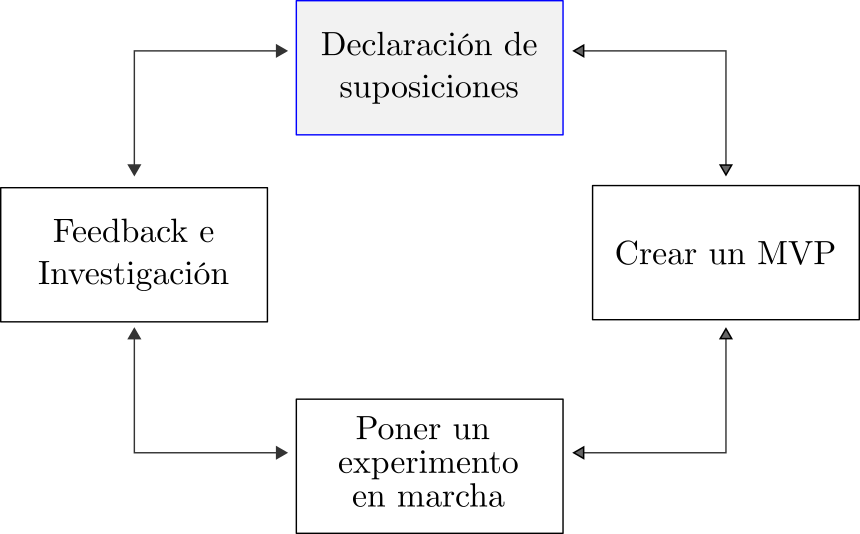
\includegraphics[width=9cm]{Img/Desarrollo/desarrollo1.png}
    \centering
    \caption{\footnotesize{Proceso Lean UX. }}
    \label{fig:leanux1}
\end{figure}
    
\subsubsection{Declaración de suposiciones}
Antes de cualquier declaración, se realiza una exploración  recurriendo a técnicas de investigación en inglés \textit{\gls{research}} \citep{sharon2016validating} sobre los usuarios y sus necesidades. Estas declaraciones se componen de los siguientes elementos:


\begin{itemize}
    \item \textbf{Suposiciones}: una declaración de alto nivel que se considera cierta. 
    El primer paso en \textit{Lean UX} es declarar las suposiciones (ver figura \ref{fig:leanux1}), este ejercicio se realiza en equipo,  asegurándose de que todas las disciplinas estén representadas. Con toda la información recolectada se continúa con la declaración del problema.
    
    \textbf{Método: Declaración de problema}\vskip
    \label{sec:dec-problema}
    Permite centrar correctamente el trabajo de todo el equipo y  define las restricciones y límites necesarios para que no se pierda  de vista el objetivo. Se puede utilizar la siguiente plantilla:
    \textquote{[El servicio/producto] debe cumplir con [estos objetivos]. Sin embargo, se ha observado que no se están alcanzando [estos objetivos], lo que está causando [este efecto adverso] para los usuarios. ¿Cómo se podría mejorar el  [servicio/producto] de modo que los usuarios consigan mejorar sus resultado según [estos criterios cuantificables o cualificables]?}\vskip
    
    Generalmente las declaraciones está repletas de suposiciones, para extraerlas se utiliza una lista u \textbf{hoja de suposiciones}.

En base a las siguientes preguntas, se recopilan las declaraciones que reflejen lo que el equipo de desarrollo considere cierto respecto a la solución o producto. 
\textbf{¿Quiénes son los usuarios del producto?  
¿Cómo encaja en su trabajo? 
¿Qué problemas soluciona? 
¿Cuáles son sus funciones más importantes? ¿Qué aspecto debe tener y cómo debe comportarse?}

Si existen diferencias en un punto, lo mejor es reflejar esto de inmediato para facilitar la discusión entre los miembros del equipo de desarrollo. Una vez obtenida la lista de suposiciones priorizada, es necesario probarlas. 
    
    \item \textbf{Hipótesis}: descripciones más detalladas de las suposiciones, dirigidas a áreas específicas del producto o flujos de trabajo 
    con las que se puede experimentar.
Es decir, se transforman las suposiciones
a un formato más sencillo de probar.
Sin embargo, las hipótesis suelen ser demasiado extensas para que, con una única prueba, se pueda determinarse su validez. Contiene demasiadas partes, es decir, demasiadas ``sub-hipótesis''. Para 
registrar estas partes más pequeñas y específicas se utiliza la siguiente plantilla: \vskip

\textquote{Se considera que [haciendo esto, desarrollando esta función, creando esta experiencia de usuario] para [estas  personas] se conseguirá [este resultado]. 
Se sabrá si esto es correcto cuando se obtenga [esta medida cuantitativa, o este conocimiento cualitativo]}.\vskip 

El primer campo se completa con la función o mejora para el producto. El segundo describe exactamente qué usuarios objetivo se beneficiarán de la función. El último, especifica los beneficios que esos usuarios obtendrán de ella. La frase final lo une todo. Esta frase determina si la hipótesis es cierta o no.

    \item \textbf{Resultados}: los datos de entrada, proveniente de la experiencia de los usuarios, que ayudan a validar o invalidar las hipótesis. Pueden ser cuantitativos o  cualitativos.
    En principio se encuentran con resultados de alto nivel o generales. Se debe considerar cómo dividir esos resultados en componentes más pequeños, 
    específicos y cercanos a la realidad del proyecto.
    ¿Qué funciones en la UI podrían generar un mayor uso? ¿Un visor 3D totalmente funcional o simplemente compartiendo imágenes? Mediante estas preguntas, se enuncian resultados que se acercan a las necesidades reales del proyecto. Ejemplo: \textbf{Dar soporte a la visualización de modelos 3D en la web}.
    
    \item \textbf{Personas}: son modelos o arquetipos \citep{Gothelf2013} de los potenciales usuarios  para las que se considera estar resolviendo el problema.
    Detallan quién utilizará el producto y por qué lo hará. Se inicia con esquema muy sencillo, en cuya creación participa todo el equipo. A medida que se avanza en la investigación se pueden realizar ajustes.\vskip
    
    \item \textbf{Funciones o funcionalidades}: son las técnicas, las funciones, los productos y los servicios a desarrollar para conseguir los resultados. Normalmente, en este punto todos los miembros del equipo tienen su propia opinión, ya que, después de todo, las funciones son lo más concreto con lo que trabajan y les resulta más sencillo expresar sus ideas en términos de funciones. Sin embargo, un error común es hacer que el proceso de diseño parta de las funciones.
    
    

    Con todo el material obtenido se organizan las sub-hipótesis que deben probarse en una \textbf{tabla de sub-hipótesis}. La tabla se organiza con el siguiente formato: Función / Persona / Resultado.

\end{itemize}

\subsubsection{Diseño Colaborativo}

\label{dis-colabo}
 Con la \textbf{tabla de sub-hipótesis} como guía se reúne a diseñadores y no diseñadores (programadores, administradores de proyectos) 
 para crear los conceptos del producto 
 , y un entendimiento común sobre el problema y las soluciones de diseño. 
 Asimismo, permite decidir qué  elementos de la interfaz gráfica implementan mejor las funciones recogidas en las hipótesis.
 A continuación se describen dos herramientas utilizadas para el diseño de interfaces.
 
 \begin{itemize}
     \item \textbf{Estudio de diseño}: 
    \textquote{\textit{Un equipo interdisciplinario se reúne en una sesión de trabajo o \textbf{Estudio de Diseño} (a veces también llamado Charrette de diseño)}}\citep{Gothelf2013}. Permite explorar y analizar qué elementos de la interfaz gráfica pueden implementar mejor las funciones recogidas en las hipótesis.
    La documentación de salida de las sesiones constan normalmente de \textbf{esquemas de baja fidelidad} en inglés \textit{\gls{Sketch}} (ver figura \ref{salida}). Es esencial que la documentación no sea muy elaborada para que el trabajo continúe siendo maleable. De esta manera, el equipo puede cambiar de dirección con facilidad si las pruebas demuestran que el enfoque adoptado no es el correcto.
    \item \textbf{Guía de estilo}: 
    \label{style}
    En base a la documentación resultante del estudio de diseño se desarrolla la \textbf{guía de estilo}, una biblioteca de patrones aceptada por todo el equipo, para codificar los elementos gráficos e interactivos de la interfaz de usuario. También sirve para recopilar los componentes web en inglés \textit{\Gls{Web Components}}\footnote{\url{https://www.webcomponents.org/introduction}} del producto, todo lo que forme parte de la experiencia de usuario (UX) aparece en la guía de estilo. No solo se define el aspecto y el comportamiento, sino que también se proporciona la codificación de los componentes y las hojas de estilo en inglés \textit{Cascading Style Sheet} (\gls{CSS})\footnote{\url{https://www.w3.org/Style/CSS/}}. De esta manera, al modificar la guía de estilo también se modifica el producto. 
    
    \end{itemize}
 

\subsubsection{PMV y experimentos}

\label{pmv-cocada}
Con la lista de sub-hipótesis  se crean los PMV, explicado en la sección \ref{section:pmv}. Se utilizan para hacer experimentos y determinar qué ideas sobre el producto son válidas y cuáles deben descartarse.
Una de las maneras más efectivas de crear los PMV es mediante un prototipo de la experiencia. \textquote{\textit{Un prototipo es una aproximación de la experiencia de usuario que permite simular cómo será el uso de un producto o servicio}} \citep{Gothelf2013}. Es recomendable probar el PMV en primera instancia con todo el equipo de desarrollo, y luego con otras personas. Cuánto más se exponga a las miradas ajenas, más conocimiento se tendrá para validarlo. El siguiente paso es la experimentación de los usuarios finales. La idea es dejar que lo utilicen libremente, 
así se puede obtener todo el \textit{feedback}
posible sobre la experiencia.\vskip

\subsubsection{Feedback}
Hasta ahora, todo el trabajo está basado en las suposiciones; a partir de este punto se comienza con el proceso de validación. 
Un error común es realizar este proceso pocas veces, normalmente al principio del proyecto o al final.
La investigación es continua, lo que significa que se realizan en cada \textit{sprint} o iteración del producto.



Como consecuencia de usar este enfoque se obtiene: un equipo que trabaja de forma colaborativa, iterativamente, reduciendo al mínimo los documentos entregables, enfocándose en el software funcional y en el \textit{feedback} con el usuario final.


\section{Antecedentes}
\subsubsection{Speckle}
\Gls{Speckle} \citep{TheBartlett2015} comenzó como una investigación de diseño colaborativo para arquitectura en \textit{The Bartlett School of Architecture} (UCL)\footnote{\url{https://www.ucl.ac.uk/bartlett/architecture/}}.
El proyecto permite que los usuarios puedan compartir diseños paramétricos en la web. En la figura \ref{fig:spekle} se puede ver un modelo paramétrico en la plataforma web Speckle, a la izquierda se pueden apreciar los parámetros del modelo \citep{Dimitrie2017}. \\
El proyecto consta de:
\begin{itemize}
    \item Un plugin denominado \textit{Speckle Streams}\footnote{\url{https://www.food4rhino.com/app/speckle-streams}}  para el ecosistema del software  Rhino\footnote{\url{https://www.rhino3d.com/}}, este permite establecer los parámetros de los modelos y exportarlos a archivos en un formato específico.
    \item Una plataforma web que permite subir los archivos generados por el plugin para visualizar modelos 3D paramétricos, generar versiones modificadas, registrar un historial de los cambios y colaborar con otros usuarios.
\end{itemize}

\begin{figure}[h]
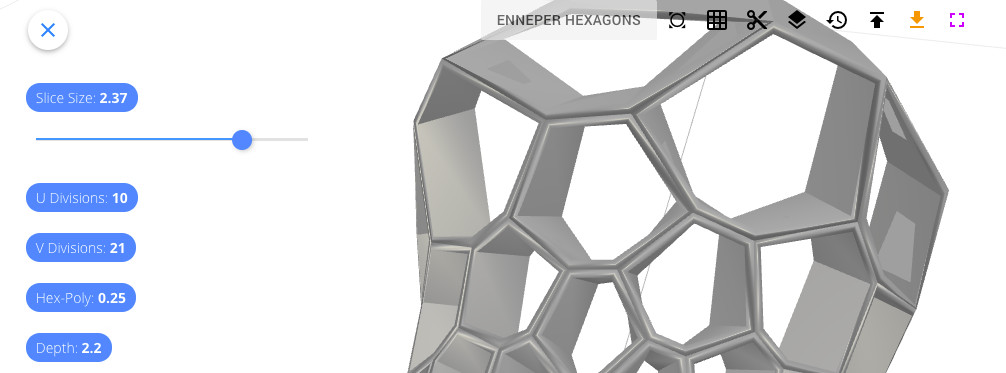
\includegraphics[width=14cm]{Img/Desarrollo/speckle.jpg}
\centering
\caption{\footnotesize{Interfaz web de Speckle.}}
\label{fig:spekle}
\end{figure}

Lo destacado de esta plataforma es la manera intuitiva de visualizar y modificar los modelos mediante su interfaz con componentes visuales como campos de texto, deslizadores, etc. \textbf{Speckle.Works}\footnote{\url{https://github.com/speckleworks}} es el repositorio FLOSS del proyecto que permite contribuciones de la comunidad. Actualmente se desarrollan diversas herramientas para la integración con otros softwares como Blender. 


\subsubsection{Modelo.io}
 Es una plataforma web creada por Qi Su y Tian Deng  \citep{Modelo.io2018} orientada a profesionales que utilizan Rhino y SketchUp\footnote{\url{https://www.sketchup.com/es}}. La característica de esta herramienta es que permite una colaboración efectiva entre los miembros de un equipo para perfeccionar los diseños y presentarlos de forma interactiva.

Los usuarios pueden explorar los modelos 3D, realizar comentarios, capturas de pantalla, anotaciones sobre los modelos, almacenar archivos extras asociados a los proyectos y otras características avanzadas como crear presentaciones 3D interactivas para los clientes. 
Se utiliza principalmente en   proyectos de arquitectura y diseño de interiores (ver figura \ref{fig:modelo.io}). En la interfaz web de \Gls{Modelo.io}, a la derecha se puede apreciar la interacción entre los usuarios \citep{Anthony2016} en un proyecto de arquitectura.

\begin{figure}[h]
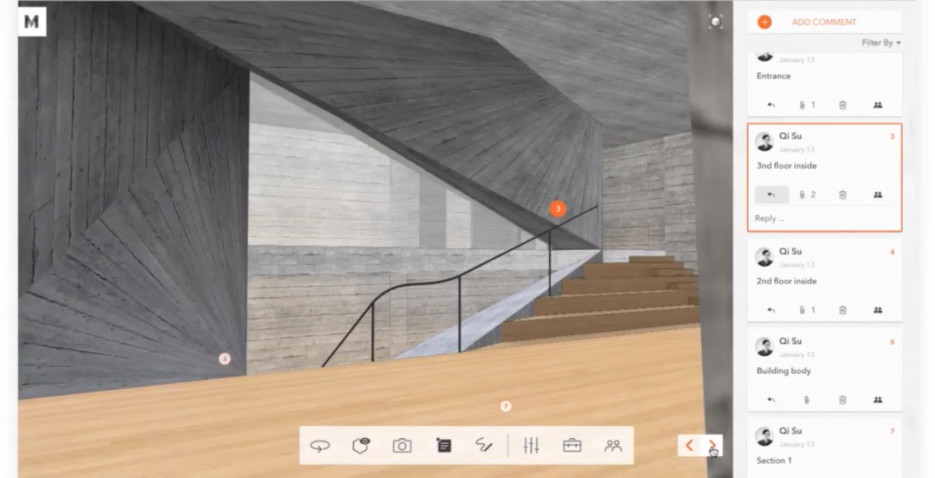
\includegraphics[width=14cm]{Img/Desarrollo/modeloio.jpg}
\centering
\caption{\footnotesize{Interfaz web de Modelo.io.}}
\label{fig:modelo.io}
\end{figure}




%\subsubsection{Problemas encontrados}
%En este trabajo se han presentado herramientas que soportan características relacionadas con el modelado especificado en algoritmos y la colaboración mediante modelos 3D. Los entornos analizados que permiten el modelado en la web son: OpenJSCAD y OnShape. Por otro lado, los entornos colaborativos son OnShape, Spekle.works y Modelo.io.
%En cierta medida, OnShape es la herramienta que cumple con los requisitos deseables para un sistema CAD distribuido vistos en la sección \ref{section:colabo}, sin embargo, presenta el problema de no ser intuitiva para aquellos usuarios que no cuentan con conocimientos en diseño mecánico avanzado o ingeniería como se puede apreciar en sus características principales\footnote{\url{https://www.onshape.com/}}. Dado que uno de los objetivos de este trabajo es lograr la colaboración entre personas con diferentes competencias, se debe abordar la solución teniendo presente este problema.

%-----------------------------------------------------
% Chapter 4: Descripción del prototipo
%-----------------------------------------------------
\chapter{Resultados: CoCADa Un software para el diseño colaborativo con LeanUX}
\label{cap:desarrollo}
\label{chap: cap3}

En este capítulo se implementa el proceso de \textit{Lean UX} en el desarrollo de CoCADa. El mismo se divide en cinco secciones, las cuatro primeras (\ref{vision-marco}, \ref{dis-des-colabo}, \ref{pmv-cocada} y \ref{feedback}) corresponden al uso de la metodología la cual describe las declaraciones, el diseño colaborativo, el desarrollo de los PMVs y experimentos y el \textit{feedback} con los usuarios. La última sección (\ref{sistema-cocada}) se enfoca exclusivamente a los aspectos técnicos del sistema tales como la arquitectura de software y las tecnologías involucradas.


\vspace{5mm}
\section{Declaraciones}
\label{vision-marco}
\textbf{Declaración del problema para CoCADa}:\vskip
\textquote{Los proyectos de diseños de productos son desarrollados por equipos de trabajo generalmente conformados por personas con diferentes competencias (profesiones o grados de conocimiento). Los participantes requieren comunicar sus ideas, proponer cambios y comprender la evolución de los productos, para ello es fundamental una comunicación eficiente. 
Se ha observado que las herramientas de comunicación más utilizadas en la actualidad (email, redes sociales, etc.) \textbf{dificultan la organización de los mensajes y la gestión de información sobre los proyectos}.
Esto genera problemas de interpretación de las características de los productos y dificulta el control sobre el trabajo realizado. En consecuencia, los participantes manifiestan una experiencia negativa durante el proceso, reduciendo su participación.

¿Cómo se podría mejorar la comunicación de modo que los que usuarios aumenten la colaboración de una manera ordenada y precisa?}

%\textquote{[El servicio/producto] debe cumplir con [estos objetivos]. Sin embargo, se ha observado que no se están alcanzando [estos objetivos], lo que está causando [este efecto adverso] para los usuarios. ¿Cómo se podría mejorar el  [servicio/producto] de modo que los usuarios consigan mejorar sus resultado según [estos criterios cuantificables o cualificables]?}\vskip

\vskip
%Evidentemente, esta declaración está repletas de suposiciones, para extraerlas se utiliza la siguiente lista u \textbf{hoja de suposiciones}.
Las \textbf{suposiciones} del problema son entonces las siguientes:


\begin{enumerate}

%\textbf{Hoja de suposiciones}:\vskip
\item\textbf{¿Quiénes son los usuarios del producto?}
\begin{enumerate}
\item \textbf{Personas sin conocimientos específicos}.
Interesados en participar del proceso de diseño sin tener conocimientos sobre diseño 3D. Generalmente solicitan modelos 3D para la visualización o para la fabricación digital. Estas personas pueden ser emprendedores, artistas, docentes, etc.

\item \textbf{Profesionales encargados de crear diseños 3D}. 
Poseen las capacidades técnicas y la experiencia sobre procesos y metodologías para llevar a cabo proyectos de diseño de productos.

\end{enumerate}

\item{\textbf{¿Cómo cambiaría el producto su trabajo?}}

\begin{enumerate}
    \item Ahorraría mucho tiempo en el  \textit{feedback}.
    \item De forma positiva, ya que es indispensable la organización en los cambios de los diseños.\vskip
\end{enumerate}

\item{\textbf{¿Qué problemas soluciona el producto?}}
    \begin{enumerate}
       \item La imposibilidad de visualizar el estado actual de un diseño. \vskip
       \item La comunicación inexacta a la hora de discutir sobre un producto.\vskip
    \end{enumerate}

    \item{\textbf{¿Cuáles serían las funciones más importantes?}}
    \begin{enumerate}
        \item Visualizar el modelo 3D de un producto.
        \item Comunicarse con el Diseñador de forma similar a un chat.
    \end{enumerate}

    \item{\textbf{¿Qué aspectos debe tener el producto y cómo debe comportarse?}}
    \begin{enumerate}
    \item Debe ser agradable a la vista, intuitivo y fácil de usar como una red social.
    \end{enumerate}
\end{enumerate}

\subsection{Hipótesis}
Desarrollando una herramienta de comunicación para proyectos de diseño de productos, se logrará una mayor colaboración en los equipos de trabajo. % que conforman los equipos de trabajo. 
Se sabrá si el desarrollo es correcto cuando aumente la participación entre las personas con diferentes competencias y se generen las condiciones necesarias para el co-diseño.

\subsection{Personas}
\label{personas}
En la figura \ref{fig:persona1} se analizan dos arquetipos que representan los dos tipos de usuarios del sistema. El usuario sin conocimientos de CAD (\textbf{Persona A}). El usuario profesional (\textbf{Persona B}).

\begin{figure}[ht]
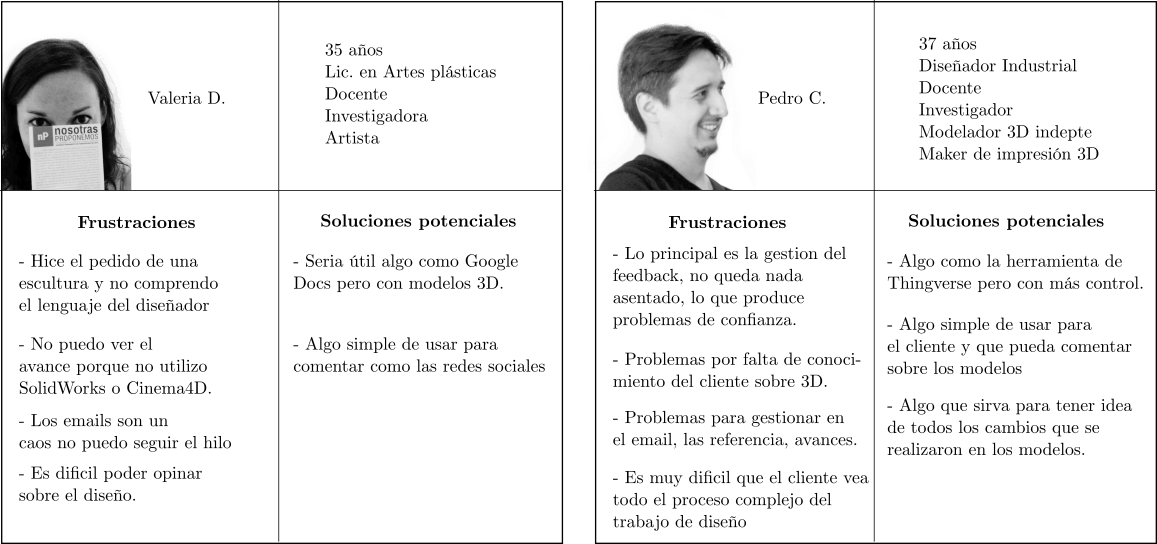
\includegraphics[width=16cm]{Img/Desarrollo/persona1.png}
\centering
\caption{\footnotesize{Personas utilizadas en CoCADa. El usuario sin conocimientos de CAD (Persona A)(izquierda). Usuario profesional (Persona B)(derecha). En la parte superior se especifica la información general del usuario. El cuadrante inferior izquierdo debe contiene las necesidades y  frustraciones respecto la solución actual, los puntos de conflicto específicos que el producto intenta resolver y/o la oportunidad que se trata de capturar con él. El cuadrante inferior derecho contiene las soluciones potenciales, sugeridas por el usuario.}}
\label{fig:persona1}
\end{figure}

\clearpage
\subsection{Funciones o funcionalidades}
\label{section:subhipo}
Con todo el material obtenido se organizan a continuación las sub-hipótesis que deben probarse. 

\begin{longtable}{|p{1cm}|p{4cm}|p{4cm}|p{4cm}| }

\hline
    Núm. & Se desarrolla (función) & Para (persona)  & Para (solución)\\
\hline
1 & Un visor de modelos 3D en la web & Para (Persona A) y  (Persona B) & Solucionar de forma eficiente la visualización de los productos \\

\hline
2 & Un sistema de comentarios asociado a los modelos 3D & Para (Persona A) y (Persona B)  & Discutir sobre los avances del proyecto.
\\

\hline
3 & Un mecanismo para anotaciones sobre los modelos 3D & Para (Persona A)  y (Persona B) & 
Poder comunicar aspectos de diseño entre personas de diferentes disciplinas  \\

\hline
4 & Un sistema para dar de Alta proyectos & Para (Persona B) & Gestionar nuevos proyectos de diseño.
\\

\hline
5 & Un mecanismo para escribir código de modelado & Para (Persona B) & Incorporar diseños y modificarlos mediante scripting \\
\hline
6 & Un mecanismo para ver los cambios o ``versiones" de los diseños & Para (Persona A) y (Persona B) & Visualizar la evolución de los modelos y su estado en una fecha determinada  \\
\hline

7 & Componentes visuales para modificar los parámetros del modelo 3D & Para (Persona A) y (Persona B) & Modificar geometrías de forma intuitiva, sin necesidad de tener conocimientos de programación o de modelado avanzado  \\

\hline
8 & Un mecanismo para inicio de sesión con usuario y contraseña & Para (Persona A) y (Persona B) & El ingreso privado  \\
\hline

\end{longtable}

\begin{center}
 \caption{\footnotesize{Tabla de sub-hipótesis para CoCADa}}
\end{center}

\clearpage
\section{Diseño Colaborativo}
\label{dis-des-colabo}
 
\begin{figure}[ht]
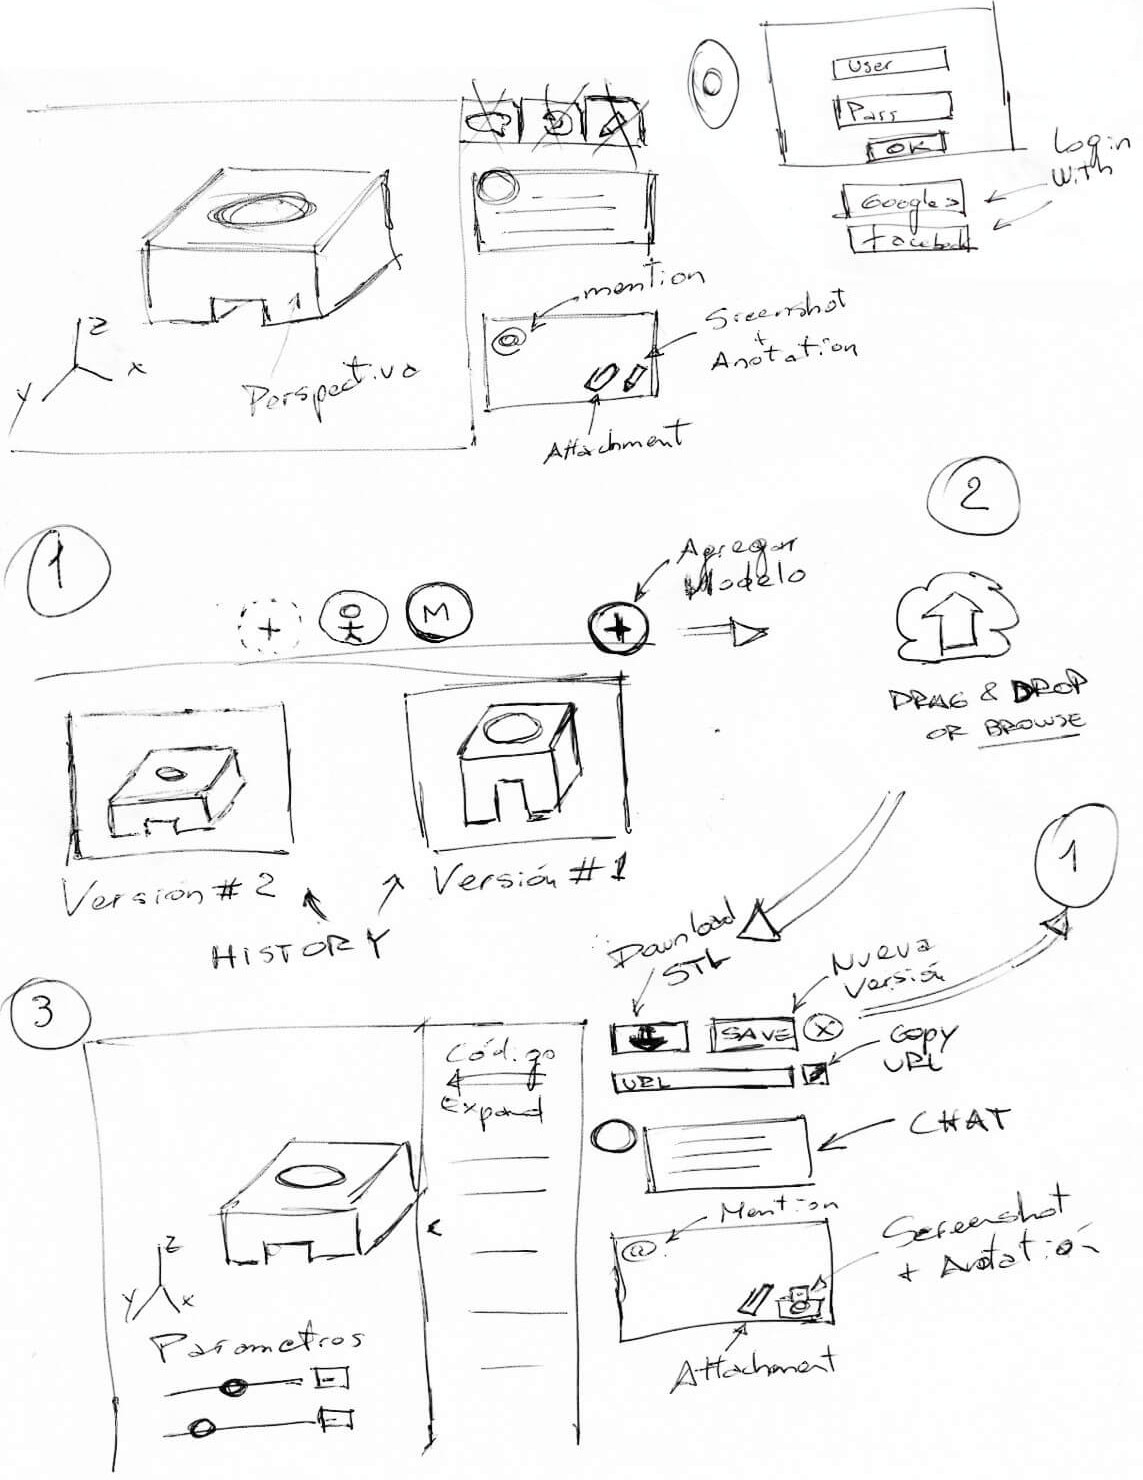
\includegraphics[width=7cm]{Img/UX/edc.jpg}
\centering
\caption{\footnotesize{Resultado del estudio de diseño explicado en la sección \ref{dis-colabo}. Sketchs o bocetos de interfaces de usuario para CoCADa.}}
\label{salida}
\end{figure}

\begin{figure}[ht]
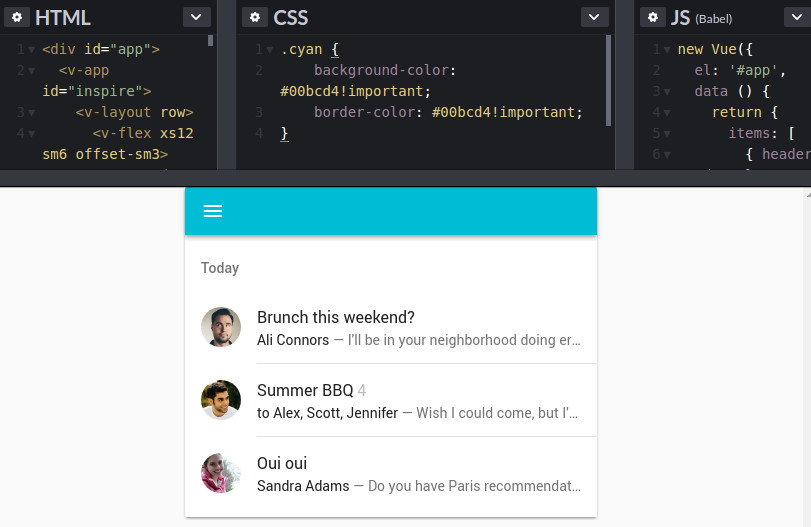
\includegraphics[width=8cm]{Img/Desarrollo/vuety.jpg}
\centering
\caption{\footnotesize{Guía de estilo utilizada en CoCADa. Ejemplo de componente web para conversaciones y su forma de uso mediante código HTML, CSS y javascript.}}
\label{vuetify}
\end{figure}


\clearpage
\section{PMV y experimentos}
\label{pmv-cocada}

El primer PMV o \textbf{Demo \#1} evaluó la \textbf{sub-hipótesis 1} de la tabla de sub-hipótesis: ``\textbf{Un visor de modelos 3D en la web para el usuario (Persona A) y (Persona B) para solucionar de forma eficiente la visualización de los productos}''.\vskip
Se utilizaron tres preguntas para orientar el experimento: 
\begin{enumerate}
    \item \textbf{¿Quién interactuará efectivamente con el prototipo?} \\
    El usuario sin conocimientos de CAD (Persona A).
    \item \textbf{¿Qué se espera aprender de él?} \\
    Aspectos de funcionalidad y usabilidad de la interfaz UI al  momento de interactuar con un modelo 3D.
    \item \textbf{¿Cuánto tiempo se tiene para desarrollar el prototipo?}\\ Aproximadamente 4 días.
\end{enumerate}

Se utilizaron \textbf{prototipos de alta fidelidad} \citep{Gamble2016} %\textquote{\textit{La fidelidad se refiere al nivel de realismo en un prototipo}} . 
para lograr un aspecto y comportamiento similar al de la interfaz definitiva.

En el primer experimento se presentó un prototipo de visor con un modelo 3D (ver figura \ref{fig:feedback0})  %y funcionalidades de zoom (alejar, acercar), rotación y traslación. También se presentan los parámetros para modificar la geometría y el color 
, programado en base 
al código de OpenJSCAD en un tiempo aproximado de 36 horas.

\begin{figure}[ht]
    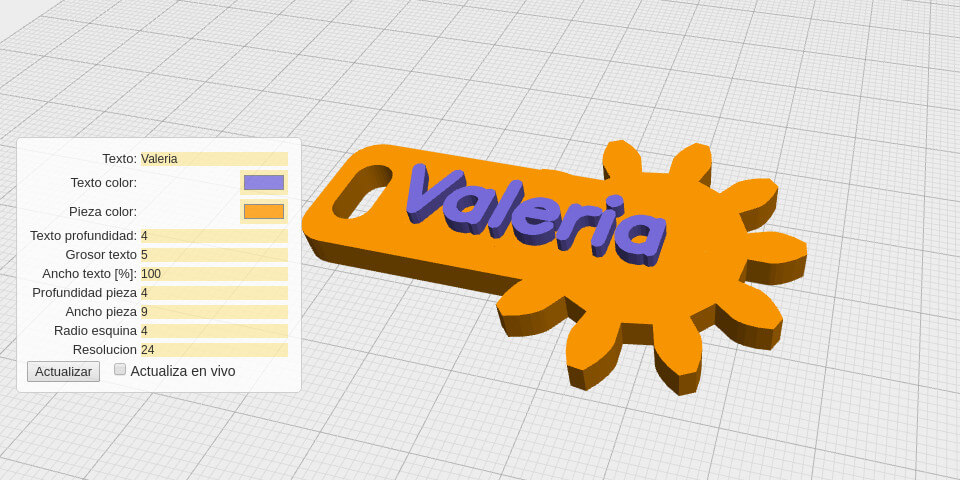
\includegraphics[width=14cm]{Img/Desarrollo/feedback0.jpg}
    \centering
    \caption{\footnotesize{Pantalla  de Demo \#1. Visor con un modelo 3D (centro) y funcionalidades de zoom (alejar, acercar), rotación y traslación. Parámetros para modificar la geometría y el color (izquierda).}}
     \label{fig:feedback0}
\end{figure}


\subsubsection{Características del experimento:} 
Se utilizó una computadora con conexión a internet y un navegador web mostrando el modelo por defecto en la pantalla. El usuario no recibió instrucciones sobre el uso y no tiene limitaciones de tiempo. El evaluador se limitó a observar y registrar la actividad.

\section{Feedback}
\label{feedback}

Al final de la sesión de prueba se realizaron una serie de preguntas sobre la experiencia de usuario, divididas en tópicos. \\ 
Las respuestas posibles fueron: \textbf{Buena, Regular o Mala}. En caso de responder Regular o Mala se realizaron otras 2 preguntas: \textbf{¿Cuál es el inconveniente?} y \textbf{¿Qué sugiere para resolver ese inconveniente?}\\ 
En la siguiente tabla se detallan los tópicos y sus respuestas:

\begin{longtable}{ |p{0.8cm}|p{2.3cm}|p{2.2cm}|p{3.6cm}|p{3.6cm}| }
\hline
     Ítem & Tópico & Experiencia  & Inconveniente & Cómo mejorar\\
\hline
1 & Visualización del Modelo & Buena & - & -\\
\hline
2 & Zoom & Regular & Al hacer demasiado zoom sobre el modelo ocurre que no hay un limite, lo que produce que se rompa la geometría. & Limitar el zoom o ver la posibilidad de volver la visualización a su estado original.
\\
\hline
2 & Rotación & Buena & - & -\\
\hline
3 & Translación & Mala & Al mover demasiado el modelo, ocurre que se pierde la visualización y parece que la escena esta vacía. & Limitar la opción de mover o ver la posibilidad de volver la visualización a su estado original.
\\
\hline
4 & Modificación de parámetros & Regular & Es incómodo ingresar números utilizando el teclado & Agregar un elemento parecido a los que tienen las apps.\\
\hline
\end{longtable}
\begin{center}
    \caption{\footnotesize{Resultados del feedback para Demo \#1}}
\end{center}

\subsection{Resultados y propuestas}
Luego de replicar y analizar las \textbf{experiencias de usuario negativas},  se construyó un prototipo \textbf{Demo \#2} en base al feedback y las recomendaciones del usuario en el experimento con Demo \#1.

\begin{itemize}

    \item \textbf{Zoom} (alejar, acercar). En la figura \ref{fig:feedback1} se puede apreciar como se ``rompe" la geometría. 
    %No se dispone de un mecanismo para la corrección.\vskip 
    \textbf{Solución}: Se agrega un botón de ``Resetear Vista'' (izquierda) para establecer la cámara en la posición original, con el objeto centrado en la pantalla (ver figura \ref{fig:feedback4} , izquierda).
    
    \begin{figure}[h]
    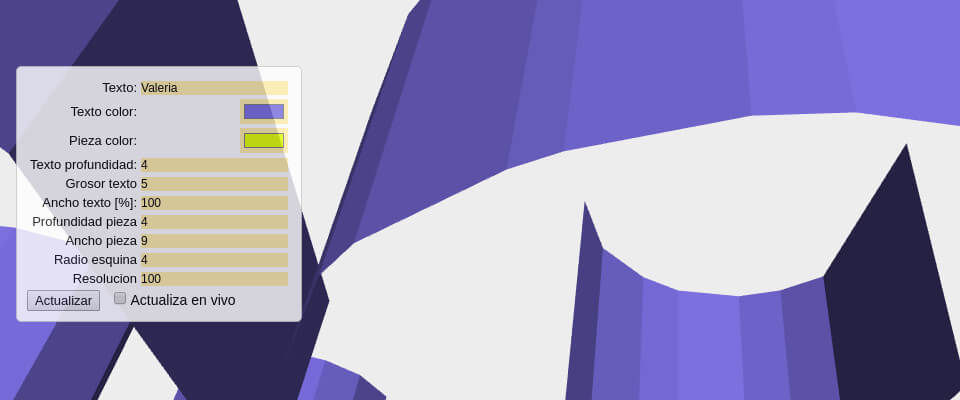
\includegraphics[width=14cm]{Img/Desarrollo/feedback2.jpg}
    \centering
    \caption{\footnotesize{Inconvenientes  con el zoom en Demo \#1. Se ``rompe'' la geometría.}}
     \label{fig:feedback1}
    \end{figure}
    
    \item \textbf{Traslación} (Mover). En la Figura \ref{fig:feedback2} el modelo prácticamente desaparece de la pantalla. %No existe un mecanismo para salir de esta situación. \vskip
    \textbf{Solución}: Se utiliza la misma funcionalidad de el punto anterior.
    
    \item \textbf{Modificación de parámetros}. La mayoría de las personas están acostumbrados a las interfaces con componente gráficos como deslizadores en los que no es necesario escribir  valores numéricos. Tanto en la figura \ref{fig:feedback1} como en la figura \ref{fig:feedback2}(izquierda) no se visualizan este tipo de elementos.\vskip 
    
    \textbf{Solución}: Se agrega un componente \textit{slider} como parámetro ``Texto profundidad" (ver figura \ref{fig:feedback4} , izquierda) para evitar la carga de valores numéricos por teclado. El resto de los campos de texto no se han modificado, intencionalmente, para que el usuario pueda evaluar las diferencias en el uso.

\end{itemize}


   \begin{figure}[h]
    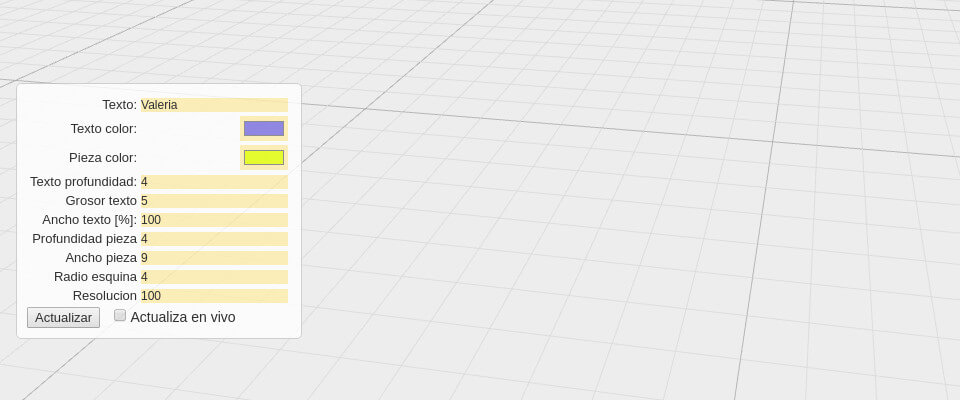
\includegraphics[width=14cm]{Img/Desarrollo/feedback3.jpg}
    \centering
    \caption{\footnotesize{Inconvenientes con la traslación en Demo \#1. El objeto se sitúa fuera del campo de visión. También se observan problemas con la modificación de parámetros (izquierda), el uso de campos de textos no es adecuado para valores numéricos.}}
     \label{fig:feedback2}
    \end{figure}


\begin{figure}[ht]
    \includegraphics[width=14cm]{Img/Desarrollo/feedback4.jpg}
    \centering
    \caption{\footnotesize{Demo \#2. Corrección de inconvenientes hallados en Demo \#1. Se agrega un botón ``Resetear vista'' para solucionar el problema del zoom. Se agrega el componente ``slider'' como parámetro ``Texto profundidad'' para mejorar la experiencia de usuario al modificar los valores numéricos. }}
    \label{fig:feedback4}
\end{figure}

Al finalizar cada experimento se vuelve al ciclo \textit{construir-medir-aprender} visto en la sección \ref{section:pmv}, hasta obtener un prototipo que satisfaga al usuario. De esa manera se obtuvieron recomendaciones interesantes para ser implementadas en el futuro: en el experimento con Demo \#2, el usuario sugirió utilizar la funcionalidad de \textit{reset}\footnote{Reiniciar, en inglés \textit{reset} se conoce como la puesta en condiciones iniciales de un sistema.} pero en los parámetros y de forma individual, un requerimiento de la vista general adaptado a los componentes.\\
Con la tabla de sub-hipótesis y lo aprendido con el usuario en los experimentos, finalmente se estableció la arquitectura de software necesaria para dar soporte a todas las funcionalidades de CoCADa.

\clearpage
\section{Sistema CoCADa}
\label{sistema-cocada}

En la sección \ref{section:subhipo} se identificaron las  funcionalidades que la aplicación debe proveer a los usuarios. Adicionalmente, para una colaboración distribuida, se requiere de la \textbf{Gestión de datos de productos basado en la web} (WPDM), explicada en la sección \ref{sec:pdm}. CoCADa se divide en dos áreas fundamentales: \textit{Back-End} y \textit{Front-End} \citep{mardan2015full}.



    
\subsection{Back-End}
La aplicación de \textit{Back-End} o capa de servicios cuenta con tecnologías para tareas que no pueden ser resueltas directamente por los usuarios como la persistencia de datos y el almacenamiento de archivos. Las tecnologías utilizadas son:

\begin{itemize}

    \item \textbf{Node.js}\footnote{\url{https://nodejs.org/es/}} como web server y entorno de ejecución para JavaScript en el lado del servidor, de la misma manera que lo hacen otros lenguajes como PHP\footnote{\url{http://php.net/manual/es/intro-whatis.php}} o Python. 
    
    \item \textbf{Nuxt.js}\footnote{\url{https://nuxtjs.org/}}. Es un framework para crear aplicaciones isomórficas o universales con Vue.js\footnote{\url{https://vuejs.org/}}. Una aplicación  universal  es  aquella  que su código puede ser ejecutado tanto en el cliente (navegador web) como en el servidor. Nuxt.js incorpora el concepto \textit{Server Side Rendering}  (SSR)\footnote{\url{https://ssr.vuejs.org/#what-is-server-side-rendering-ssr}}.
    El SSR en CoCADa brinda la posibilidad de convertir los  componentes web en cadenas de HTML en el servidor, luego son enviadas al navegador web y se genera la aplicación en el lado del cliente. 
    
    \item \textbf{LoopBack}\footnote{\url{https://loopback.io}}. Es un conjunto de módulos de Node.js que permiten la implementación de APIs \citep{masse2011rest} altamente flexibles. Está basado en el framework \textbf{Express.js}\footnote{\url{https://expressjs.com/es/}} y proporciona funcionalidades para:
    
    - Crear APIs REST dinámicas end-to-end\footnote{End-to-end es un enfoque que involucra la visión global del encadenamiento de procesos y/o actividades, desde que surge una necesidad a satisfacer, hasta que esta es satisfecha} con poca codificación.\\
    - Acceso a datos para los principales motores de bases de datos, servicios SOAP y otras APIs. \\
    - Almacenamiento de archivos o \textit{file storage}.\\
    - Inicio de sesión mediante protocolos de autorización OAuth\footnote{\url{https://oauth.net/2/}}.\\
    Nuxt.js se comunica con LoopBack a través de su API REST , obteniendo como respuesta es un documento JSON.
    
    \item \textbf{MongoDB}\footnote{\url{https://www.mongodb.com/es}}. El enfoque de CoCADa es agnóstico\footnote{Se refiere a la capacidad de interoperabilidad y compatibilidad de un componente de cómputo entre diversos sistemas y ambientes, sin requerir una adaptación especial. } respecto al motor de base de datos, sin embargo, se utiliza MongoDB (NoSQL) para la persistencia de datos. A diferencia de las bases de datos relacionales, los datos se almacenan en tablas, sino mediante documentos en formato JSON. Esto permite que la integración entre MongoDB y javascript sea mucho más directa.

\vskip
\end{itemize}

\begin{figure}[h]
    \includegraphics[width=8cm]{Img/Desarrollo/backendf.png}
    \centering
    \caption{\footnotesize{Backend de CoCADa. Node.js se utiliza como web server y entorno de ejecución para JavaScript. Nuxt.js provee el Server Side Rendering (SSR). Loopback implementa la API REST y gestiona los archivos (File Storage). MongoDB es el motor de bases de datos. Nuxt.js se comunica con LoopBack a través de su API, obteniendo como respuesta un documento JSON.}}
     \label{fig:sistema0}
\end{figure}

\subsubsection{CoCADa API REST}
En esta sección se desarrolla el modelo lógico del sistema, incluyendo el soporte para \textbf{Intercambio de datos Basado en Características} (FBDE) explicado en la sección \ref{FBDE}. El diagrama de la figura \ref{fig:schema} ilustra el esquema de datos y las relaciones entre las entidades. Las especificaciones del modelo y la fuentes de datos (base de datos) se realizan con LoopBack mediante archivos JSON.



\begin{figure}[h]
    \includegraphics[width=10cm]{Img/Desarrollo/cocada-de0.png}
    \centering
    \caption{Modelo de datos para CoCADa. Un Proyecto puede contener versiones de un producto (árbol de historias). Una Versión puede ser utilizada por uno o más usuarios en el marco de trabajo, también soporta conversaciones de estos usuarios a través de Comentarios. Un Usuario puede asumir un rol específico. Un Comentario puede contener uno o más archivos. }
    \label{fig:schema}
\end{figure}

\begin{itemize}
    \item \textbf{Proyecto}: Es la entidad que gestiona la  evolución de los diseños. Puede contener una o más versiones de un producto, también llamado árbol de historias (ver figura \ref{fig:schema}). 
    
    En la figura \ref{fig:schema2} se puede analizar un  proyecto con su respectivas versiones y la evolución de los diseños.
    \begin{figure}[h]
    \includegraphics[width=16cm]{Img/Desarrollo/cocada-de.png}
    \centering
    \caption{\footnotesize{Un proyecto con su árbol de historia o versiones. Se puede apreciar la evolución del producto ordenada por fecha ascendente. La imagen que identifica el $Proyecto \ 1$ es la misma que la última versión del producto. La $Versión \ 1$ se inicia al momento de generar el proyecto, con un modelo de ejemplo (cubo). La $Versión \ 2$ se genera a partir de la anterior, con los cambios efectuados en el código y así sucesivamente.}}
    \label{fig:schema2}
    \end{figure}
    
    \item \textbf{Versión}: Es la representación de un diseño (producto) individual y su información relacionada. También se puede entender como una iteración en el proceso de diseño. 
    
    
    \item \textbf{Usuario}. La entidad representa a los usuarios del sistema. 
    
    \item \textbf{Comentario}. 
    Es la entidad que gestiona los comentarios asociados a una Versión.
    
    \item \textbf{Rol}. Especifica los permisos de los usuarios dentro del sistema, un mismo rol puede ser asignado a diferentes usuarios.
    
    \item \textbf{Archivo}. Esta entidad contiene la dirección web o URL de un archivo, en CoCADa estos archivos se asocian a los comentarios.
    
\end{itemize}

Para facilitar el desarrollo, LoopBack provee una herramienta (\textit{API Explorer}\footnote{\url{https://loopback.io/doc/en/lb3/Use-API-Explorer.html}}) para explorar las entidades, los metodos HTTP disponibles y los \textit{EndPoints}\footnote{Un Endpoint en la API de CoCADa es una URL única que representa un objeto o una colección de objetos.} de la API. En la figura \ref{fig:explorer} se puede ver un modelo ``Versión'' utilizado como prueba.

\begin{figure}[ht]
    \includegraphics[width=16cm]{Img/Desarrollo/strong.jpg}
    \centering
    \caption{\footnotesize{Herramienta API Explorer de LoopBack. Se muestra el contenido de un modelo ``Versión'', se pueden apreciar los datos del producto.}}
    \label{fig:explorer}
\end{figure}

\clearpage
\subsection{Front-End}
\label{front}
En las aplicaciones web, el \textit{Front-End} o capa de presentación implica el uso de las tecnologías con las que interactúa directamente el usuario. Normalmente estas tecnologías son desarrolladas en los lenguajes HTML, CSS, javacript y otros recursos como imágenes y gráficos vectoriales (ver figura \ref{fig:front}). Al ingresar al sistema, se muestra la interfaz de usuario UI también llamada CoCADa APP.

\begin{figure}[h]
    \includegraphics[width=10cm]{Img/Desarrollo/front.png}
    \centering
    \caption{\footnotesize{Frontend de CoCADa. CoCADa APP está compuesta por OpenJSCAD (Lenguaje de descripción) y Vue.js como sistema reactivo + Vuetify (Material Design). WebGL resuelve la representación interna (matemática) en el navegador web.}}
    \label{fig:front}
\end{figure}

Para la implementación se utilizan las siguientes tecnologías:
\begin{itemize}

     \item \textbf{OpenJSCAD} (javascript) como \textbf{lenguaje de descripción CSG} para trabajar en alto nivel y de forma intuitiva con las primitivas, transformaciones, operaciones booleanas, etc. Además provee mecanismos para la manipulación visual de parámetros y exportación de los modelos en formato STL. Una vez procesadas las sentencias del lenguaje de descripción, se traducen a su  \textbf{representación interna} (matemática) vista en la sección \ref{repGeo} mediante la API \textbf{WebGL} del navegador web (ver figura \ref{fig:front}).
     
    \item \textbf{Vue.js}\footnote{\url{https://vuejs.org/}}. Es un framework progresivo para interfaces de usuario, lo que significa que se pueden incorporar herramientas incrementalmente, a medida que aumenta la complejidad de la aplicación. Un ventaja de usar esta tecnología es su característica de sistema \textbf{reactivo} \citep{mezzalira2018front}, manteniendo una interacción constante con su entorno y permitiendo el cambio de estado interno por medio de eventos. 
    Cuando los datos de la interfaz son modificados por alguna acción del sistema o del usuario, por ejemplo: cada vez que se hace una petición al \textit{Back-End} (ver figura \ref{fig:front-backend}), tiene la capacidad de modificar solamente los componentes necesarios, sin necesidad de actualizar toda la aplicación en el navegador web.
    
    \item \textbf{Vuetify}\footnote{\url{https://vuetifyjs.com/en/}}.  Es un framework progresivo orientado a componentes visuales, se basa en el concepto \textit{Material Design}\footnote{\url{https://material.io/design/}}, con elementos reconocibles por los usuarios en la mayoría de las apps. Se utiliza para lograr una experiencia de usuario satisfactoria, en base al diseño establecido en la sección \ref{dis-des-colabo}.\vskip
    
   

\end{itemize}


Para una mejor comprensión de la UI, se hace una  distinción entre pantallas y componentes.


\subsubsection{Pantalla de Proyectos}
Luego del \textit{login} mediante un usuario y contraseña, se muestra una pantalla con el listado de proyectos (ver figura \ref{fig:cocada1})(izquierda).

\begin{figure}[h]
    \includegraphics[width=16cm]{Img/Desarrollo/cocada0.jpg}
    \centering
    \caption{\footnotesize{Pantalla de proyectos (izquierda), en primera instancia se muestra un listado de proyectos con la posibilidad de ver, editar y eliminar los mismos. Al hacer click en la llamada a la acción (botón) en la parte superior derecha de la ventana se agrega un nuevo proyecto. A la derecha se puede observar el formulario de alta para un nuevo proyecto. Los usuarios Persona A y Persona B pueden agregar proyectos.}}
     \label{fig:cocada1}
\end{figure}

\subsubsection{Pantalla de Producto}
Un producto se refiere a una versión especifica del mismo dentro del árbol de historia. 
Al agregar un nuevo producto o al ``ver'' un proyecto del listado, se muestra la pantalla de la figura \ref{fig:cocada2}, correspondiente a la vista de producto. 

\begin{figure}[ht]
    \includegraphics[width=16cm]{Img/Desarrollo/cocada-pantalla.png}
    \centering
    \caption{\footnotesize{Pantalla de Producto. Visor 3D (A) (izquierda). Editor de código (B) (centro). Componente para compartir el modelo (C) (derecha y arriba). Componente de comentarios e historial de modelos (D) (derecha y abajo).}}
     \label{fig:cocada2}
\end{figure}

Los componentes web de la pantalla son:
\begin{itemize}
\item \textbf{A. Componente del Visor 3D} (izquierda). \\


\begin{itemize}
\textbf{A1. Modelo 3D}. Se visualiza el modelo mediante OpenJSCAD y WebGL. Funcionalidades:\\
        \item \textbf{- Zoom} (in - out) mediante el scroll con botón del medio del mouse.\\
        \item \textbf{- Rotación} mediante click con botón izquierdo y moviendo el mouse.\\
        \item \textbf{- Traslación} mediante la tecla shift + botón izquierdo presionados y moviendo el mouse.\\
         \item \textbf{- Reiniciar Vista} mediante el botón ubicado abajo y a la derecha en el visor (sitúa la cámara en su posición original).\\
        \item \textbf{- Descargar STL}. Se genera y descarga el modelo sólido en formato STL (preparado para la fabricación digital)(ver figura \ref{fig:impresion3d}).
        
\end{itemize}

\begin{figure}[ht]
    \includegraphics[width=8cm]{Img/Desarrollo/impresion3d.jpg}
    \centering
    \caption{\footnotesize{Ejemplo de fabricación digital con impresora 3D.}}
     \label{fig:impresion3d}
\end{figure}

\begin{itemize}
\textbf{A2. Parámetros}. Se sitúa en la parte inferior izquierda. Tiene los siguientes componentes:\\
        \item \textbf{- Parámetros de control}.
        Estos campos se configuran previamente mediante código en el componente B (la flecha en la figura \ref{fig:cocada2} indica la relación con el código que genera el campo).\\
        \item \textbf{- Modo Automático}. Permite visualizar automáticamente los cambios, ya sea modificando los parámetros o editando el código. En caso de deshabilitar la opción, los cambios son manuales mediante el botón de la izquierda (útil para modelos con gran cantidad de polígonos). \\
        \item \textbf{- Reiniciar parámetros}. Permite volver los campos de los parámetros al valor por defecto especificado en el código.\\
        
\end{itemize}


\end{itemize}


\begin{itemize}
\item \textbf{B. Componente Editor de código}.

\begin{itemize}
Se sitúa en la parte central del layout y es visible únicamente por el usuario Persona B (diseñador, establecido en la sección \ref{personas}).\\
CoCADa permite editar código javascript en la web con capacidad de resaltado de sintaxis mediante el editor \textbf{Ace Editor}\footnote{\url{https://ace.c9.io/}}. \\Si la opción de ``actualizar automáticamente'' se encuentra habilitada, el código se ejecuta de forma automática. De lo contrario es necesario ejecutar el programa mediante las teclas shift + enter.\\ 
Un script OpenJSCAD debe tener al menos una función definida, la funcion \textit{main()}, que retorna un objeto CSG o un vector (array) de dos o más objetos CSG. 
A continuación se analiza un programa que genera un objeto 3D mediante una operación booleana y transformaciones geométricas. En el código se puede apreciar el uso de una función ordinaria de javascript para calcular un radio, transformaciones sobre los cilindros (rotación), una operación booleana (diferencia) entre una esfera y los tres cilindros; y la definición de parámetros para el usuario. El resultado del script se puede ver  en la figura \ref{fig:jopen}.\\

\end{itemize}

\begin{minted}[baselinestretch=1, bgcolor=white, linenos, fontsize=\footnotesize]{js}

function radiusFromDiameter (d) {// Función de javascript
  return d / 2;
}

function rotcy (rot, r, h) {// Función para rotar los cilindros
  return rotate(rot, cylinder({r: r, h: h, center: true}));
}

function esferaHuecos (params) {
  var size = params.size;
  var hole = params.hole;
  var radius = radiusFromDiameter(hole);
  var height = radiusFromDiameter(size * 2.5);
  // Operación booleana: diferencia entre una esfera y 3 cilindros
  return difference(
    sphere({r: radiusFromDiameter(size)}),
    rotcy([0, 0, 0], radius, height),
    rotcy([90, 0, 0], radius, height),
    rotcy([0, 90, 0], radius, height)
  );
}

function main (params) {
  return esferaHuecos(params);
}

function getParameterDefinitions () { // Parámetros
  return [ { name: 'size', caption: 'Tamaño Esfera:', 
  type: 'slider', initial: 30, min: 5, max: 100, step: 1 },
    { name: 'hole', caption: 'Tamaño Huecos:',
    type: 'slider', initial: 10, min: 5, max: 50, step: 1 } ];
}

\end{minted}

\begin{figure}[h]
\includegraphics[width=7cm]{Img/Desarrollo/esfera-cocada.png}
\centering
\caption{\footnotesize{Modelo 3D resultante de la operación booleana (diferencia) entre una esfera y tres cilindros transformados. En la parte inferior se pueden apreciar los parámetros definidos en el código.}}
\label{fig:jopen}
\end{figure}


Todas las funcionalidades de OpenJSCAD y ejemplos de código se puede estudiar en la guía oficial\footnote{\url{https://openjscad.org/dokuwiki/doku.php}}.


\item \textbf{- Nueva Versión}. Genera una nueva versión del espacio de trabajo (Producto) y luego está disponible en el historial de versiones en el componente (D). El código versionado toma como base los parámetros modificados. 



\end{itemize}


\begin{itemize}
\item \textbf{C. Componente Compartir modelo}.
\begin{itemize}
 Se sitúa en la parte superior derecha de la pantalla. Se comparte un enlace web a una pantalla con visor reducido con el modelo. El objetivo es poder mostrar un diseño a usuarios anónimos.
\end{itemize}

\end{itemize}



\begin{itemize}
\item \textbf{D. Componente de Comentarios e Historial de modelos}.

\begin{figure}[ht]
    \includegraphics[width=14cm]{Img/Desarrollo/comentario00.png}
    \centering
    \caption{\footnotesize{CoCADa. Pestaña de Comentarios: formulario para carga de comentarios en un producto (izquierda). Pestaña de Historial: Listado de productos o versiones (derecha).}}
    \label{fig:comment0}
\end{figure}

\begin{itemize}
 Se sitúa en la parte inferior  derecha del layout. Utiliza un mecanismo de pestañas en inglés \textit{tabs} de manera que la selección de una opción oculte la otra, las opciones son ``Comentarios'' e ``Historial''.\\
 


 \textbf{- Componente de comentarios}. 
 Se accede a través de la primer pestaña o icono en forma de comentario. Su objetivo es lograr la comunicación entre los usuarios en forma de conversación o \textit{chat} (ver \ref{fig:comment0} (izquierda)).
 Existen dos maneras de utilizar imágenes en los comentarios:\\
 

\textbf{Como imagen adjunta}. \\
Presionando el icono de la esquina inferior izquierda del componente (ver figura \ref{fig:comment0} (izquierda)) es posible explorar archivos del dispositivo y adjuntar una imagen. 

\textbf{Como anotaciones en el modelo}. 
\begin{figure}[h]
    \includegraphics[width=12cm]{Img/Desarrollo/comentario2.jpg}
    \centering
    \caption{\footnotesize{ Herramienta para anotaciones sobre los modelos. Se utiliza la herramienta presionando el icono con forma de lápiz. Esto realiza una captura de pantalla del modelo y mediante una herramienta de dibujado permite hacer anotaciones sobre la imagen. Las anotaciones son muy útiles para comunicar de manera directa ideas sobre el modelo y lograr la colaboración entre participantes con diferentes competencias. }}
    \label{fig:comment2}
\end{figure}

\\




\vspace{5mm}
\textbf{- Componente de Historial}.\\
Se accede a través de la segunda pestaña o icono en forma de reloj. Permite visualizar todas las versiones o iteraciones de un producto, en orden cronológico. Una vez que se accede al producto o versión deseada, se puede modificar para generar otra versión. Esta funcionalidad es fundamental para soportar el diseño iterativo, explicado en la sección \ref{chap:cap3}. Ver figura \ref{fig:comment0} (derecha).


\end{itemize}



\end{itemize}


\clearpage
\subsection{Interacción entre Usuarios, Front-End y Back-End}

Mediante el gráfico resumido de la  arquitectura (ver figura \ref{fig:front-backend}) se pueden analizar las interacciones de los usuarios y las áreas del sistema:

\begin{figure}[ht]
    \includegraphics[width=12cm]{Img/Desarrollo/front-back.png}
    \centering
    \caption{\footnotesize{ CoCADa interacción entre usuarios, Front-End y Back-End. }}
    \label{fig:front-backend}
\end{figure}


\begin{enumerate}
    \item El usuario ingresa al sistema utilizando el navegador web (\textit{Fron-End}) mediante una URL, por ejemplo:  \url{http://cocada:3000/proyecto/000001}.
    
    \item Nuxt.js resuelve la petición en el servidor (\textit{Back-End}) según la URL ingresada por el usuario, 
    en caso de requerir recursos de la API se comunica con LoopBack. Finalmente, se genera la aplicación (CoCADa APP) con los datos solicitados y se envía al \textit{Front-End}. A partir de este momento Nuxt.js no vuelve a intervenir.  

   \item El usuario a través de CoCADa APP realiza una acción, por ejemplo: \textit{Login}, listar proyectos, ver un proyecto, generar una nueva versión, etc. El \textit{Front-End} genera la petición API correspondiente mediante Vue.js. %Tanto las acciones como las interacciones en la UI son gestionadas por Vue.js.
   
   \item LoopBack recibe la petición API, se encarga de resolver la acción y responder al \textit{Front-End} mediante documentos en formato JSON. 
   Por ejemplo: Durante el \textit{Login}, se verifica el usuario y contraseña, como respuesta se obtienen los datos de aceptación o denegación. Si la petición es la ``lista completa de los proyectos'', se retorna una colección de proyectos almacenados en la base de datos. Vue.js es el encargado de actualizar los cambios en la UI con los nuevos datos.

\end{enumerate}


%\input{Chapters/4-pruebas}
%-----------------------------------------------------
% Chapter 5: Conclusiones
%-----------------------------------------------------
\chapter{Conclusiones}
\label{chap: cap5}

Según lo investigado, la tendencia actual en el desarrollo de productos es la colaboración (co-diseño) entre personas con diferentes competencias y dispersas geográficamente. Por esto, surgió la necesidad de desarrollar una solución distribuida en la que los participantes puedan colaborar independientemente de su profesión.\vskip
Las herramientas CAD analizadas, en algunos casos no soportan la colaboración o son aplicaciones orientados a un perfil específico de profesionales (ingenieros, arquitectos, diseñadores industriales, etc).\vskip
El uso de \textit{Lean UX} como metodología orientada a la experiencia de usuario (UX) permitió una comprensión de las necesidades reales.
La utilización de la misma durante el desarrollo ha sido satisfactoria, debido a que las iteraciones o experimentos con  prototipos de alta fidelidad (PMV) han permitido evaluar las soluciones de forma objetiva y obtener \textit{feedback} de inmediato.
\vskip
Los usuarios con experiencia en CAD (diseñadores) necesitan crear modelos 3D en un entorno que permita automatizar partes del diseño, de manera que se pueda registrar su evolución. 
En el capítulo \ref{chap: cap2} para tener una mejor comprensión de las herramientas necesarias para dicho entorno, se exploraron algunas aplicaciones de diseño paramétrico especificado en algoritmos, incluido OpenJSCAD. Además, deben poder comunicarse de forma eficiente con otros usuarios (no expertos). \vskip
Por otro lado, los usuarios no expertos necesitan de un marco de trabajo para expresar sus ideas y experimentar de forma intuitiva  con  modelos 3D. %; a través de la manipulación directa, comentarios, anotaciones y  obtención de archivos (STL) preparados para la fabricación digital.
En este sentido, en el capítulo \ref{chap:cap3} se analizaron algunas aplicaciones de referencia que %que
%implementan estas funcionalidades. %
permiten explorar modelos 3D, realizar comentarios, anotaciones, exportar archivos, etc. 
\vskip
Para que CoCADa sea un sistema de CAD distribuido se han implementado características de \textbf{WPDM} (gestión de los datos del producto basados en la web), brindando acceso a usuarios dispersos geográficamente, independientemente de las plataformas de software que utilicen. El registro de la evolución de los diseños se ha logrado mediante la incorporación de los conceptos \textbf{diseño paramétrico} (\textit{scripting}) y \textbf{FBDE} (intercambio de datos basado en características). Se implementan en el WPDM como versiones del producto, también llamado ``árbol de historias''. A su vez, en cada versión (marco de trabajo compartido) se permite la colaboración entre los usuarios (\textbf{co-diseño}) mediante las herramientas para manipular los diseños, comentar, adjuntar archivos y realizar anotaciones sobre los modelos.\vskip

El uso de herramientas \textbf{FLOSS} ha sido fundamental para adaptar el código fuente de otras aplicaciones a las necesidades del proyecto.
Las tecnologías (Node.js, Nuxt.js, LoopBack, Vue.js, Vuetify) permiten emplear el mismo lenguaje de programación Javascript en toda %s las partes de 
la aplicación (\textit{Backend} y \textit{Frontend}), evitando la complejidad de mantener código de diferentes lenguajes.\vskip

Finalmente, la interfaz gráfica UI ha sido diseñada para una experiencia de usuario UX satisfactoria, facilitando así el auto-aprendizaje de los usuarios sin necesitad de un entrenamiento previo. En base a los experimentos, se llega a la conclusión que la aplicación puede ser utilizada en ambientes de gran complejidad técnica como el modelado mecánico y también para uso recreativo, por ejemplo en el diseño de piezas simples para impresión 3D.

Como trabajo futuro resulta interesante implementar comentarios y características propias de redes sociales como \textbf{@nombre} para hacer referencia al usuario destinatario del mensaje, notificaciones, mensajes de audio, etc.\vskip

Así también durante las pruebas, los usuarios sugirieron la posibilidad de visualizar los modelos considerando otros factores (texturas, iluminación, transparencias, etc).
Sería posible extender los modelos sólidos a otras representaciones mediante librerías como Three.js\footnote{\url{https://threejs.org/}} y así obtener otros resultados  en la visualización de productos.\vskip

%%%%%%%%%%%%%%%%%%%%%%%%%%%%


%%%%%%%%%%%%%%%%%%%%%%%%%%%%
% Referencias
\cleardoublepage
\phantomsection
\addcontentsline{toc}{section}{Bibliografía}

\begingroup
\raggedright
\bibliography{Referencias/bib.bib}
\endgroup




%%%%%%%%%%%%%%%%%%%%%%%%%%%%


%%%%%%%%%%%%%%%%%%%%%%%%%%%%
% START ANEXOS
%%%%%%%%%%%%%%%%%%%%%%%%%%%%

% %-----------------------------------------------------
% Anexos
%-----------------------------------------------------
\chapter{Anexos}
\label{chap: ane}
\section{Encuestas}


	% Appendix Title

%\input{Appendices/AppendixB} % Appendix Title

%\input{Appendices/AppendixC} % Appendix Title

%%%%%%%%%%%%%%%%%%%%%%%%%%%%


%%%%%%%%%%%%%%%%%%%%%%%%%%%%
% START APPENDICES
% \appendix
%%%%%%%%%%%%%%%%%%%%%%%%%%%%

% 
%-----------------------------------------------------
% Appendix: Code
%-----------------------------------------------------
\chapter*{Apéndice}
\label{app:code}

\begin{verbatim}
10 PRINT "HELLO WORLD"
\end{verbatim}	% Appendix Title

%\input{Appendices/AppendixB} % Appendix Title

%\input{Appendices/AppendixC} % Appendix Title

%%%%%%%%%%%%%%%%%%%%%%%%%%%%


%%%%%%%%%%%%%%%%%%%%%%%%%%%%
% END DOCUMENT
\end{document}
%%%%%%%%%%%%%%%%%%%%%%%%%%%%